\documentclass[reprint, amsmath,amssymb,aps,pre]{revtex4-2}

\usepackage[pdfborder={0 0 0.5 [3 2]}, plainpages=false]{hyperref}%
\usepackage[left=1in,right=1in,top=1in,bottom=1in]{geometry}%

\usepackage{enumerate}
\usepackage{amsfonts}
\usepackage{amsthm}
\usepackage{bbm}
\usepackage[table,xcdraw]{xcolor}
\usepackage{mathtools}
\usepackage{cool}
\usepackage{graphicx,epsfig}

\usepackage{subcaption}
\captionsetup{font={small},skip=0.25\baselineskip}
\captionsetup{justification=raggedright}
\captionsetup[subfigure]{font={small}, skip=1pt, singlelinecheck=false}

\usepackage[capitalize,nameinlink]{cleveref}
% Per SIAM Style Manual, "section" should be lowercase
\crefname{section}{section}{sections}
\crefname{subsection}{subsection}{subsections}
\Crefname{section}{Section}{Sections}
\Crefname{subsection}{Subsection}{Subsections}

% Per SIAM Style Manual, "Figure" should be spelled out in references
\Crefname{figure}{Figure}{Figures}

% Per SIAM Style Manual, don't say equation in front on an equation.
\crefformat{equation}{\textup{#2(#1)#3}}
\crefrangeformat{equation}{\textup{#3(#1)#4--#5(#2)#6}}
\crefmultiformat{equation}{\textup{#2(#1)#3}}{ and \textup{#2(#1)#3}}
{, \textup{#2(#1)#3}}{, and \textup{#2(#1)#3}}
\crefrangemultiformat{equation}{\textup{#3(#1)#4--#5(#2)#6}}%
{ and \textup{#3(#1)#4--#5(#2)#6}}{, \textup{#3(#1)#4--#5(#2)#6}}{, and \textup{#3(#1)#4--#5(#2)#6}}

% But spell it out at the beginning of a sentence.
\Crefformat{equation}{#2Equation~\textup{(#1)}#3}
\Crefrangeformat{equation}{Equations~\textup{#3(#1)#4--#5(#2)#6}}
\Crefmultiformat{equation}{Equations~\textup{#2(#1)#3}}{ and \textup{#2(#1)#3}}
{, \textup{#2(#1)#3}}{, and \textup{#2(#1)#3}}
\Crefrangemultiformat{equation}{Equations~\textup{#3(#1)#4--#5(#2)#6}}%
{ and \textup{#3(#1)#4--#5(#2)#6}}{, \textup{#3(#1)#4--#5(#2)#6}}{, and \textup{#3(#1)#4--#5(#2)#6}}

% Make number non-italic in any environment.
\crefdefaultlabelformat{#2\textup{#1}#3}

\hypersetup{hidelinks}

\def\noi{\noindent}
\def\T{{\mathbb T}}
\def\R{{\mathbb R}}
\def\N{{\mathbb N}}
\def\C{{\mathbb C}}
\def\Z{{\mathbb Z}}
\def\P{{\mathbb P}}
\def\E{{\mathbb E}}
\def\Q{\mathbb{Q}}
\def\ind{{\mathbb I}}

\DeclareMathOperator{\spn}{span}
\DeclareMathOperator{\ran}{range}

\graphicspath{ {images/} }

\newtheorem{lemma}{Lemma}
\newtheorem{theorem}{Theorem}
\newtheorem{corollary}{Corollary}
\newtheorem{definition}{Definition}
\newtheorem{proposition}{Proposition}
\newtheorem{hypothesis}{Hypothesis}
\newtheorem{remark}{Remark}

\begin{document}

\title{Standing and Traveling Waves in a Model of Modulated One-dimensional Waveguide Arrays}
% JCM: We should think about the title

\author{Ross Parker}
\affiliation{Department of Mathematics, Southern Methodist University, 
Dallas, TX 75275, USA}
\email{rhparker@smu.edu}

\author{Jes\'us Cuevas-Maraver}
\affiliation{Grupo de F\'{\i}sica No Lineal, Departamento de F\'{\i}sica Aplicada I,
Universidad de Sevilla. Escuela Polit\'{e}cnica Superior, C/ Virgen de Africa, 7, 41011-Sevilla, Spain}
\affiliation{Instituto de Matem\'{a}ticas de la Universidad de Sevilla (IMUS). Edificio
Celestino Mutis. Avda. Reina Mercedes s/n, 41012-Sevilla, Spain}

\author{P.\,G. Kevrekidis} 
\affiliation{Department of Mathematics and Statistics, University of Massachusetts, Amherst MA 01003, USA}
\email{kevrekid@math.umass.edu}

\author{Alejandro Aceves}
\affiliation{Department of Mathematics, Southern Methodist University, 
Dallas, TX 75275, USA}
\email{aaceves@smu.edu}

\begin{abstract}
In the present work, we study coherent structures in a one-dimensional discrete nonlinear 
Schr{\"o}dinger lattice  in which the coupling between waveguides is periodically modulated. Evolution experiments starting with single-site initial conditions show that the system exhibits two fundamentally different behaviors, depending on the power of the initial condition. Low power initial conditions give rise to solutions which move unidirectionally in the lattice, whereas high power initial conditions yield stationary solutions. We explain these two behaviors, as well as the nature
of the transition between the two regimes, by analyzing a simplification of the model where the couplings between waveguides are given by step functions. We then numerically construct both stationary and moving coherent structures, which are solutions reproducing themselves exactly after an integer multiple of the coupling period. For the stationary solutions, which are true periodic orbits, we use Floquet analysis to determine the parameter regime for which they are spectrally stable. The moving solutions are characterized by small-amplitude, oscillatory tails. We locate a set of parameters for which these tails disappear; these parameters are independent of the lattice size, and numerical evolution experiments suggest that moving solutions with these parameters are stable.
\end{abstract}

%JCM: I have found throughout the paper that |u_n|^2 is dubbed as power instead of density, whereas power is reserved for the summation of the density

\maketitle

\section{Introduction}\label{sec:intro}

The study of lattice nonlinear dynamical
systems with dispersive properties has been
an important component of recent efforts
both within the field of nonlinear 
optics~\cite{LEDERER20081} and within that
of atomic condensates~\cite{RevModPhys.78.179},
among others. In the former realm, the relevant
models considered the propagation of light
in coupled arrays of optical waveguides, while
in the latter setting, they explored the
evolution of the mean-field wavefunction in the
context of deep optical lattices.
In both cases, the prototypical model
of interest (also as an envelope wave
model of other discrete settings, including
mechanical and electrical lattices~\cite{remoissenet,DP06}) has been the
prototypical discrete nonlinear Schr{\"o}dinger (DNLS)
lattice~\cite{kev09}.

Progressively, over the past few years, a
topic that has been gaining significant
traction has been the exploration of
topological features in both linear and
nonlinear systems exhibiting wave dynamics.
Indeed, relevant studies have already been
summarized in a diverse host of fields including,
but not limited to photonics \cite{Ozawa2019},
phononics~\cite{Ma2019,Susstrunk2016}, 
metamaterials~\cite{Bertoldi}, as well
as cold
atom physics~ \cite{Cooper2019}. The resulting
interplay of (especially) nonlinearity
and topology has been leveraged to 
produce solitonic excitations and
domain walls induced by topological
bands~\cite{Lumer2013, Solnyshkov2017, Smirnova2019, Marzuola2019, Mukherjee2020,Chen2014, Hadad2017, Poddubny2018}, to generate states robustly propagating
on domain edges~\cite{Ablowitz2014, Leykam2016, Kartashov2016, Snee2019, Tao2020}, to defy
discreteness-induced barriers such as the famous
Peierls-Nabarro barrier~\cite{Abl21a}, as well as
to achieve unidirectional, uninhibited propagation
around lattice defects in topological lattices~\cite{Abl19a}. These intense recent efforts
have been recently summarized, e.g., in~\cite{Smirnova2020,Ma2021}, and also in the very recent
and detailed review of~\cite{cole}. 

Our focus herein is to combine these two
fundamental ingredients, nonlinearity and
topology in the spirit of a sequence of
highly influential recent experiments 
of Rechtsman and collaborators~\cite{Mukherjee2020,recht21,PhysRevLett.128.113901,Jurgensen2021}. The first one of these works~\cite{Mukherjee2020} has showcased the 
experimental realization of Floquet 
solitons in a topological bandgap, the numerical
existence and stability of which we subsequently
explored in~\cite{PhysRevE.105.044211}. More recently,
such dispersive nonlinear systems
with a coupling dependent on the evolution variable
were proposed as a suitable realization of nonlinear
Thouless pumps~\cite{PhysRevLett.128.113901} and the
topological  properties of the bands such as the Chern
number were argued to govern the resulting soliton motion.
In~\cite{Jurgensen2021}, the analogy with the quantum
Hall effect and the original proposal of the Thouless
pump~\cite{PhysRevB.27.6083} was taken further
by studying how
nonlinearity acts to quantize transport via soliton formation and spontaneous symmetry-breaking bifurcations.

In the present work, we revisit the system analyzed
in~\cite{Jurgensen2021}, but now depart from the 
adiabatic regime of focus therein. 
By doing so, we enable the computation of numerically
exact both {\it stationary}, but importantly also {\it traveling}
solutions. Importantly, not only do we motivate such waveforms
by ``generic'' dynamical evolution experiments, but we also use
a toy variant of the model which involves piecewise-constant
coupling strengths (in a way reminiscent of the celebrated
Kronig-Penney model~\cite{kronig}). There, it becomes evident
that at a qualitative level the transition between standing and
traveling waves mirrors the celebrated self-trapping transition
of DNLS dimer~\cite{Kenkre1986}. The latter may be a quite relevant
insight towards understanding the symmetry breaking transitions
and dynamics within the intensely studied topic of nonlinear Thouless
pumps. 

Our presentation is structured as follows. In section II we present
the theoretical setup and our quantitative diagnostics used in the model
of interest. 
In \cref{sec:rescaling}, we rescale the model so that we can use the propagation distance $L$ as a parameter.
We subsequently turn to numerical computations in section III, starting
with the single-site initial condition evolutions and then obtaining
insights from the simplified piecewise-constant coupling model.
In \cref{sec:singlesite}, we perform evolution experiments starting with a single-site initial condition which demonstrate that there are two fundamental behaviors to the system. For low initial power, the initial intensity moves either to the left or to the right in the lattice. The direction of motion depends on the lattice site chosen for the initial condition. For high initial power, the initial intensity remains confined to a single lattice site. In addition, there does not appear to be a sharp transition between these two behaviors as the starting power is continuously varied.
In \cref{sec:simplified}, we consider a simplification of the model in which the coupling between waveguides is given by step functions. An analysis of this simplified model for an optical dimer explains these two observed behaviors, as well as the lack of a sharp transition between them.
%Armed with this phenomenology and qualitative understanding, we explore
%exact  computations of both standing and traveling solutions, their stability,
%and even the collisions of traveling waveforms. 
In \cref{sec:coherent}, we numerically construct both stationary and traveling coherent structures. As opposed to what occurs with single-site initial conditions, these coherent structure reproduce themselves exactly after an integer multiple of the coupling period. We use Floquet theory to determine the spectral stability of the stationary coherent structures, which are periodic orbits of the system.
Finally, in section IV we
summarize our findings and present our conclusions, including a number
of directions for future study.


%This paper is organized as follows. 
%After briefly looking at collisions between leftward- and rightward-moving %solutions in \cref{sec:collisions}, we summarize our findings and present some
%directions for future study in \cref{sec:conclusions}.



\section{Theoretical Analysis}

\subsection{Mathematical Model}

As discussed above and motivated by experiments such as those of~\cite{PhysRevLett.128.113901,Jurgensen2021}, we study light propagation in an array of coupled optical waveguides, where the coupling is periodically modulated along the axis of light propagation. Mathematically, this is described by the 
non-autonomous variant of the DNLS model of the form:
\begin{equation}\label{eq:DNLSH}
i \frac{d u_n}{d z} + \sum_m H_{n,m}(z)u_m + g|u_n|^2 u_n = 0,
\end{equation}
where $u_n(z)$ is the complex amplitude of the waveguide at site $n$ in the integer lattice, $z$ is the propagation distance (in the direction along the waveguides), and $H$ is the linear, $z$-dependent (i.e., dependent on the
evolution variable) tight-binding Hamiltonian. The parameter $g$ quantifies the strength of the cubic Kerr nonlinearity. For the Hamiltonian $H$, as in \cite{Jurgensen2021}, we use an off-diagonal implementation of the Aubry-Andr\'e-Harper model \cite{Aubry1980,Harper1955} with three sites per unit cell. 
\begin{equation}\label{eq:model}
i \frac{d u_n}{d z} + J_n(z) u_{n+1} + J_{n-1}(z)u_{n-1} + g|u_n|^2 u_n = 0.
\end{equation}
The $z$-dependent coupling functions $J_n(z)$ are periodic in $z$ with spatial period $L$, which we will refer to as the coupling period. We note that \cite{Jurgensen2021} considers this model in the adiabatic regime, i.e. for very large $L$ (see, for example, \cite[Figure 2]{Jurgensen2021}, where $L=8000$), in which case the system is approximately at equilibrium for every $z$. 
This is a point central to the analysis presented therein which is 
explicitly geared towards (and limited to) such an adiabatic regime.
By contrast, the parameter regime we consider herein is that of relatively small $L$, e.g. $L=2\pi$. In this case, stationary solutions are (genuine) periodic orbits of the system, which, in turn, enables us to use the tools of Floquet analysis to determine their spectral stability.
The choice of $J_n(z)$
\begin{equation}\label{eq:Jn}
J_n(z) = J_0 + C \cos^2\left( \frac{\pi}{L}z + \frac{4 \pi}{3} n + \frac{\pi}{6} \right)
\end{equation}
groups the lattice sites into unit cells comprising three waveguides each (\cref{fig:J}, see also \cite[Figure 1]{Jurgensen2021}), since $J_n(z) = J_m(z)$ for $m \equiv n\,(\text{mod}\,3)$. This choice of $J_n(z)$ is (slightly) modified from Equation (3) in the supplement of \cite{Jurgensen2021}; squaring the cosine function ensures that the coupling is always positive.
\begin{figure}
    \centering
    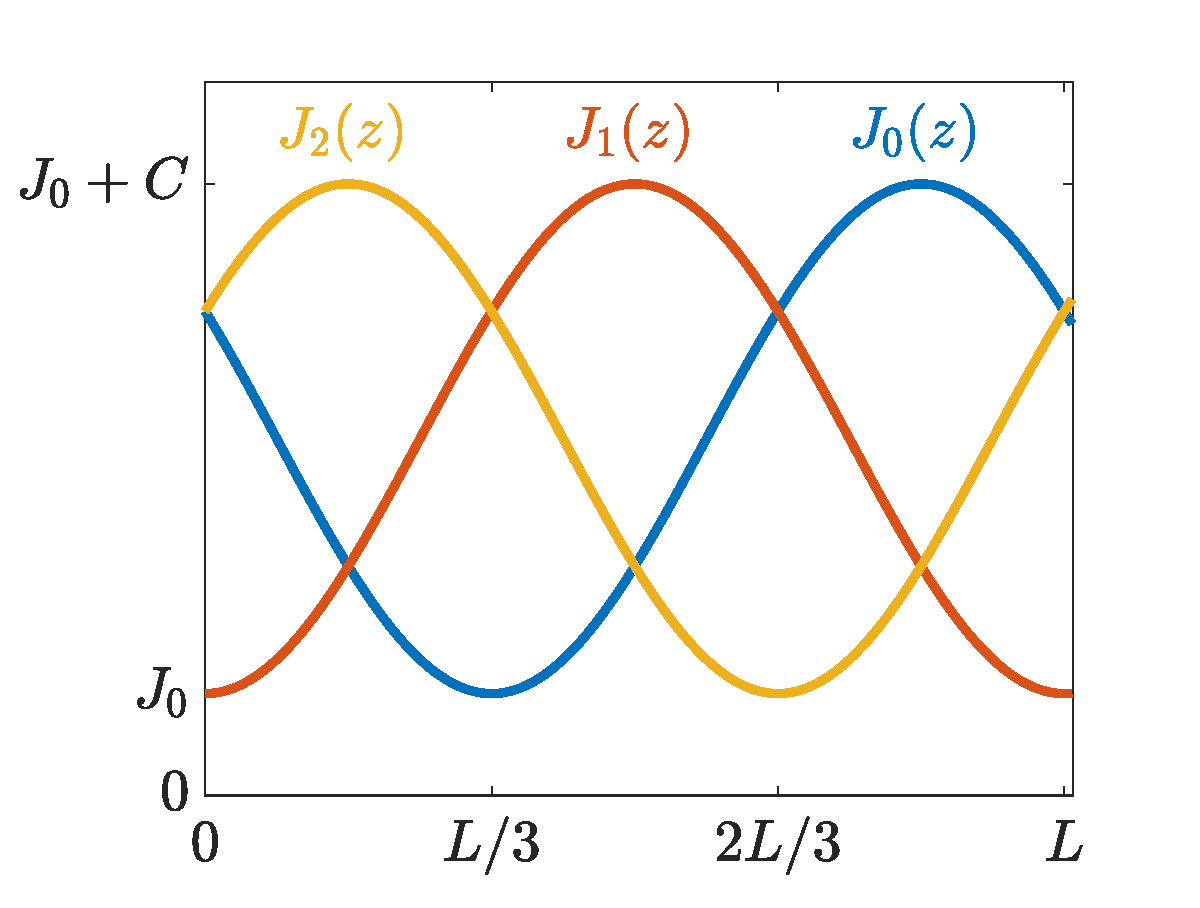
\includegraphics[width=8cm]{J.eps}
    \caption{Coupling functions $J_0(z)$, $J_1(z)$, and $J_2(z)$ of $z$-dependent nearest-neighbor couplings over one spatial period $L$.}
    \label{fig:J}
\end{figure}
When $C = 0$, the nearest neighbor coupling is constant, and Eq.~\cref{eq:model} reduces to the ordinary DNLS with coupling via the discrete second difference operator \cref{eq:modelDNLS}, written in a co-rotating frame with frequency $2 J_0$, which is given by
\begin{equation}\label{eq:modelDNLS}
i \frac{d u_n}{d z} + J_0( u_{n+1} - 2 u_n + u_{n-1}) + g|u_n|^2 u_n 
+ 2 J_0 u_n 
= 0.
\end{equation}
% Comment: as written there were no assumptions or corrotating frame since 
% the terms was added and then subtracted...Please check the commenting out. RP: I subtracted the 2 J_0 u_n to get the second difference operator in the canonical form of DNLS, then had to add it back, which is what puts us in the corotating frame.

\subsection{Model Rescaling and Density Evolution}\label{sec:rescaling}

In order to use the spatial period $L$ as a parameter, we rescale the propagation distance using the change of variables $z = L Z$ so that the coupling period is always 1.
\begin{equation}\label{eq:modelZ}
\begin{aligned}
i \frac{1}{L} \frac{d u_n}{d Z} &+ J_n(Z) u_{n+1} + J_{n-1}(Z)u_{n-1} + g|u_n|^2 u_n = 0 \\
J_n(Z) &= J_0 + C \cos^2\left( \pi Z + \frac{4 \pi}{3} n + \frac{\pi}{6} \right)
\end{aligned}
\end{equation}
At any propagation distance $Z$, the power of the solution is the squared $\ell^2$ norm of the solution
\begin{equation}
P(u_n) = \sum_{n} | u_n(Z) |^2,
\end{equation} 
where the sum is taken over the entire lattice. The power is conserved, i.e., $P(u_n)$ is independent of $Z$. Using equation \cref{eq:modelZ} and its complex conjugate, we derive the flux equations
% Comment: maybe give some reference of where it is referred to like that?
% Alternatively, just more "modestly" refer to this as the flux equations? 
% RP: I just used "flux equations" for simplicity.
for the density matrix elements $\rho_{mn} = \overline{u_n} u_m$
\begin{equation}\label{eq:rhoeq}
\begin{aligned}
\frac{d \rho_{mn}}{dZ} &= iL \Big[ J_m(Z) \rho_{m+1,n} + J_{m-1}(Z) \rho_{m-1,n} \\
&\qquad -J_n(Z) \rho_{m,n+1} - J_{n-1}(Z) \rho_{m,n-1} \big] \\
&\qquad + iLg\left( \rho_{mm} - \rho_{nn} \right) \rho_{mn}
\end{aligned}
\end{equation}
The evolution of the density (or optical intensity) of the solution at lattice site $n$, which is given by $\rho_{nn} = | u_n |^2$, is
\begin{equation}\label{eq:powerevol}
\begin{aligned}
\frac{d\rho_{nn} }{dZ} &= iL \Big[ J_n(Z) \rho_{n+1,n} + J_{n-1}(Z) \rho_{n-1,n} \\
&\qquad -J_n(Z) \rho_{n,n+1} - J_{n-1}(Z) \rho_{n,n-1} \big] \\
&= -2L\,\text{Im}\Big[ J_n(Z) \rho_{n+1,n} + J_{n-1}(Z) \rho_{n-1,n} \Big],
\end{aligned}
\end{equation}
where we used the fact that $\rho_{n,m} = \overline{\rho_{m,n}}$.
Using the last line of \cref{eq:powerevol}, we define the leftward and rightward fluxes at each lattice site $n$ by
\begin{equation}
\begin{aligned}
Q_n^L(Z) &= -2L\,J_{n-1}(Z)\,\text{Im}\,\rho_{n-1,n} \\
Q_n^R(Z) &= -2L\,J_{n-1}(Z)\,\text{Im}\,\rho_{n+1,n} 
\end{aligned}
\end{equation}
where positive flux denotes flow of power into site $n$. These obey the relations $Q_n^R(Z) = -Q_{n+1}^L(Z)$ and $Q_n^L(Z) = -Q_{n-1}^R(Z)$ since, for example, density flowing into site $n$ from the right must flow out of site $n+1$ from the left.
%Since the power of the solution is conserved, $Q_n^R(Z) = -Q_{n+1}^L(Z)$ and %$Q_n^L(Z) = -Q_{n-1}^R(Z)$.
% Comment: I am not sure that I agree with this statement
% (except perhaps in special cases). Recall the point that
% Jesus also made, namely that $\rho_{nn}$ is not a priori
% a conserved quantity (the sum of all of them is, %
% telescopically conserved). 

\section{Numerical Computations}

\subsection{Single site evolution}\label{sec:singlesite}

As an initial experiment, we consider evolution dynamical
simulations starting with a single excited site at $Z=0$. Unless otherwise specified, the parameters in the section are $g=1$, $L=2\pi$, $J_0 = 0.05$, and $C=0.4$, and the simulations are run on a finite lattice with $m=30$ lattice points, with periodic boundary conditions on the ends of the lattice (i.e., a
ring allowing for waves to loop around when they reach the 
boundaries). For a single-site initial condition of sufficiently high power (above a threshold between $P=2.25$ and $P=2.5$ for 
% Comment: please check the rewrite!
initial intensity at $n=0$, and between $P=2.15$ and $P=2.25$ for initial intensity at $n=-1$), the power remains concentrated at a single site, and this appears to be stable as $Z$ evolves (see bottom right panel of Figs.~\ref{fig:timestep0} and \ref{fig:timestep-1}). As the initial power is lowered, this single-site solution becomes prone to mobility; in both cases, this leads the initially concentrate intensity to initially leak to the right within the lattice before dispersing throughout the lattice (bottom left panel of Figs.~\ref{fig:timestep0} and \ref{fig:timestep-1}). For lower power (between $P=0.5$ and $P=1$), the initial intensity moves either to the left in the lattice (for excited site at $n=0$, see top of \cref{fig:timestep0}) or to the right (for excited site at $n=-1$, see top of \cref{fig:timestep-1}) before dispersing
through the lattice. One explanation for this observation is as follows. For the first third of the period ($Z \in [0,1/3]$), the strongest coupling is between site $n=0$ and $n=-1$ via $J_{-1} = J_2$ (see \cref{eq:Jn} and \cref{fig:J}), so intensity can flow to the left from $n=0$ to $n=-1$, which occurs when the initial power is sufficiently low. For $Z \in [1/3,2/3]$, the strongest coupling is between $n=-1$ and $n=-2$, and for $Z \in [1/3,2/3]$, the strongest coupling is between $n=-2$ and $n=-3$, thus we expect the intensity to travel three sites to the left over one period. Similarly, for the rightward moving solution starting at $n=-1$, the rightward coupling is strongest for a rightward sequence of sites on the $Z$ intervals $[0,1/3]$, $[2/3,1]$, and $[4/3,5/3]$, thus this solution moves to the right three sites in two periods. A similar rightward moving behavior occurs when the initial excited site is $n=1$ (not shown). The first coupling for $n=1$ is to the right on the interval $[1/3, 2/3]$; the behavior is then similar to that of the rightward moving solution for $n=-1$. We believe that this
intuitive explanation is quite straightforward and, thus,
appealing towards understanding solitary wave motion in such
non-autonomous discrete nonlinear systems.

\begin{figure}
    \centering
    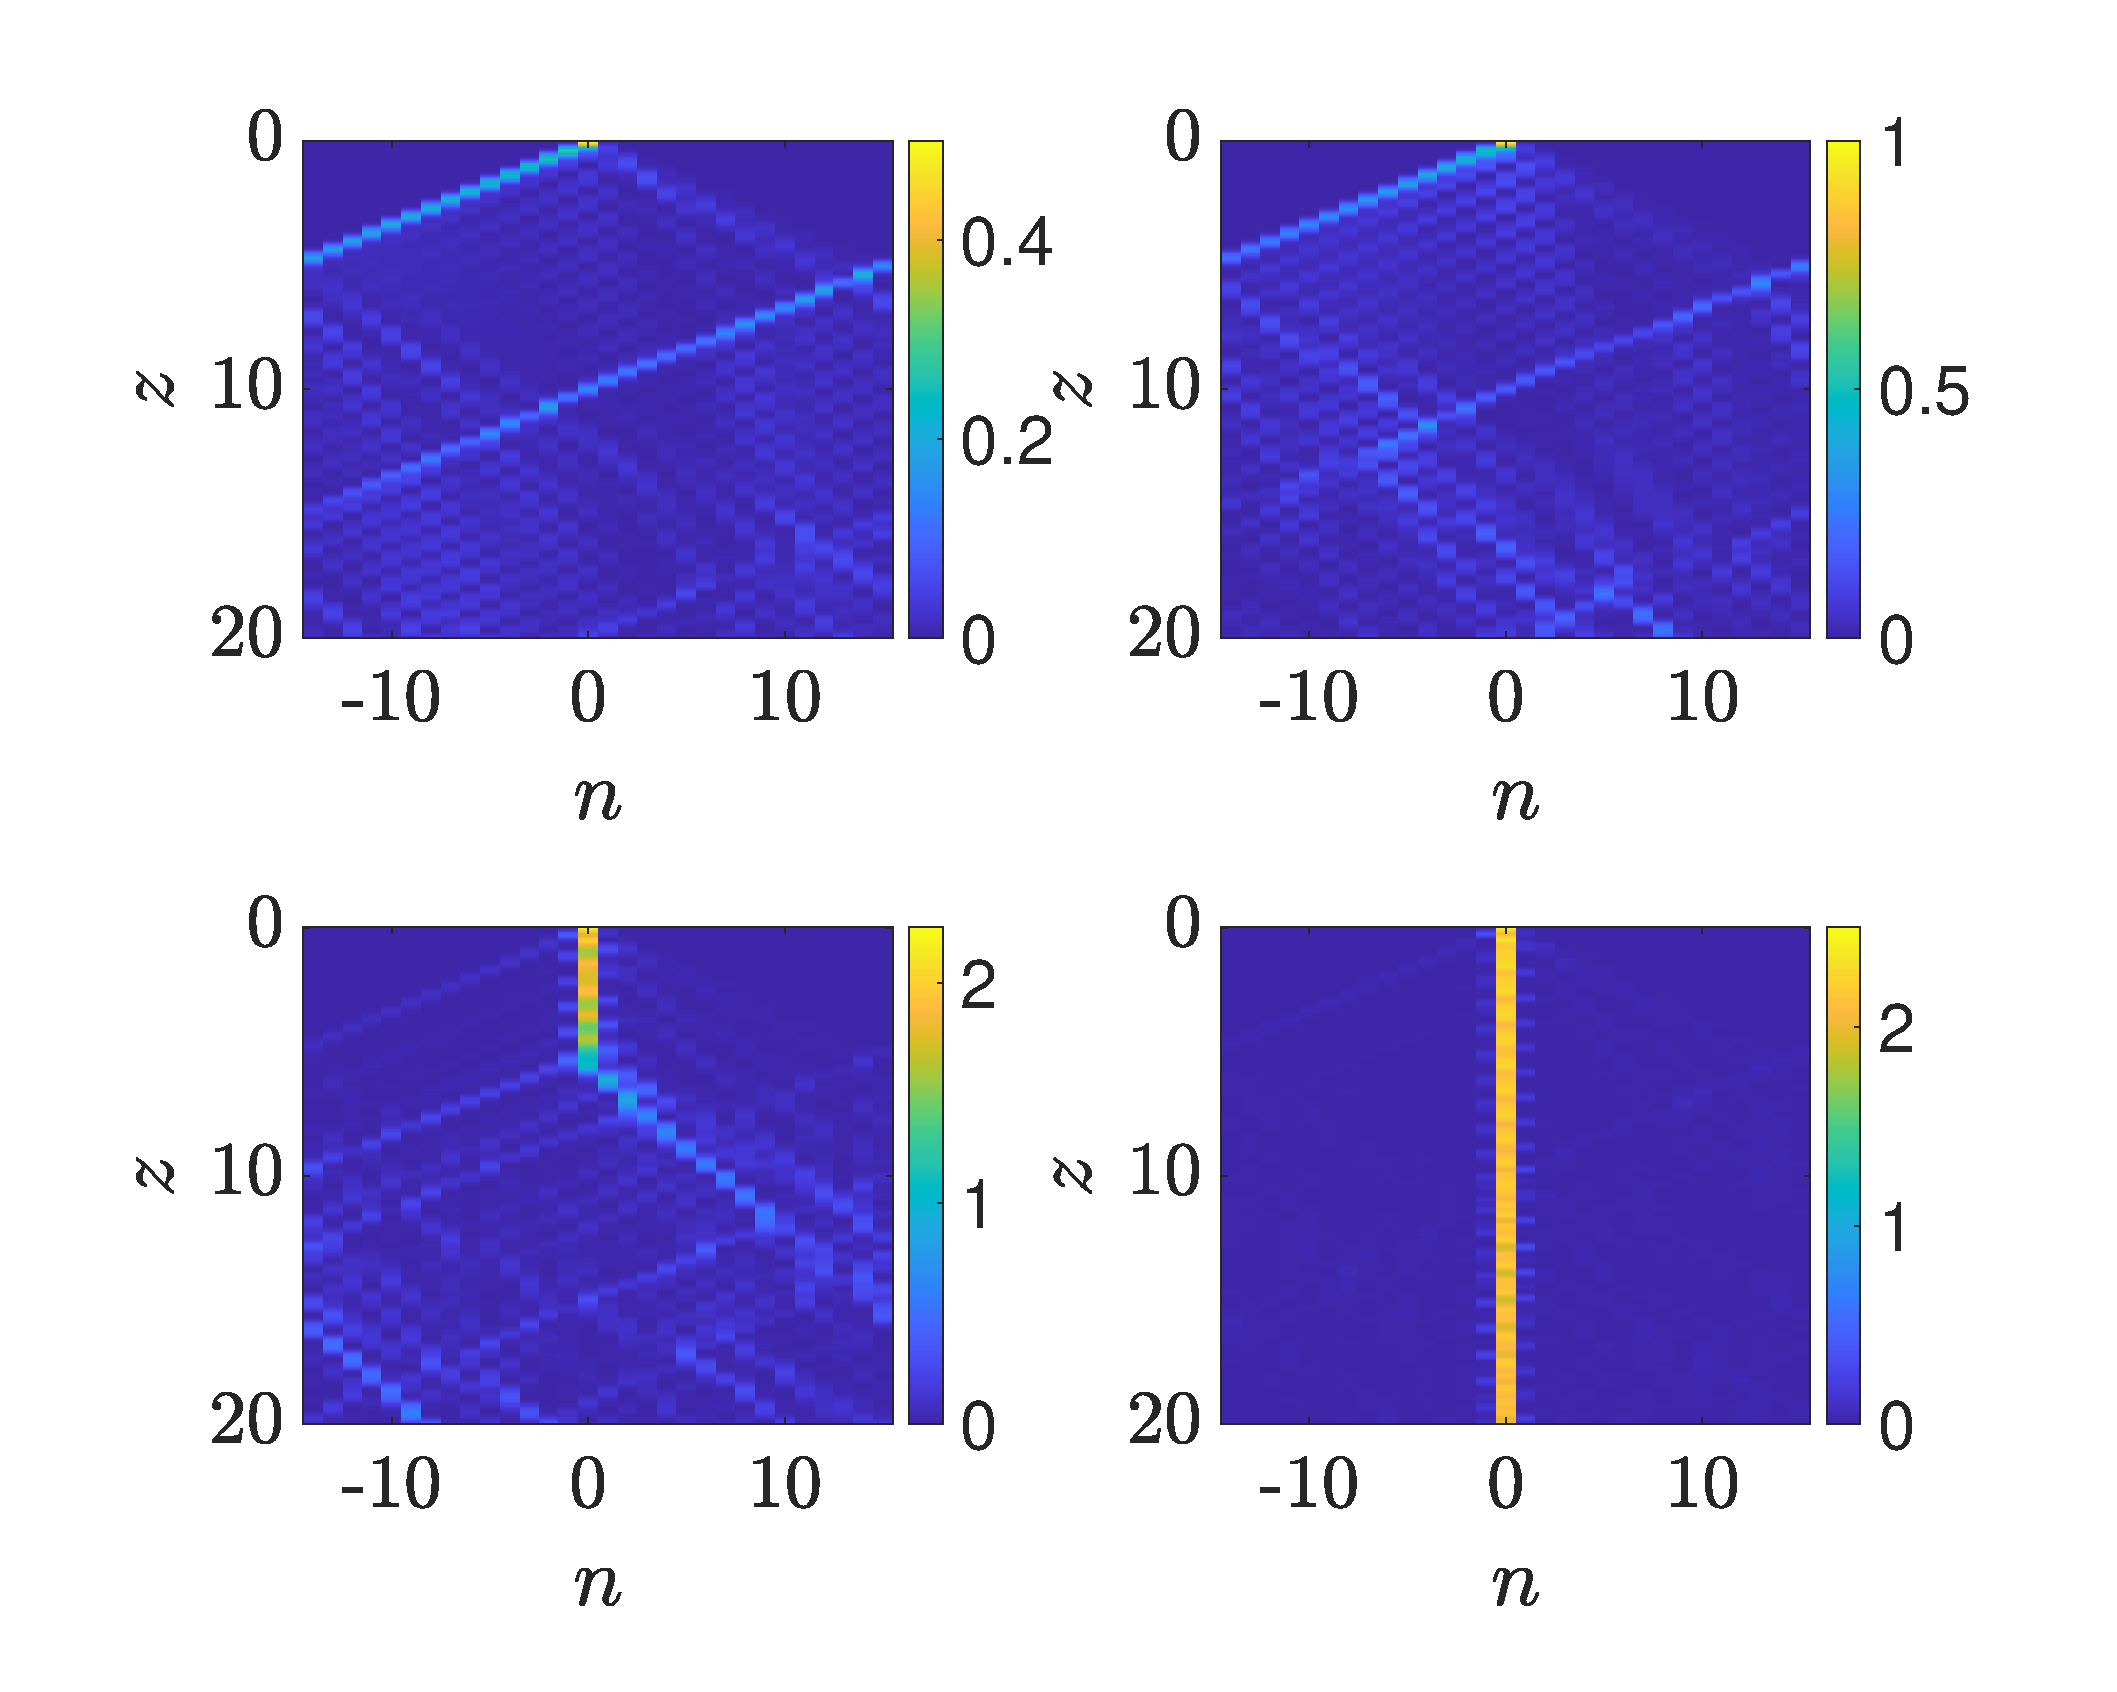
\includegraphics[width=9cm]{timestep0.eps}
    \caption{Colormap showing the density of the solution of equation \cref{eq:modelZ} evolving in $Z$, starting with a single excited site at $n=0$ with power $P=0.5,1,2.25,2.5$ (left to right, top to bottom). }
    \label{fig:timestep0}
\end{figure}

\begin{figure}
    \centering
    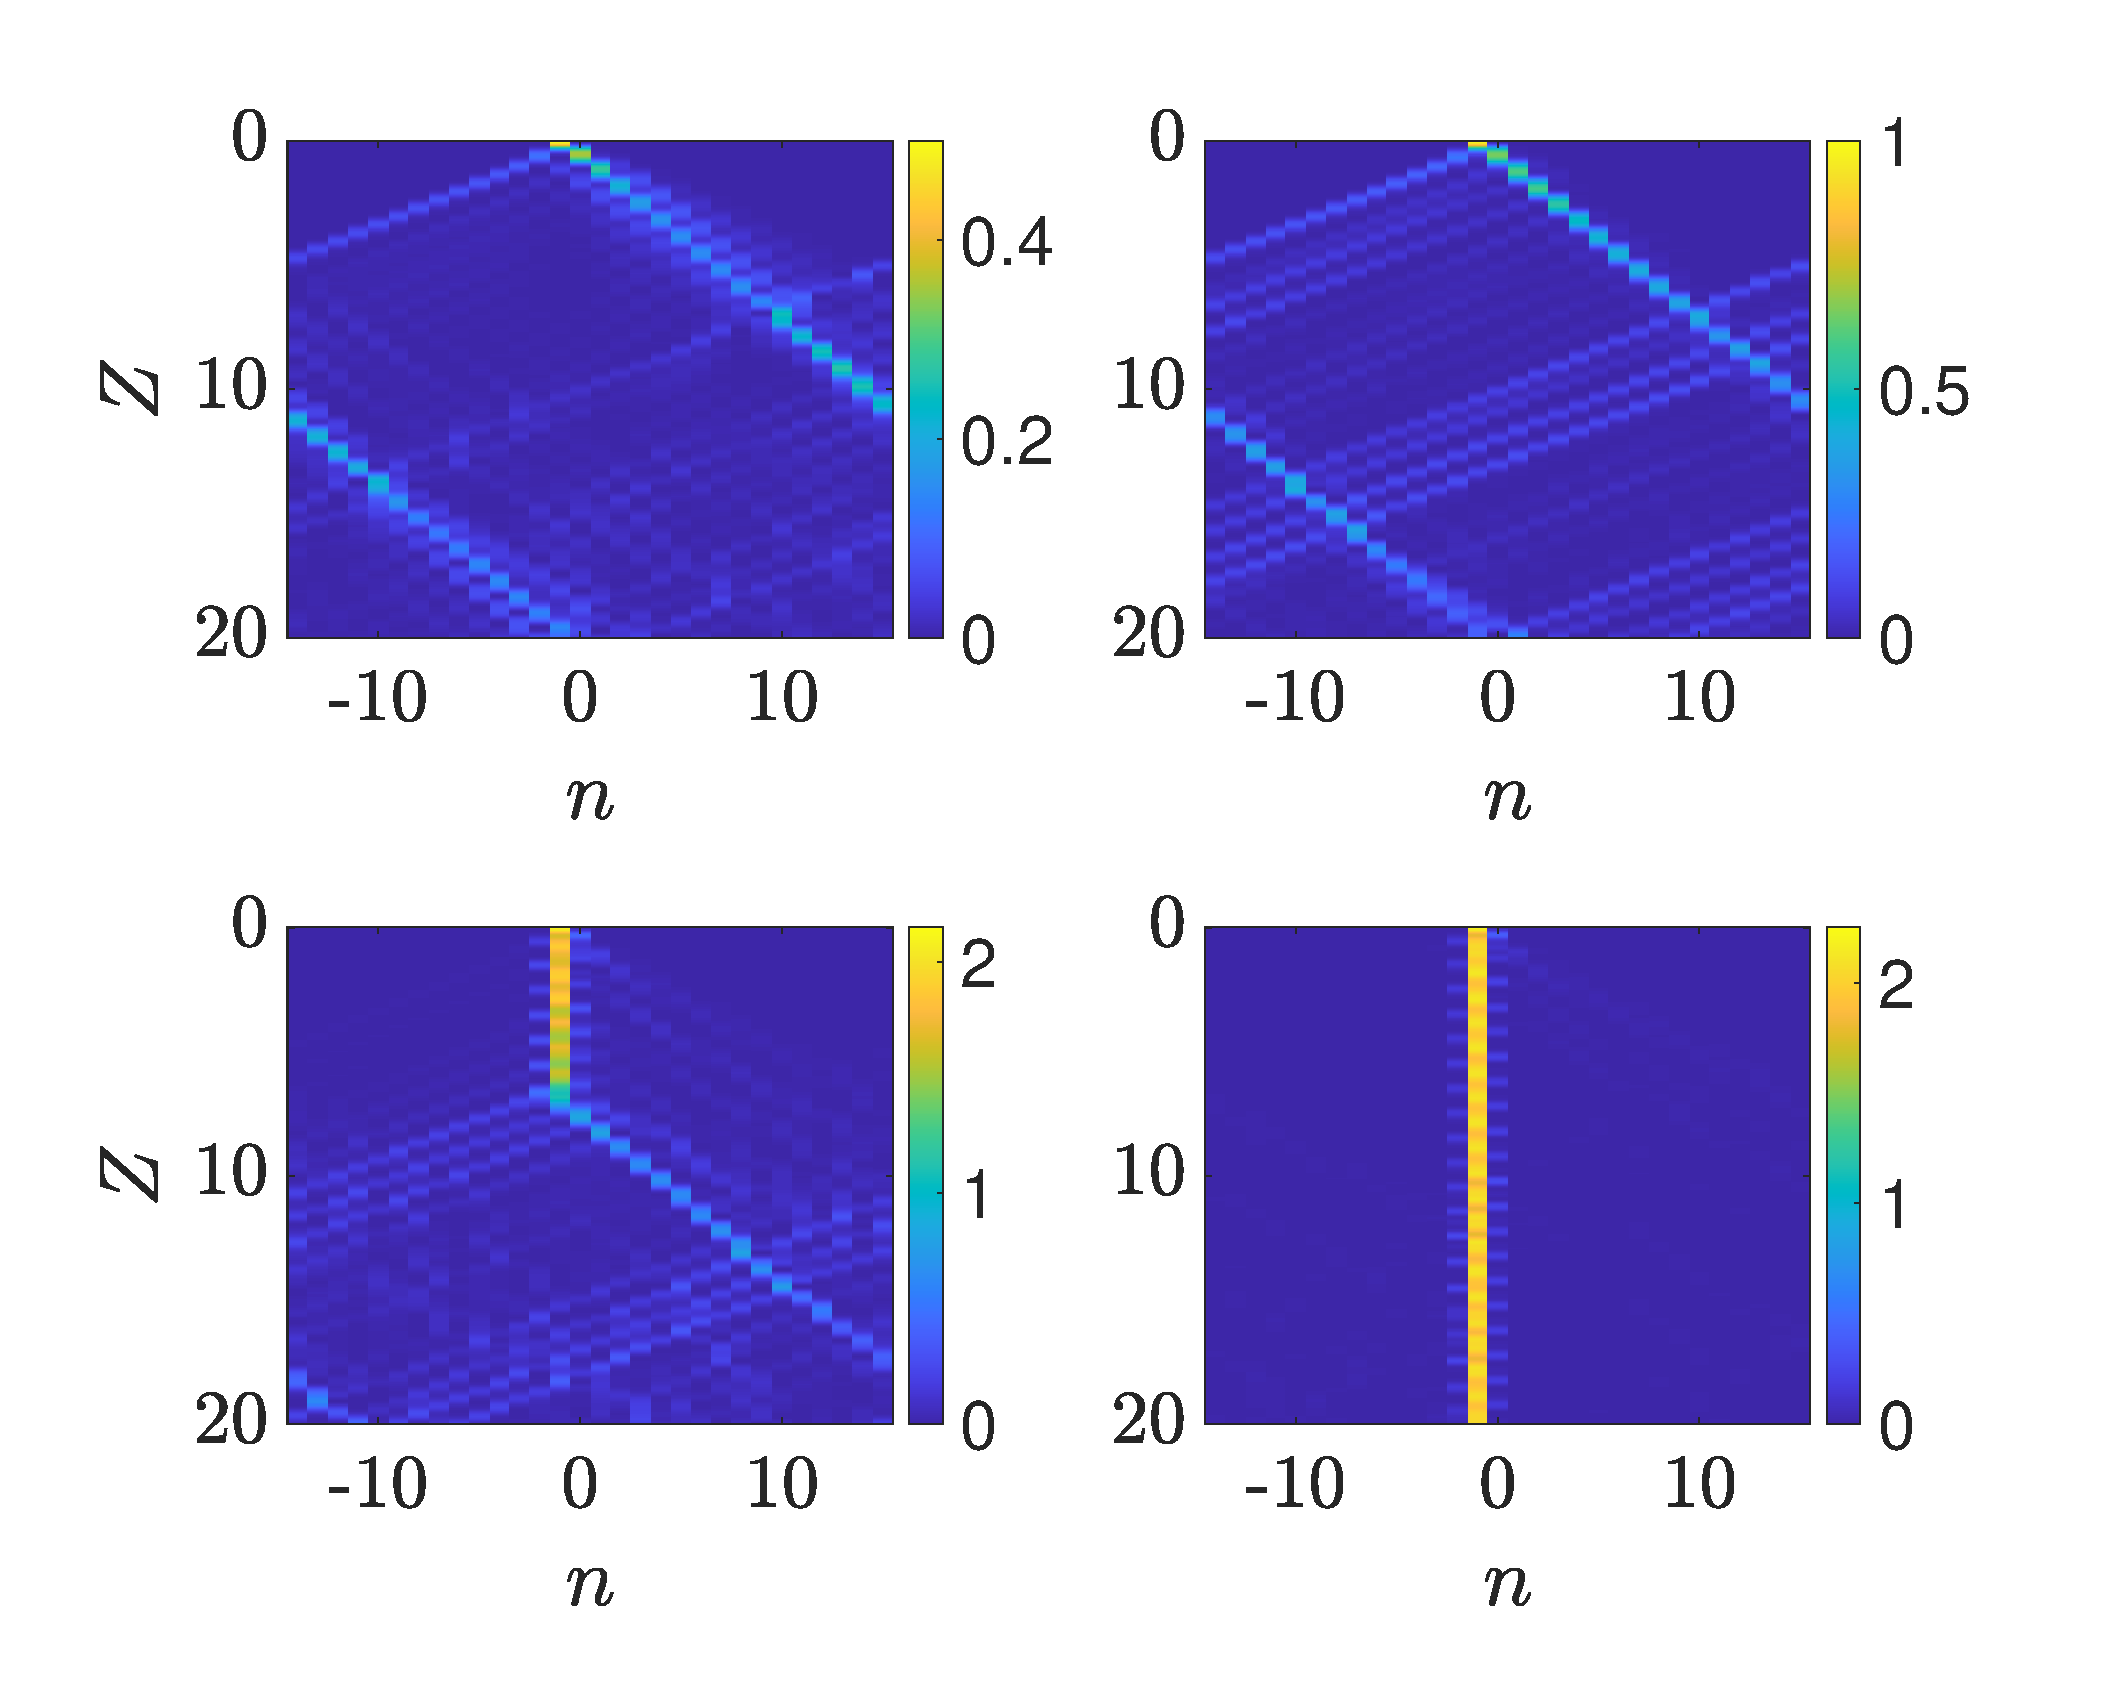
\includegraphics[width=9cm]{timestep-1.eps}
    \caption{Colormap showing the density of the solution of equation \cref{eq:modelZ} evolving in $Z$, starting with a single excited site at $n=-1$ with power $P=0.5,1,2.15,2.25$ (left to right, top to bottom).}
    \label{fig:timestep-1}
\end{figure}

\subsection{Simplified model}\label{sec:simplified}

A further heuristic and qualitative, yet in our view informative and intuitive explanation of these different behaviors can be obtained by considering the simplification of the system \cref{eq:model} obtained by approximating the coupling functions $J_n(Z)$ with step functions, as is done, e.g.,
in the setting of the Kronig-Penney model~\cite{kronig}. 
Notice that such a perspective has also been beneficial in
a quantitative
fashion in the past in the context of nonlinearity (rather than dispersion)
management in works such as~\cite{PhysRevLett.97.033903,PhysRevLett.97.234101}.
Specifically, we define % JCM: shouldn't it be $n (mod 3)\equiv 1$ instead of $n\equiv 1 (mod 3)$?
\begin{equation}\label{eq:simpleJn}
J_n(Z) = \begin{cases}
C\chi_{[0,1/3]}(Z) & n \equiv 2 \text{ (mod 3)} \\
C\chi_{[1/3,2/3]}(Z) & n \equiv 1 \text{ (mod 3)}\\
C\chi_{[2/3,1]}(Z) & n \equiv 0 \text{ (mod 3)}
\end{cases}
\end{equation}
for $Z \in [0,1]$, and extend periodically for all $Z$ (\cref{fig:Jsimple}). The function $\chi_{[a,b}](Z)$ is the characteristic function of the interval $[a,b]$, defined by
\[
\chi_{[a,b]}(Z) = \begin{cases}
1 & Z \in [a,b] \\
0 & \text{otherwise}.
\end{cases}
\]
\begin{figure}
    \centering
    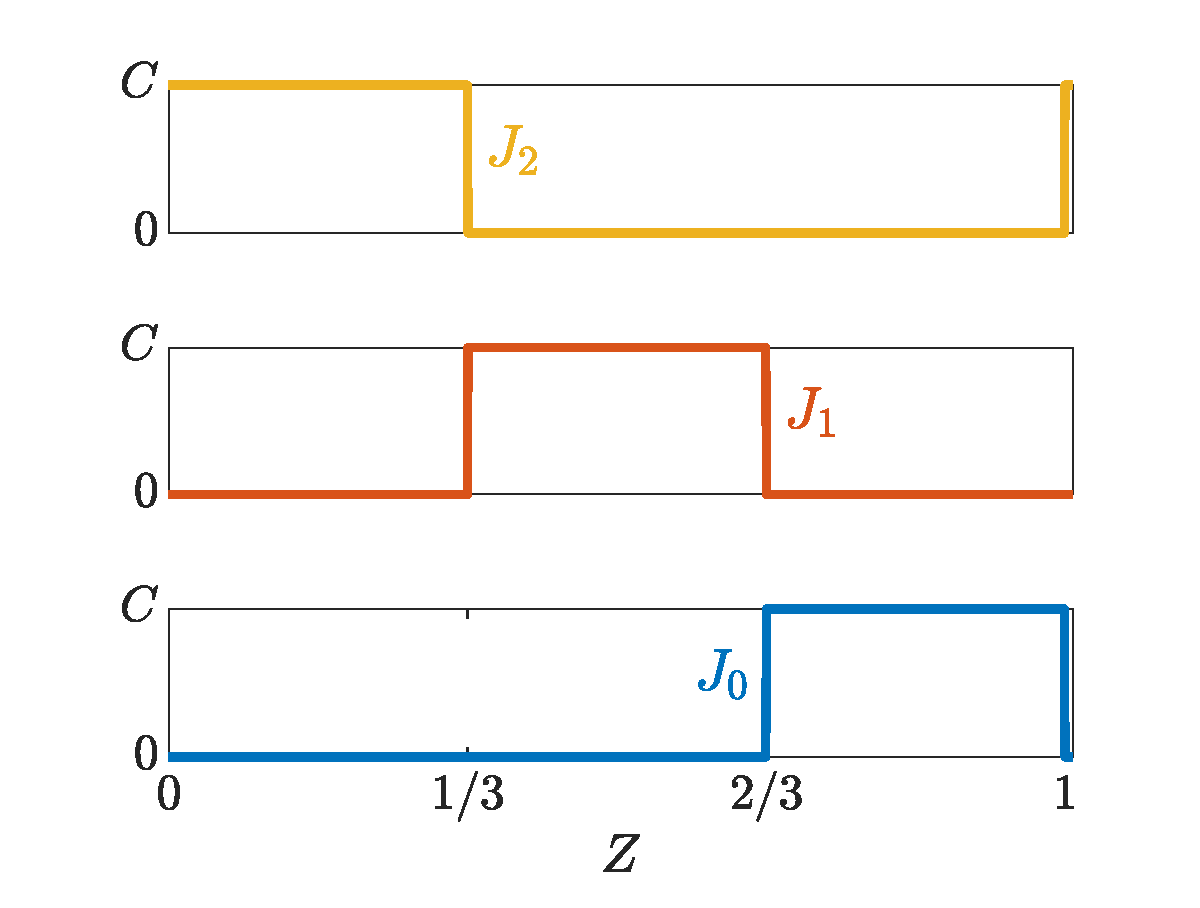
\includegraphics[width=8cm]{Jsimple.eps}
    \caption{Simplified coupling functions \cref{eq:simpleJn} for $Z \in [0,1]$.}
    \label{fig:Jsimple}
\end{figure}

Using this approximation, on the interval $Z \in [0, 1/3]$, the only coupling is between the sites $n \equiv0\,(\text{mod}\,3)$ and their left neighbors, which effectively creates a string of independent dimers. Looking only at the sites $n=0$ and $n=-1$, i.e., one of these dimers, and following the analysis in \cite{Kenkre1986}, the system of equations \cref{eq:powerevol} reduces to 
\begin{equation}\label{eq:powerevolsimple}
\begin{aligned}
\frac{d\rho_{0,0}}{dZ} &= iLC \left( \rho_{-1,0} - \rho_{0,-1} \right) \\
\frac{d\rho_{-1,-1}}{dZ}  &= iLC \left( \rho_{0,-1} - \rho_{-1,0} \right) \\
\frac{d\rho_{-1,0} }{dZ} &= iL \big[ C(\rho_{0,0} - \rho_{-1,-1}) \\
&\qquad + g ( \rho_{-1,-1} - \rho_{0,0}) \rho_{-1,0} \big] \\
\frac{d\rho_{0,-1}}{dZ}  &= iL \big[ C(\rho_{-1,-1} - \rho_{0,0}) \\
&\qquad + g ( \rho_{0,0} - \rho_{-1,-1} ) \rho_{0,-1} \big].\\
\end{aligned}
\end{equation}
Let $p = \rho_{0,0} - \rho_{-1,-1}$ be the difference between the powers of site $n=0$ and site $n=1$. In addition, as in \cite{Kenkre1989}, we define $q = i(\rho_{-1,0} - \rho_{0,-1})$ and $r = \rho_{-1,0} - \rho_{0,-1}$. Using \cref{eq:powerevolsimple}, we obtain the equations
\begin{align}
\frac{dp}{dZ} &= 2LCq \label{eq:peq}\\
\frac{dq}{dZ} &= -L(2Cp - gpr) \label{eq:qeq}\\
\frac{dr}{dZ} &= -Lgpq. \label{eq:req}
\end{align}
Since
\[
\frac{d}{dZ}p^2 = 2p \frac{dp}{dZ} = 4Lcpq,
\]
equation \cref{eq:req} becomes
\[
\frac{dr}{dZ} = -\frac{g}{4C}\frac{d}{dZ}p^2,
\]
which has solution
\begin{equation}\label{eq:rsol}
r = r_0 - \frac{g}{4C}\left( p^2 - p_0^2 \right),
\end{equation}
where $r_0$ and $p_0$ are the initial conditions at $Z=0$. Differentiating \cref{eq:peq}, substituting \cref{eq:qeq} and the solution \cref{eq:rsol}, we obtain the second-order differential equation for $p$
\begin{equation}\label{eq:pode}
\begin{aligned}
\frac{d^2p}{dZ^2} &= L^2 \left( A p - B p^3 \right) \\
A &= -4C^2 + 2Cgr_0 + \frac{g^2}{2}p_0^2
\qquad\quad B = \frac{g^2}{2}.
\end{aligned}
\end{equation}

We are interested in the case of a single-site initial condition of power $P$ at site $n=0$, for which $p_0 = P$ and $r_0 = 0$. Following \cite{Kenkre1986}, for fixed $C$ and $g$, equation \cref{eq:pode} has an exact solution
\begin{equation}\label{eq:psol}
p(Z) =
\begin{cases}
P\,\text{cn}\left(2CLZ ; k=\dfrac{g P}{4C} \right) & P < P^*\\
P\,\text{dn}\left(\dfrac{g P L}{2}Z ; k=\dfrac{4C}{g P} \right) & P > P^*,
\end{cases}
\end{equation}
where the critical power $P^*$ is given by
\begin{equation}\label{eq:pstar}
P^* = \dfrac{4C}{g}.
\end{equation}
The functions $\text{cn}(z ; k)$ and $\text{dn}(z ; k)$ are the Jacobi elliptic functions with elliptic modulus $k$ (we note that these are often written in terms of the elliptic parameter $m$, where $m = k^2$). Since the total power is conserved, i.e. $|u_0(Z)|^2 + |u_{-1}(Z)|^2 = P$ for all $Z$ in the above interval, 
% Comment: this is still valid ONLY between 0 and 1/3. OK?
the power at sites $n=0$ and $n=-1$ is then given by
\begin{equation}\label{eq:u0u-1}
\begin{aligned}
|u_0(Z)|^2 &= \frac{1}{2}\left( P + p(Z) \right)\\
|u_{-1}(Z)|^2 &= \frac{1}{2}\left( P - p(Z) \right).
\end{aligned}
\end{equation}

There are two fundamental behaviors of the single-site initial condition in the simplified model, depending on whether $P < P^*$ or $P > P^*$. In the dimer, a sharp transition between the two behaviors occurs at $P = P^*$ (see \cite{Kenkre1986}). We note that this transition is somewhat blurred in this model, even with the simplified coupling function, since the initial dimer coupling is broken at $Z=1/3$.

\subsubsection{\texorpdfstring{Case 1: $P < P^*$}{Case 1: P < Pstar}}

For $P < P^*$, the solution $p(Z)$ involves the Jacobi cn function, which oscillates about 0 with period $2K(k)/CL$, where
\begin{equation}\label{eq:Kellipticint}
K(k) = \int_0^{\pi/2} \frac{d\theta}{\sqrt{1-k^2 \sin^2 \theta}}
\end{equation}
is the complete elliptic integral of the first kind. The period of oscillation becomes infinite as $P$ approaches $P^*$ from below.
As a consequence, the intensity $|u_0|^2$, given by equation \cref{eq:u0u-1}, exhibits large amplitude oscillations with this period from 0 to $P$, centered at $P/2$ (\cref{fig:simplemodel1}, left).
Power initially flows to the left; if the coupling is not cut off at $Z=1/3$ (and no other couplings are activated), there is a critical value $Z_1^*$ of $Z$ at which the power from site $n=0$ has been completely transferred to site $n=-1$; after this point, the power starts flowing back in the other direction. This critical value $Z_1^*$ is larger for larger starting power $P$ (see \cref{fig:simplemodel1}, left).
For most configurations, including all of the examples in \cref{fig:simplemodel1}, $Z_1^* > 1/3$, thus there is still power remaining in site 0 when the coupling switches off at $Z=1/3$. The left panel of \cref{fig:powertransfer} plots the fraction of power transferred from site $n=0$ to site $n=-1$ at $Z=1/3$ as the starting power varies. If this fraction is close to 1, numerical evolution experiments find leftward-moving solutions starting from a single-site initial condition (see the first three panels of \cref{fig:timestepsimplebelowpstar}). As the initial power $P$ approaches $P^*$ from below, the fraction of power transferred at $Z=1/3$ decreases to approximately 0.5, and we do not expect to see pure leftward-moving solutions. Numerical evolution experiments show that the initial power splits into a leftward and a rightward moving solution (bottom right panel of \cref{fig:timestepsimplebelowpstar}).
%For large enough enough power $P$, it is no longer possible
%to transfer the power from $n=0$ to $n=-1$. Rather, in this setting,
%the $n=0$ site experiences the self-trapping transition with the
%relevant intensity oscillating close(r for larger $P$) to its initial
%value. This is shown in the right panel of Figure \cref{fig:simplemodel1}.
%Accordingly, the right panel of Figure \cref{fig:powertransfer} shows
%that in this case the power remains trapped at the original site,
%ultimately leading to localized (self-trapped) states.

We note that it is possible to choose parameters so that, for the simplified model, the period of $p(Z)$ is 2/3, i.e. $Z_1^* = 1/3$, so that power has been completely transferred from $n=0$ to $n=-1$ when the coupling switches off. The next coupling is between $n=-1$ and $n=-2$ for $Z \in [1/3,2/3]$. This pattern continues, and for this choice of parameters, the simplified model supports 
a(n exact) leftward-moving solution which persists for a large interval in $Z$ (\cref{fig:simplemodel1}, 
(\cref{fig:simplecomplete}, top). % JCM: the reference to the figure is wrong; but I don't know what is the right one
A comparison between the evolution of the original and simplified systems from single-site initial conditions is shown in the top panel of \cref{fig:simplecompare}. We will see below in \cref{sec:movingsol} that left-moving coherent structures exist in the full model, but these do not have pure single-site initial conditions. We also note that by symmetry of \cref{eq:powerevolsimple}, a similar analysis holds for rightward-moving solutions starting with single-site initial conditions at $n=-1$ on the interval $Z \in [0,1/3]$. The general behavior of the rightward-moving solution is discussed in \cref{sec:singlesite}.

\begin{figure}
    \centering
    \begin{tabular}{cc}
    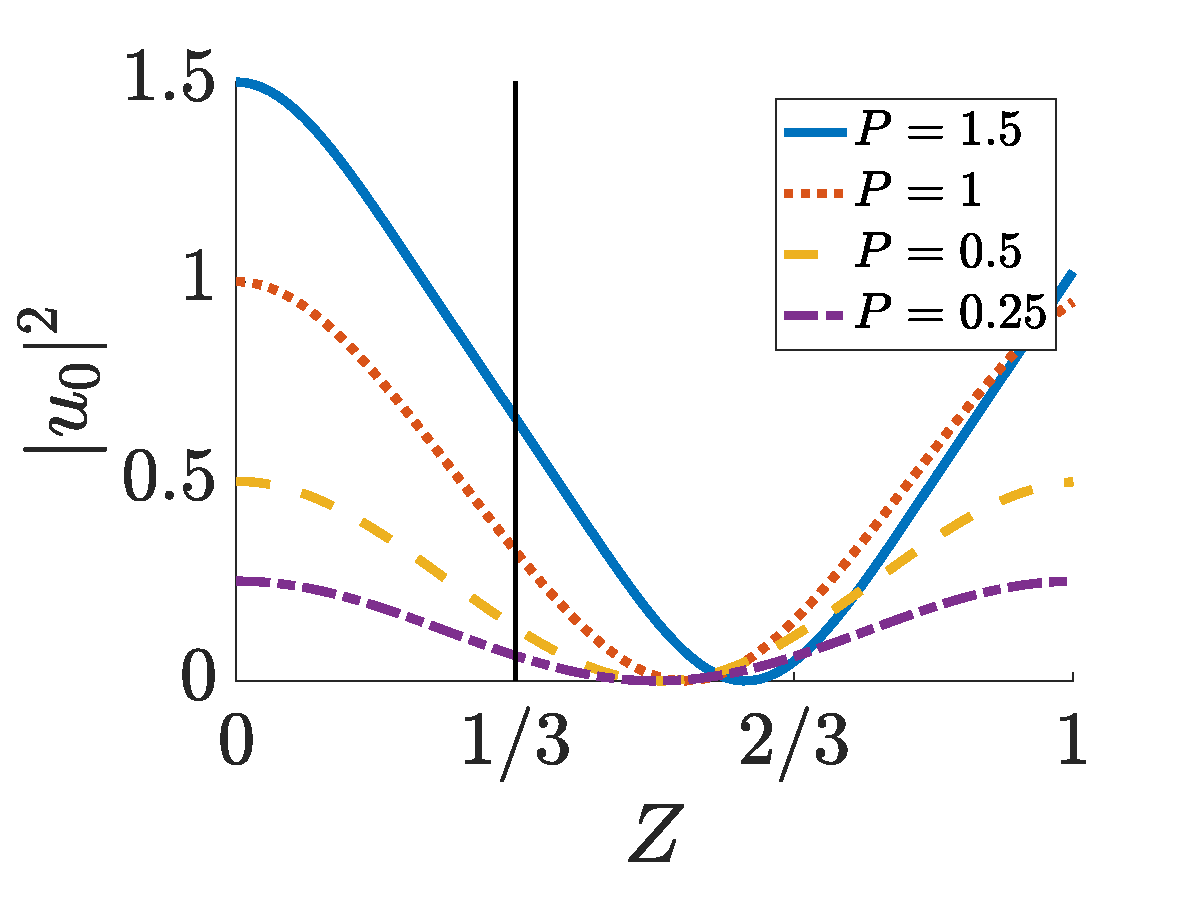
\includegraphics[width=4cm]{plotCN.eps} &
    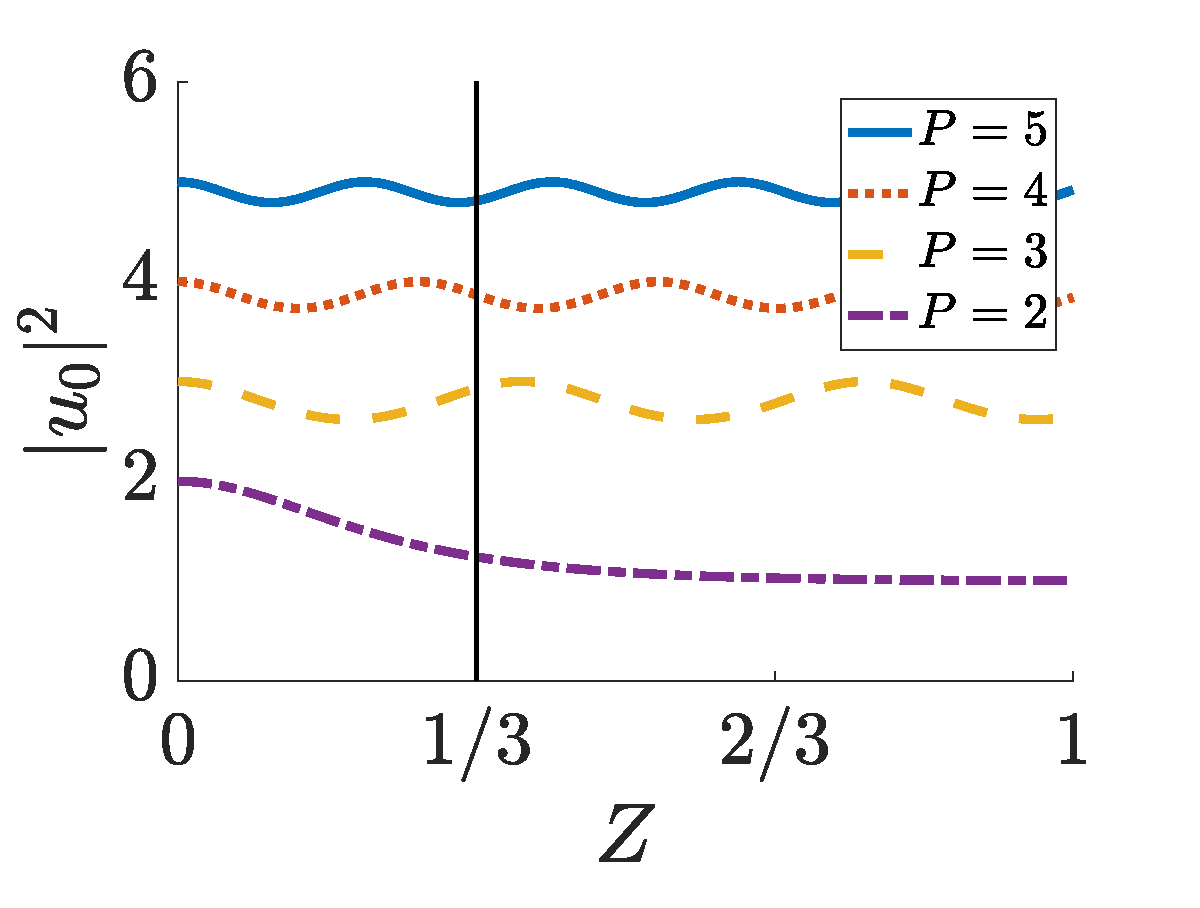
\includegraphics[width=4cm]{plotDN.eps}
    \end{tabular}
    \caption{Plot of $|u_0|^2$ in simplified model, given by \cref{eq:u0u-1}, vs. $Z$ for initial power $P<P^*$ (left) and $P>P^*$ (right). Although this solution only holds for $Z \in [0, 1/3]$ ($Z=1/3$ is marked with a solid vertical line), it is continued to $Z=1$ for illustrative purposes. $C=0.5$, $g=1$, $P^* = 2$.}
    \label{fig:simplemodel1}
\end{figure}

\begin{figure}
    \centering
    \begin{tabular}{cc}
    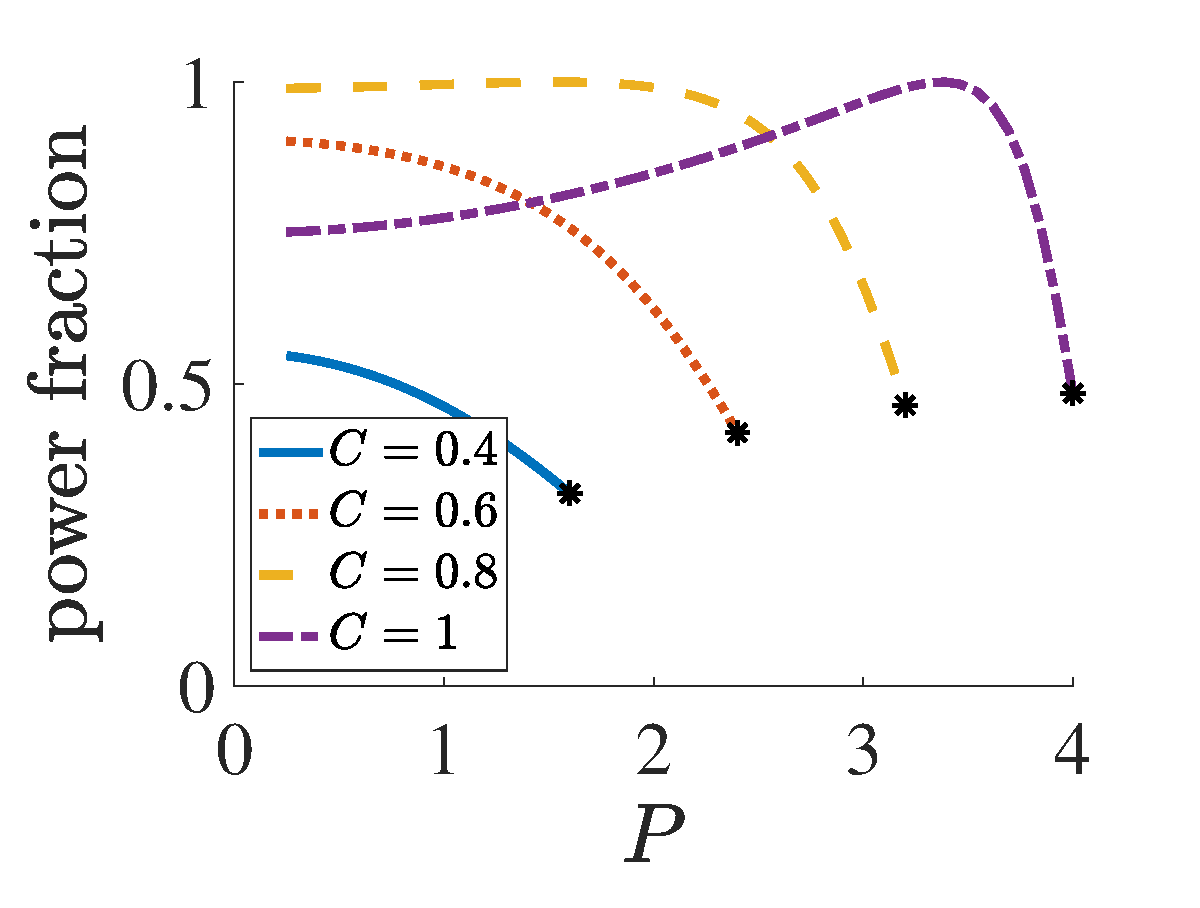
\includegraphics[width=4cm]{powerfractransfer} &
    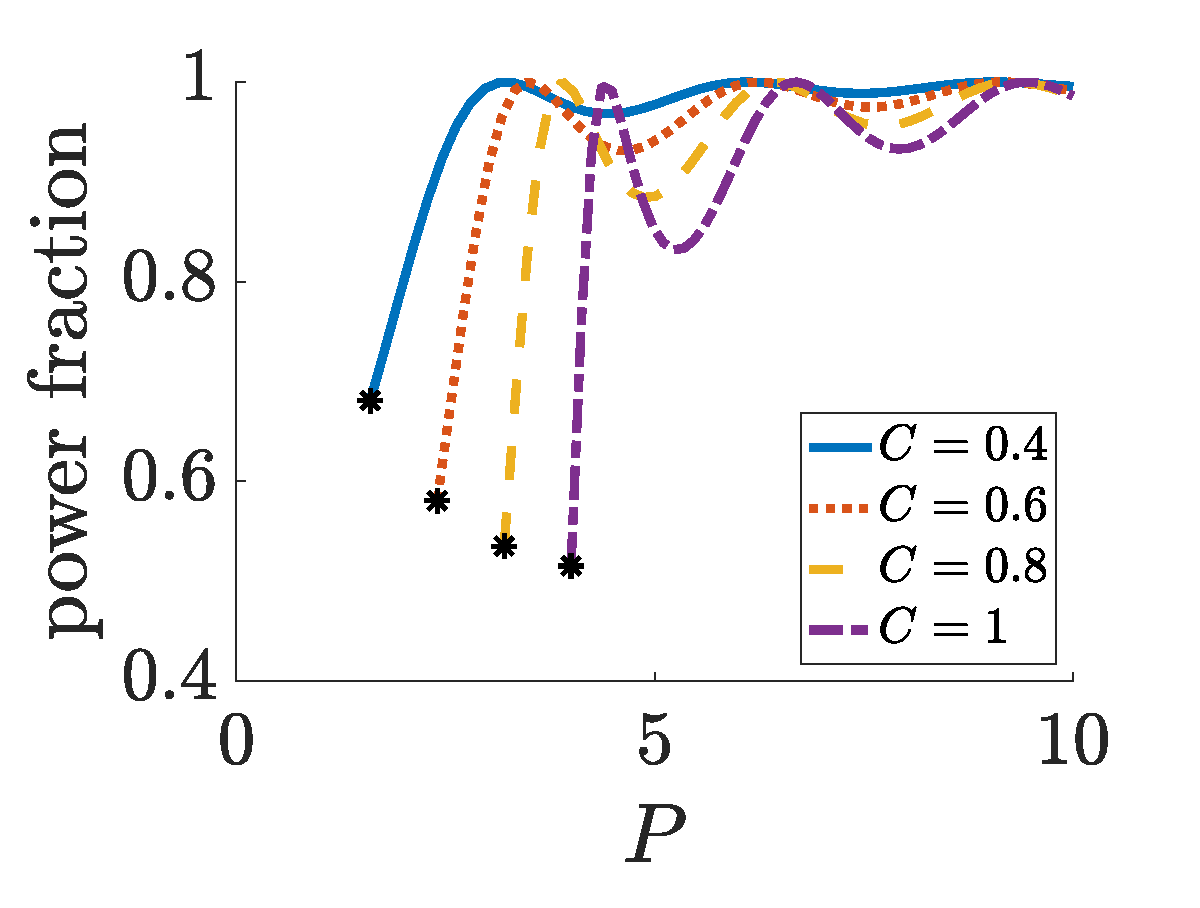
\includegraphics[width=4cm]{powerfracremain.eps}
    \end{tabular}
    \caption{Fraction of power transferred from site $n=0$ to site $n=-1$ at $Z=1/3$ for $P<P^*$ for varying $C$ (left). Fraction of power remaining at site $n=0$ at $Z=1/3$ for $P>P^*$ for varying $C$ (right). For each curve, $P^*$ is indicated with a star. $g=1$.}
    \label{fig:powertransfer}
\end{figure}

\begin{figure}
    \centering
    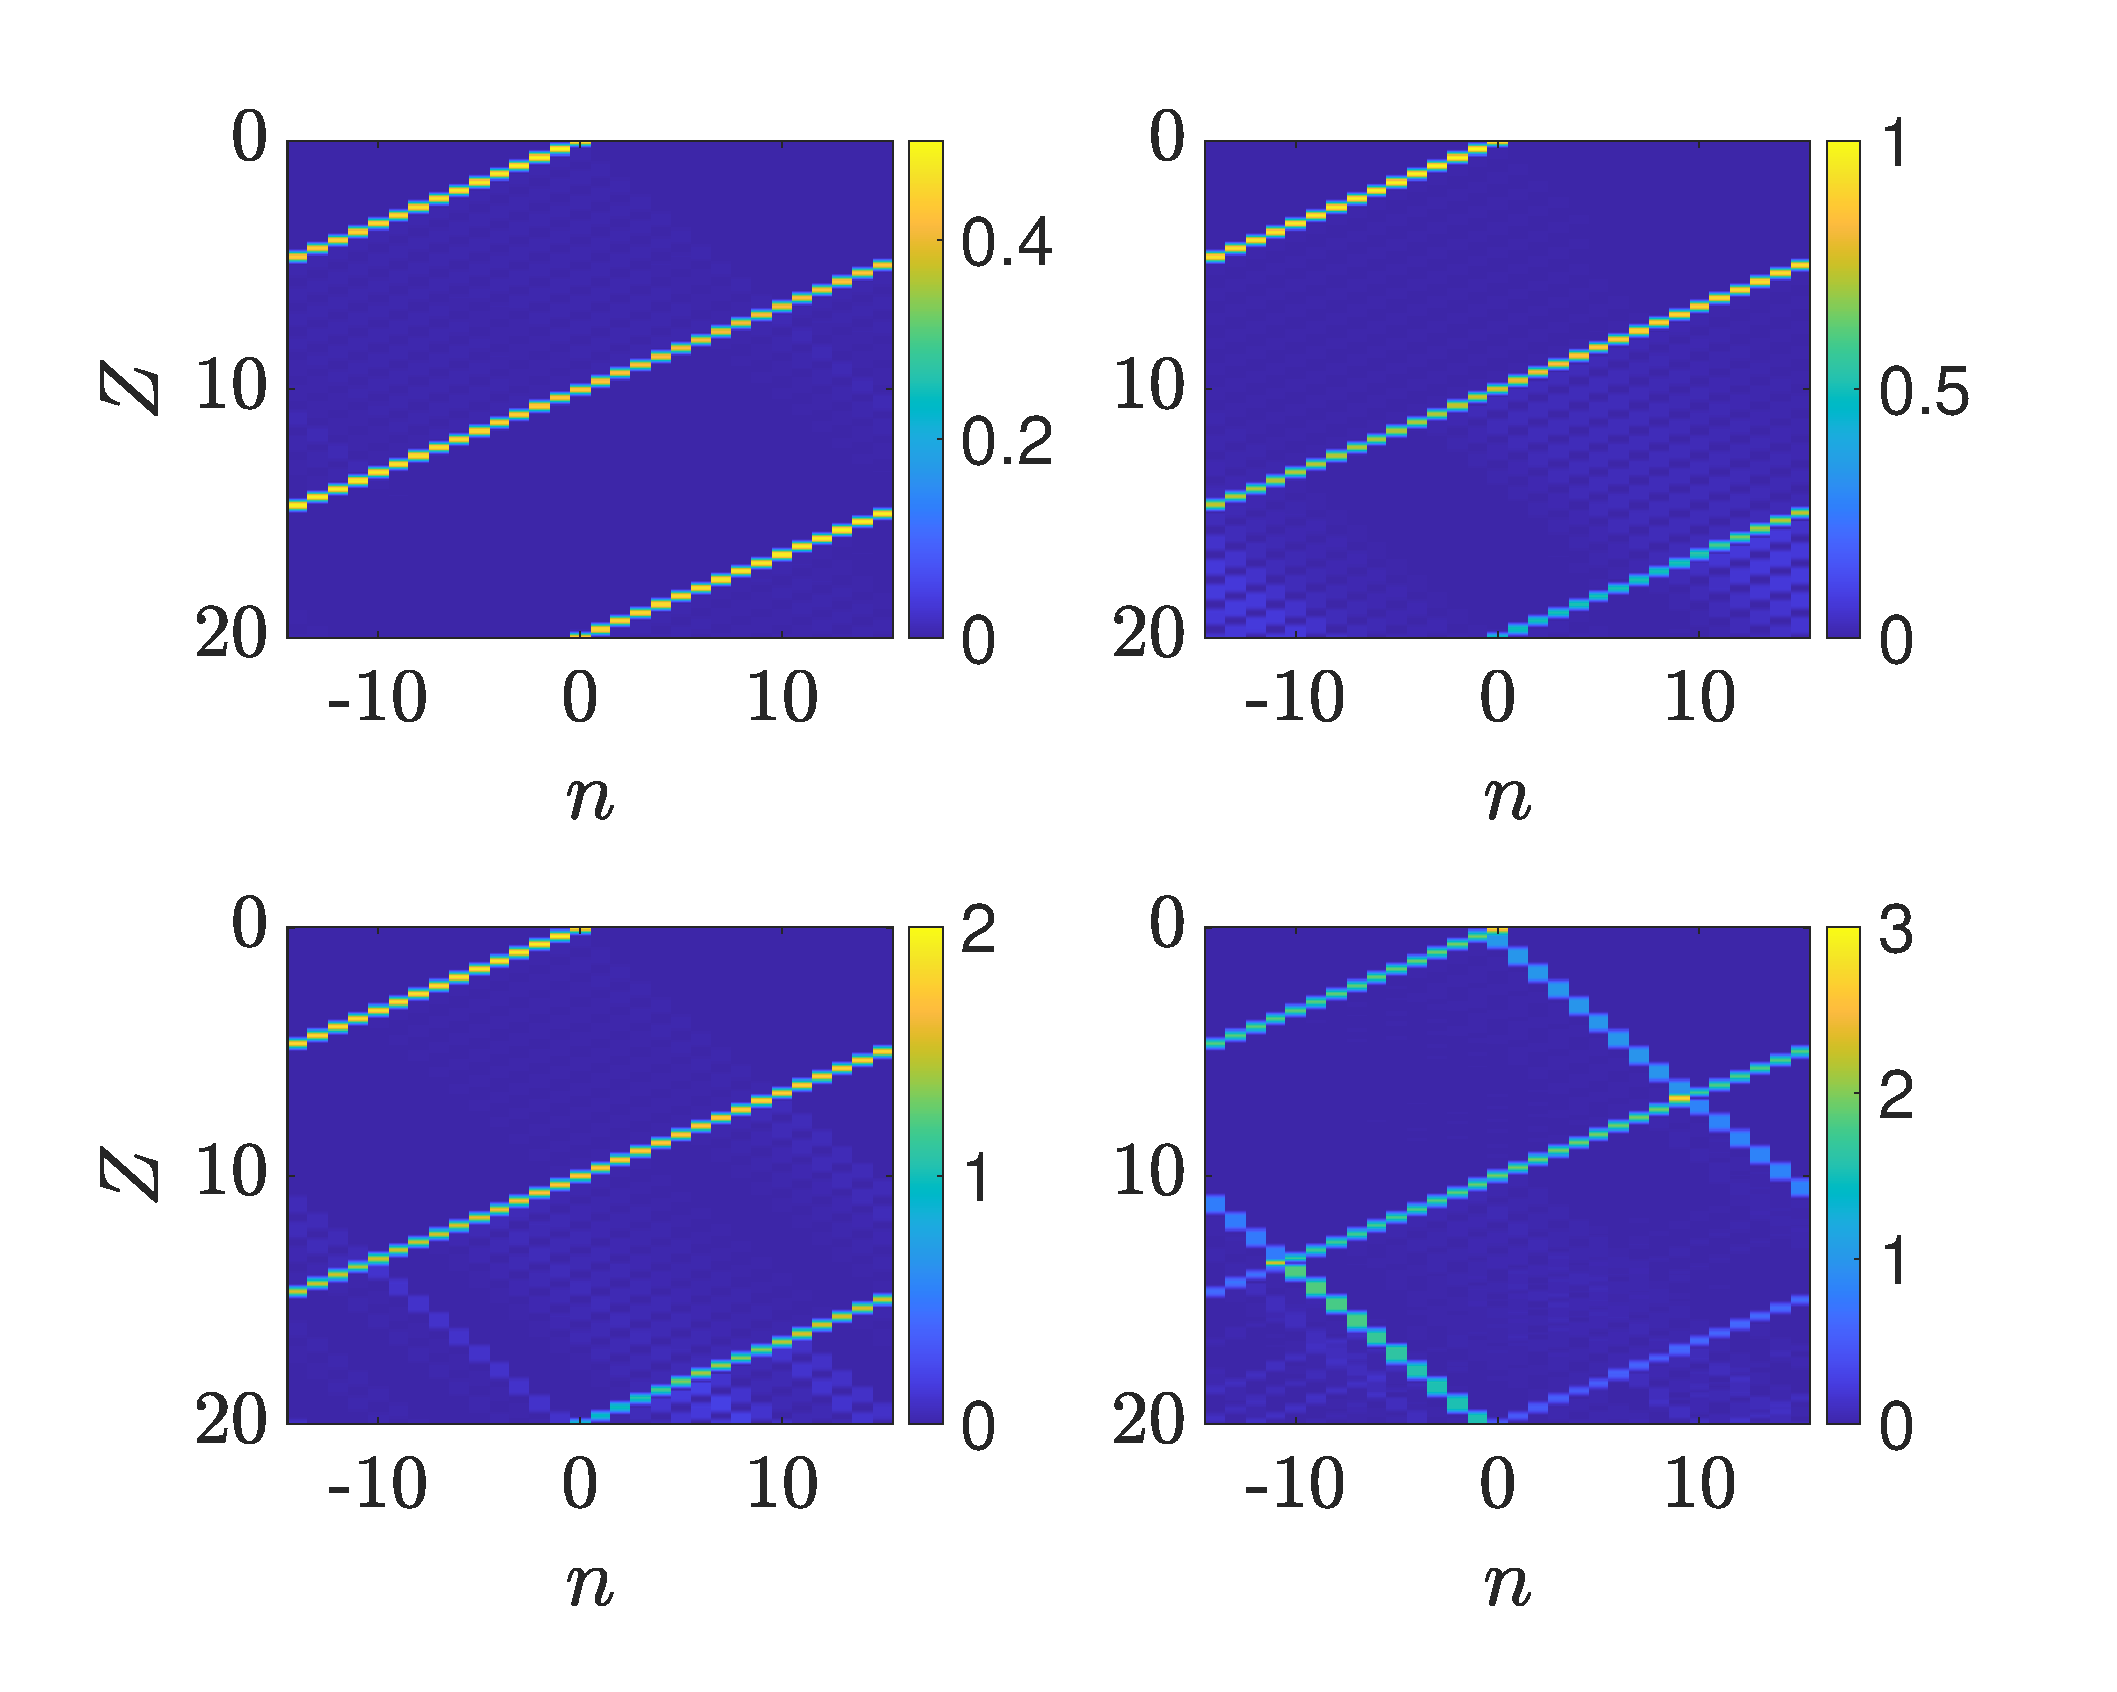
\includegraphics[width=9cm]{timestepsimplebelowpstar.eps}
    \caption{Colormap showing power of solution of equation \cref{eq:modelZ} with simplified coupling function \cref{eq:simpleJn} evolving in $Z$, starting with a single excited site at $n=0$ with power $P=0.5,1,2,3$, $P<P^*$ (left to right, top to bottom). Fraction of power transferred from site $n=0$ to site $n=-1$ at $Z=1/3$ is 0.9910, 0.9959, 0.9909, 0.6636 (respectively). $P^*=3.2$, $C=0.8$, $g=1$.}
    \label{fig:timestepsimplebelowpstar}
\end{figure}

\begin{figure}
    \centering
    \begin{tabular}{ccc}
    \includegraphics[width=2.5cm]{sLcomp05} &
    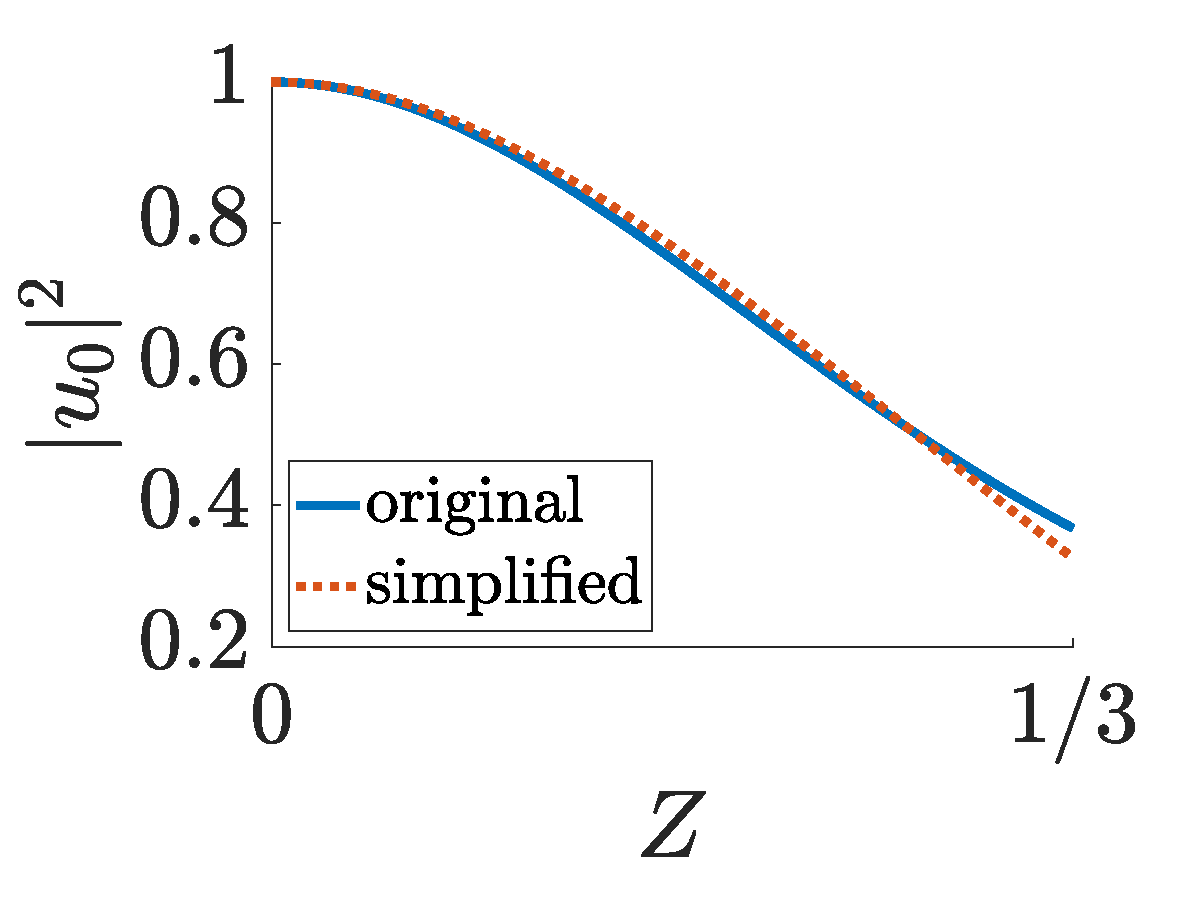
\includegraphics[width=2.5cm]{sLcomp1}  &
    \includegraphics[width=2.5cm]{sLcomp15} \\
    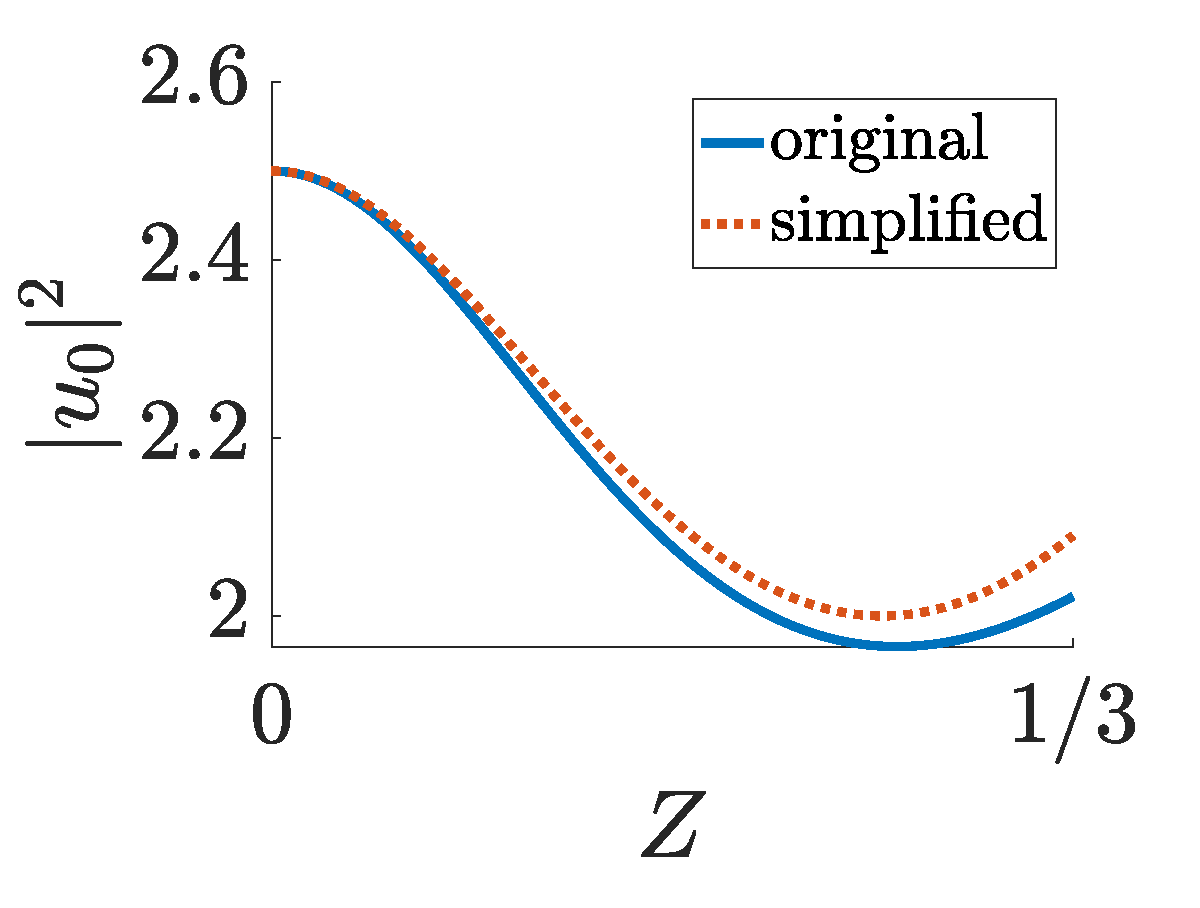
\includegraphics[width=2.5cm]{sscomp25} &
    \includegraphics[width=2.5cm]{sscomp35}  &
    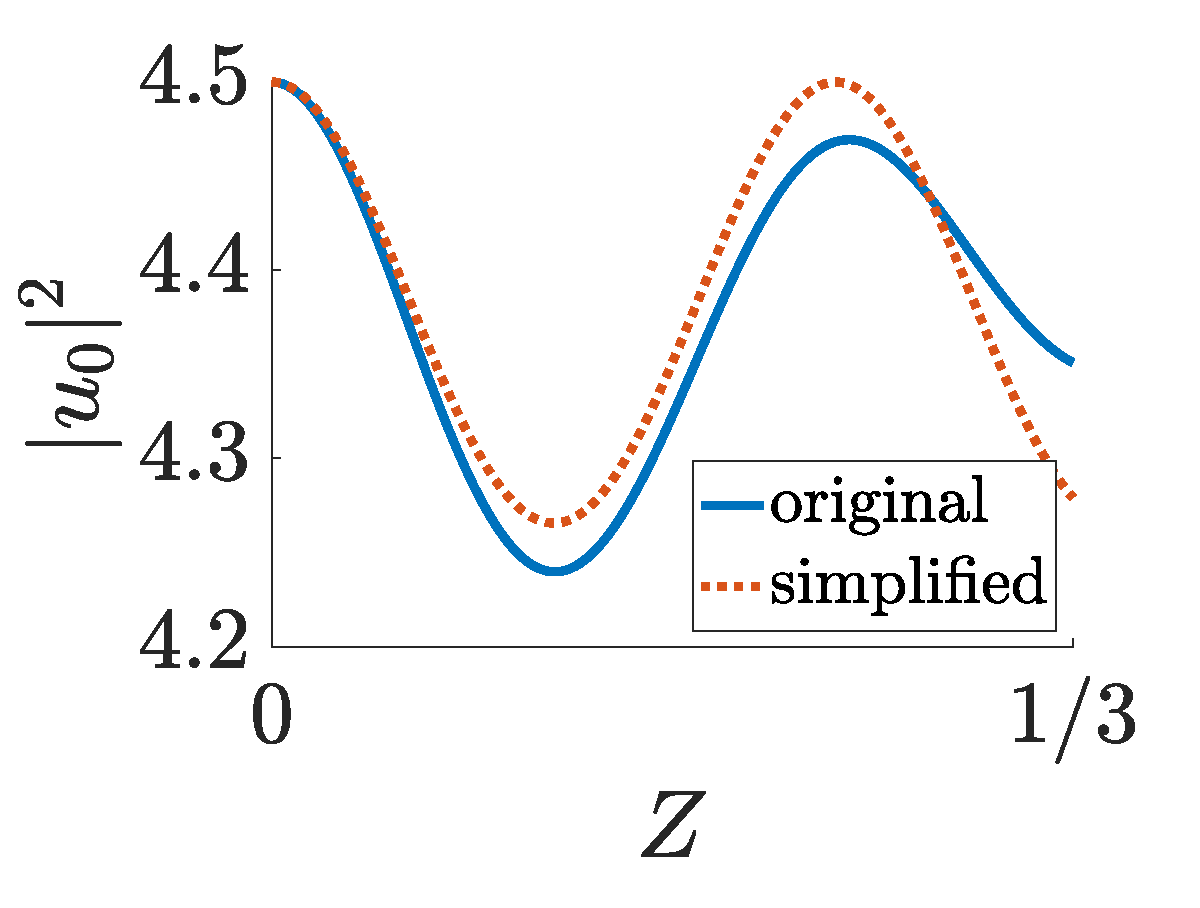
\includegraphics[width=2.5cm]{sscomp45}
    \end{tabular}
    \caption{Power $|u_0|^2$ of site $n=0$ on $Z\in[0,1/3]$ for $P<P^*$ (top, $P=0.5$, $1$, and $1.5$), and $P>P^*$ (bottom, $P=2.5$, $3.5$, and $4.5$) for original system (solid blue line) and simplified system (dotted orange line). $C=0.5$, $g=1$, $P^* = 2$.}
    \label{fig:simplecompare}
\end{figure}

\begin{figure}
    \centering
    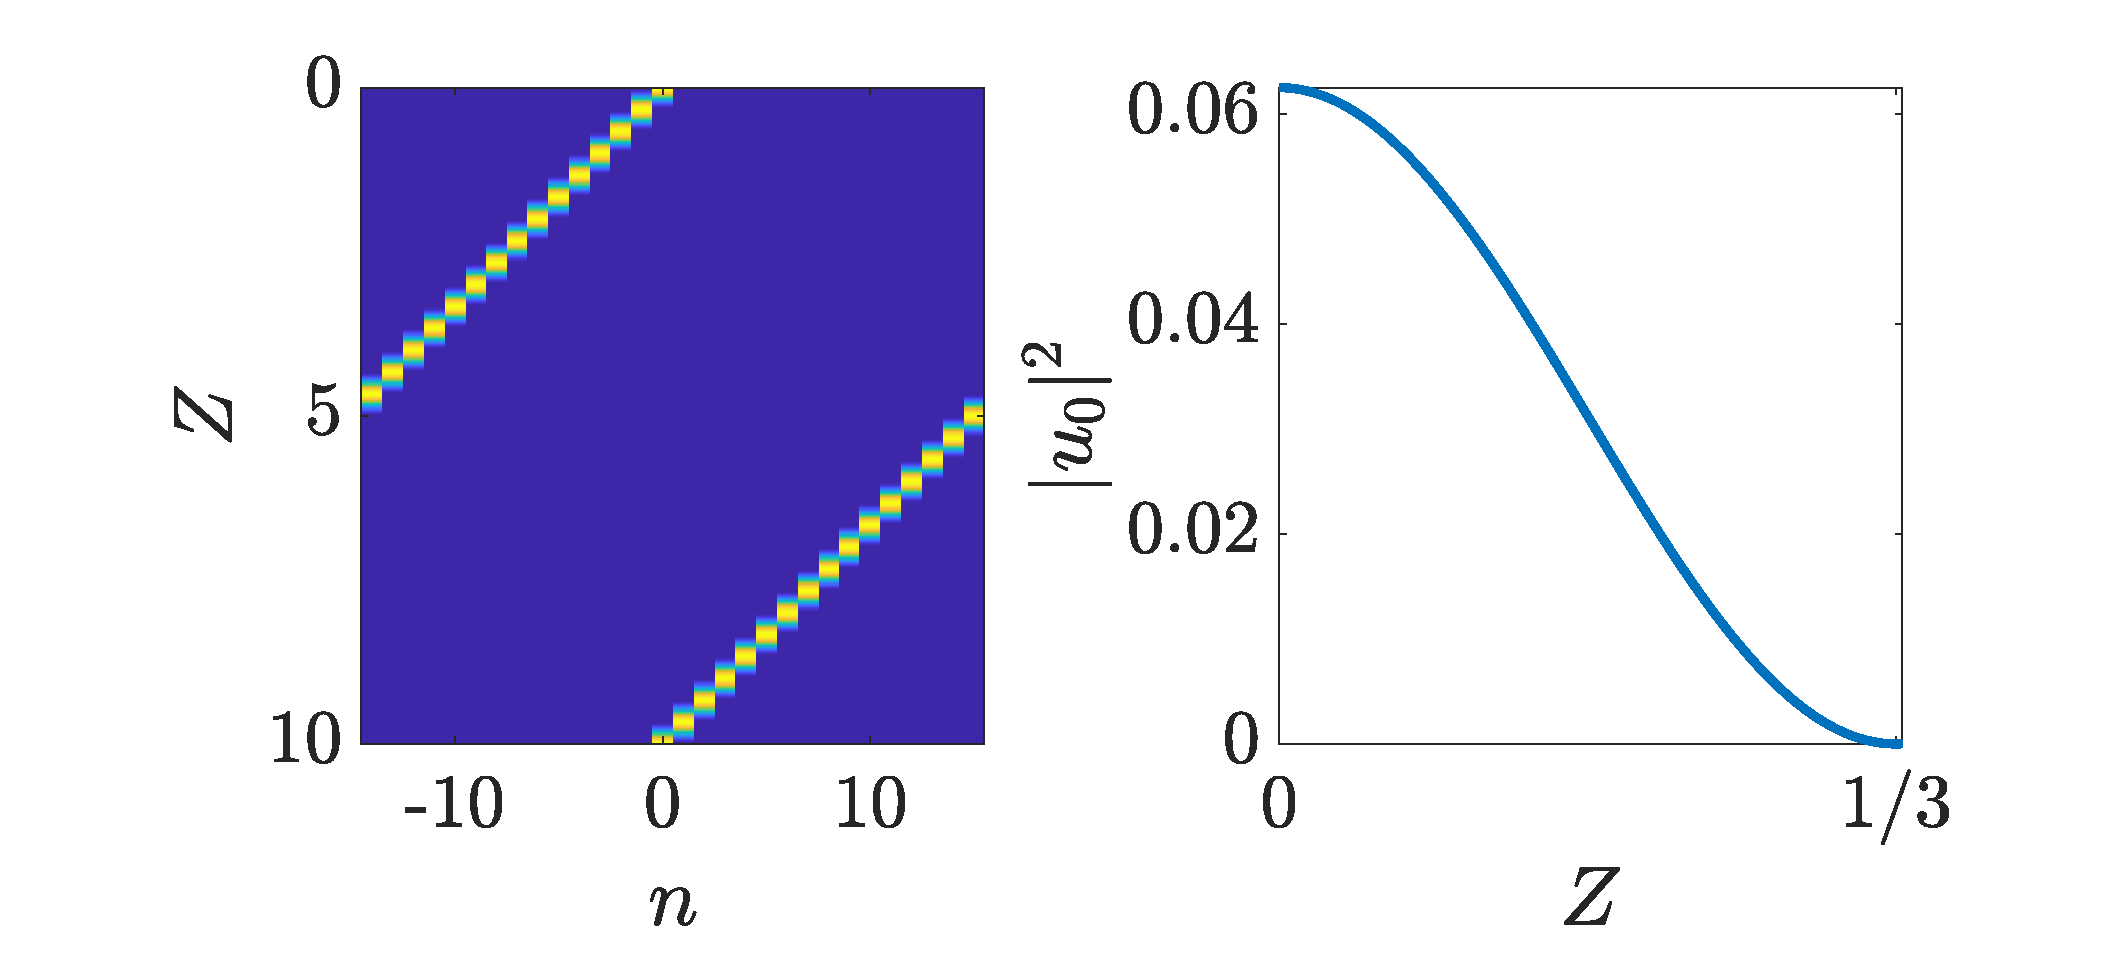
\includegraphics[width=9cm]{leftsimplifiedcomplete}
    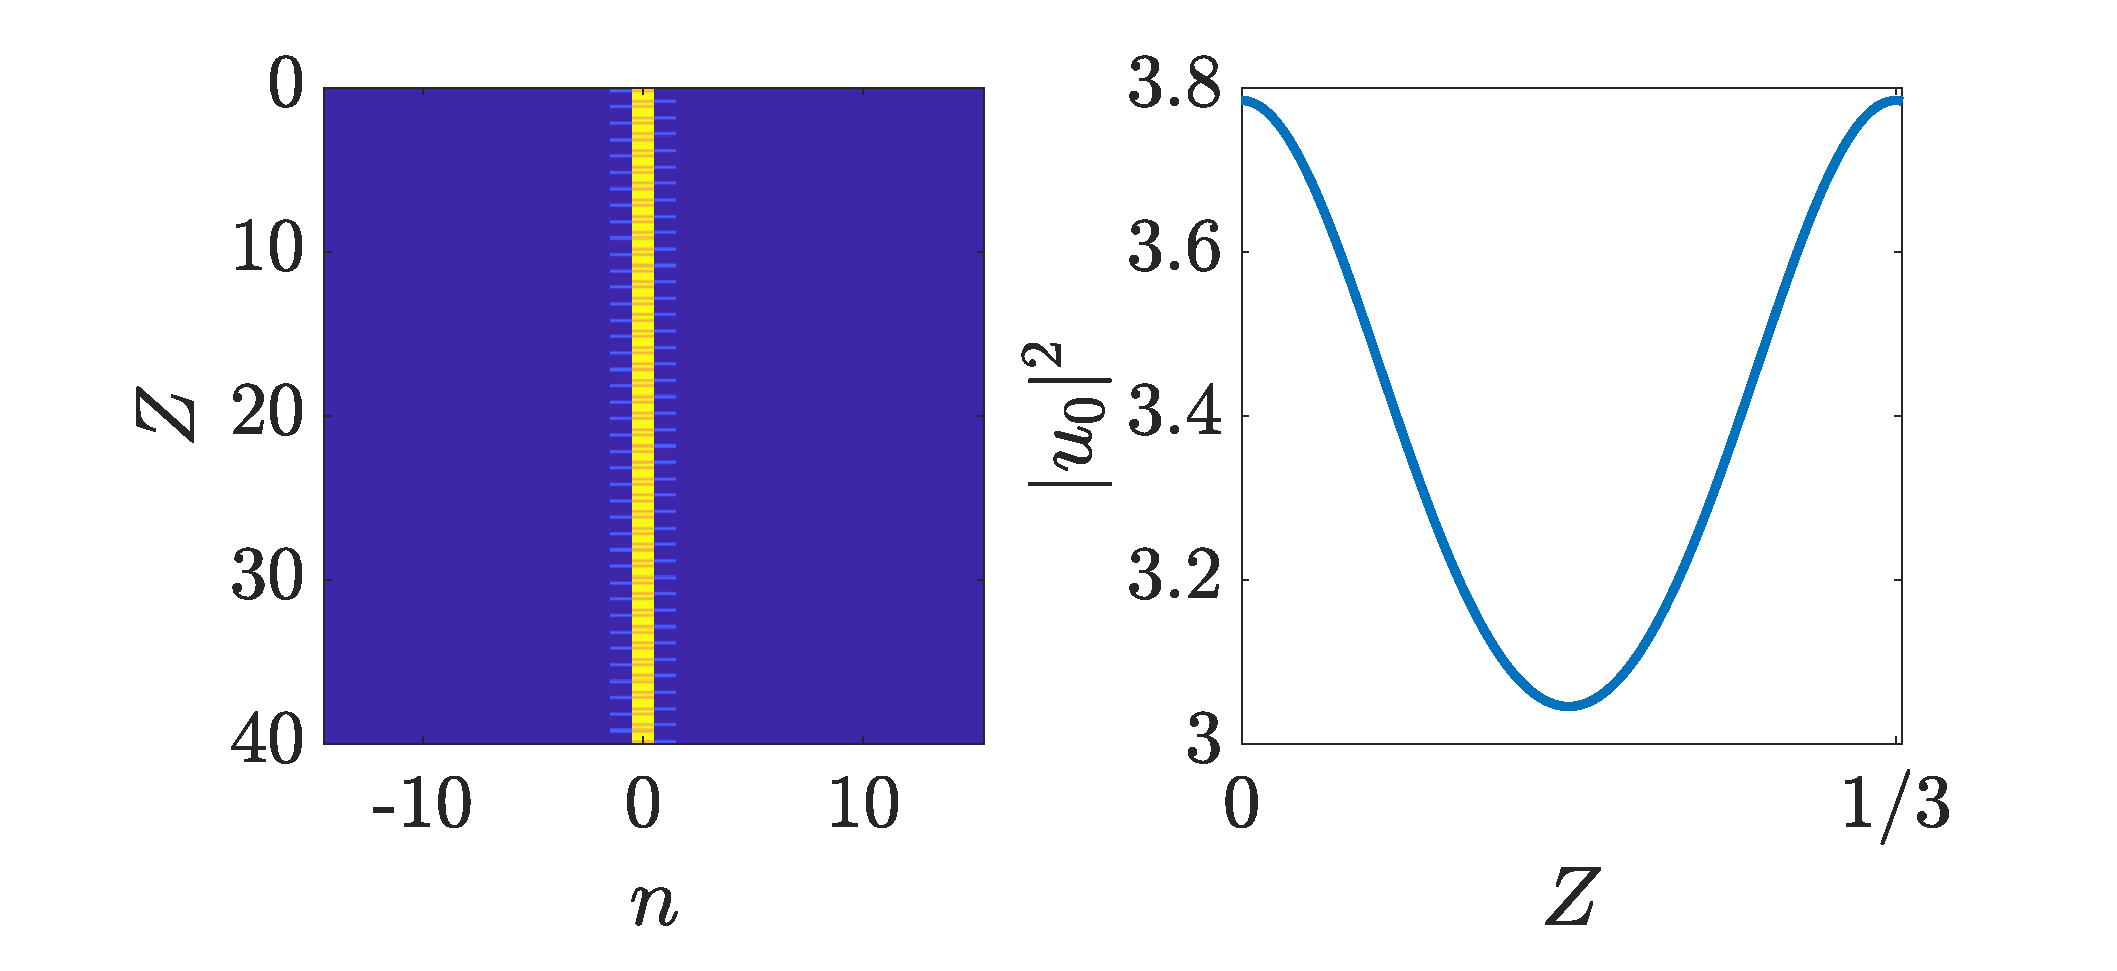
\includegraphics[width=9cm]{statsimplifiedcomplete}
    \caption{Colormap of evolution in $Z$ of single-site initial condition in simplified model (left) and power $|u_0|^2$ of site $n=0$ (right) on $Z\in[0,1/3]$ (right). Parameters chosen so that $Z_1^* = 1/3$ (top) and $Z_2^*=1/3$ (bottom).
    Starting power $P=0.0625$ (top) and $P=1.9453$ (bottom).
    $C=0.75$, $g=1$.}
    \label{fig:simplecomplete}
\end{figure}

\subsubsection{\texorpdfstring{Case 2: $P > P^*$}{Case 1: P > Pstar}}

For $P > P^*$, the solution $p(Z)$ involves the Jacobi dn function, which oscillates about 1 with period $4 K(k)/gPL$, where $K(k)$ is defined by \cref{eq:Kellipticint}. The period of oscillation becomes infinite as $P$ approaches $P^*$ from above.
As a consequence, the intensity $|u_0|^2$ exhibits small(er progressively
as $P$ is increased) amplitude oscillations with this period about the initial power $P$ (\cref{fig:simplemodel1}, right).
As in Case 1, the power initially flows to the left.
If the coupling is not cut off at $Z=1/3$ (and no other couplings are activated), there is a critical value $Z_2^*$ of $Z$ at which point the system has returned to its initial state, i.e. the powers at sites $n=0$ and $n=-1$ are once again $P$ and 0, respectively. 
For most configurations, including all of the examples in \cref{fig:simplemodel1}, $Z_2^* \neq 1/3$, thus when the coupling switches off, there has been some net transfer of power to the neighboring site $n=-1$. 
The right panel of \cref{fig:powertransfer} plots the fraction of power remaining at site $n=0$ at $Z=1/3$ for varying $C$. If this fraction is close to 1, numerical timestepping simulations show stationary solutions starting from a single-site initial condition; the closer this fraction is to 1, the longer these stationary solutions will persist before breaking up (\cref{fig:timestepsimpleabovepstar}).

As in Case 1, we note that it is possible to choose parameters so that, for the simplified model, the system returns exactly to its starting condition at $Z=1/3$, i.e. $Z_2^* = 1/3$ (\cref{fig:simplemodel1}, bottom). In this case, for a single-site initial condition with a specific starting power, the simplified model supports a localized in space, time-periodic solution which persists for a large interval in $Z$. A comparison between the evolution of the original and simplified systems is shown in the bottom panel of \cref{fig:simplecompare}. We discuss genuinely time-periodic (numerically exact) coherent structures in the full model in Subsection \cref{sec:statsol}. 
 
\begin{figure}
    \centering
    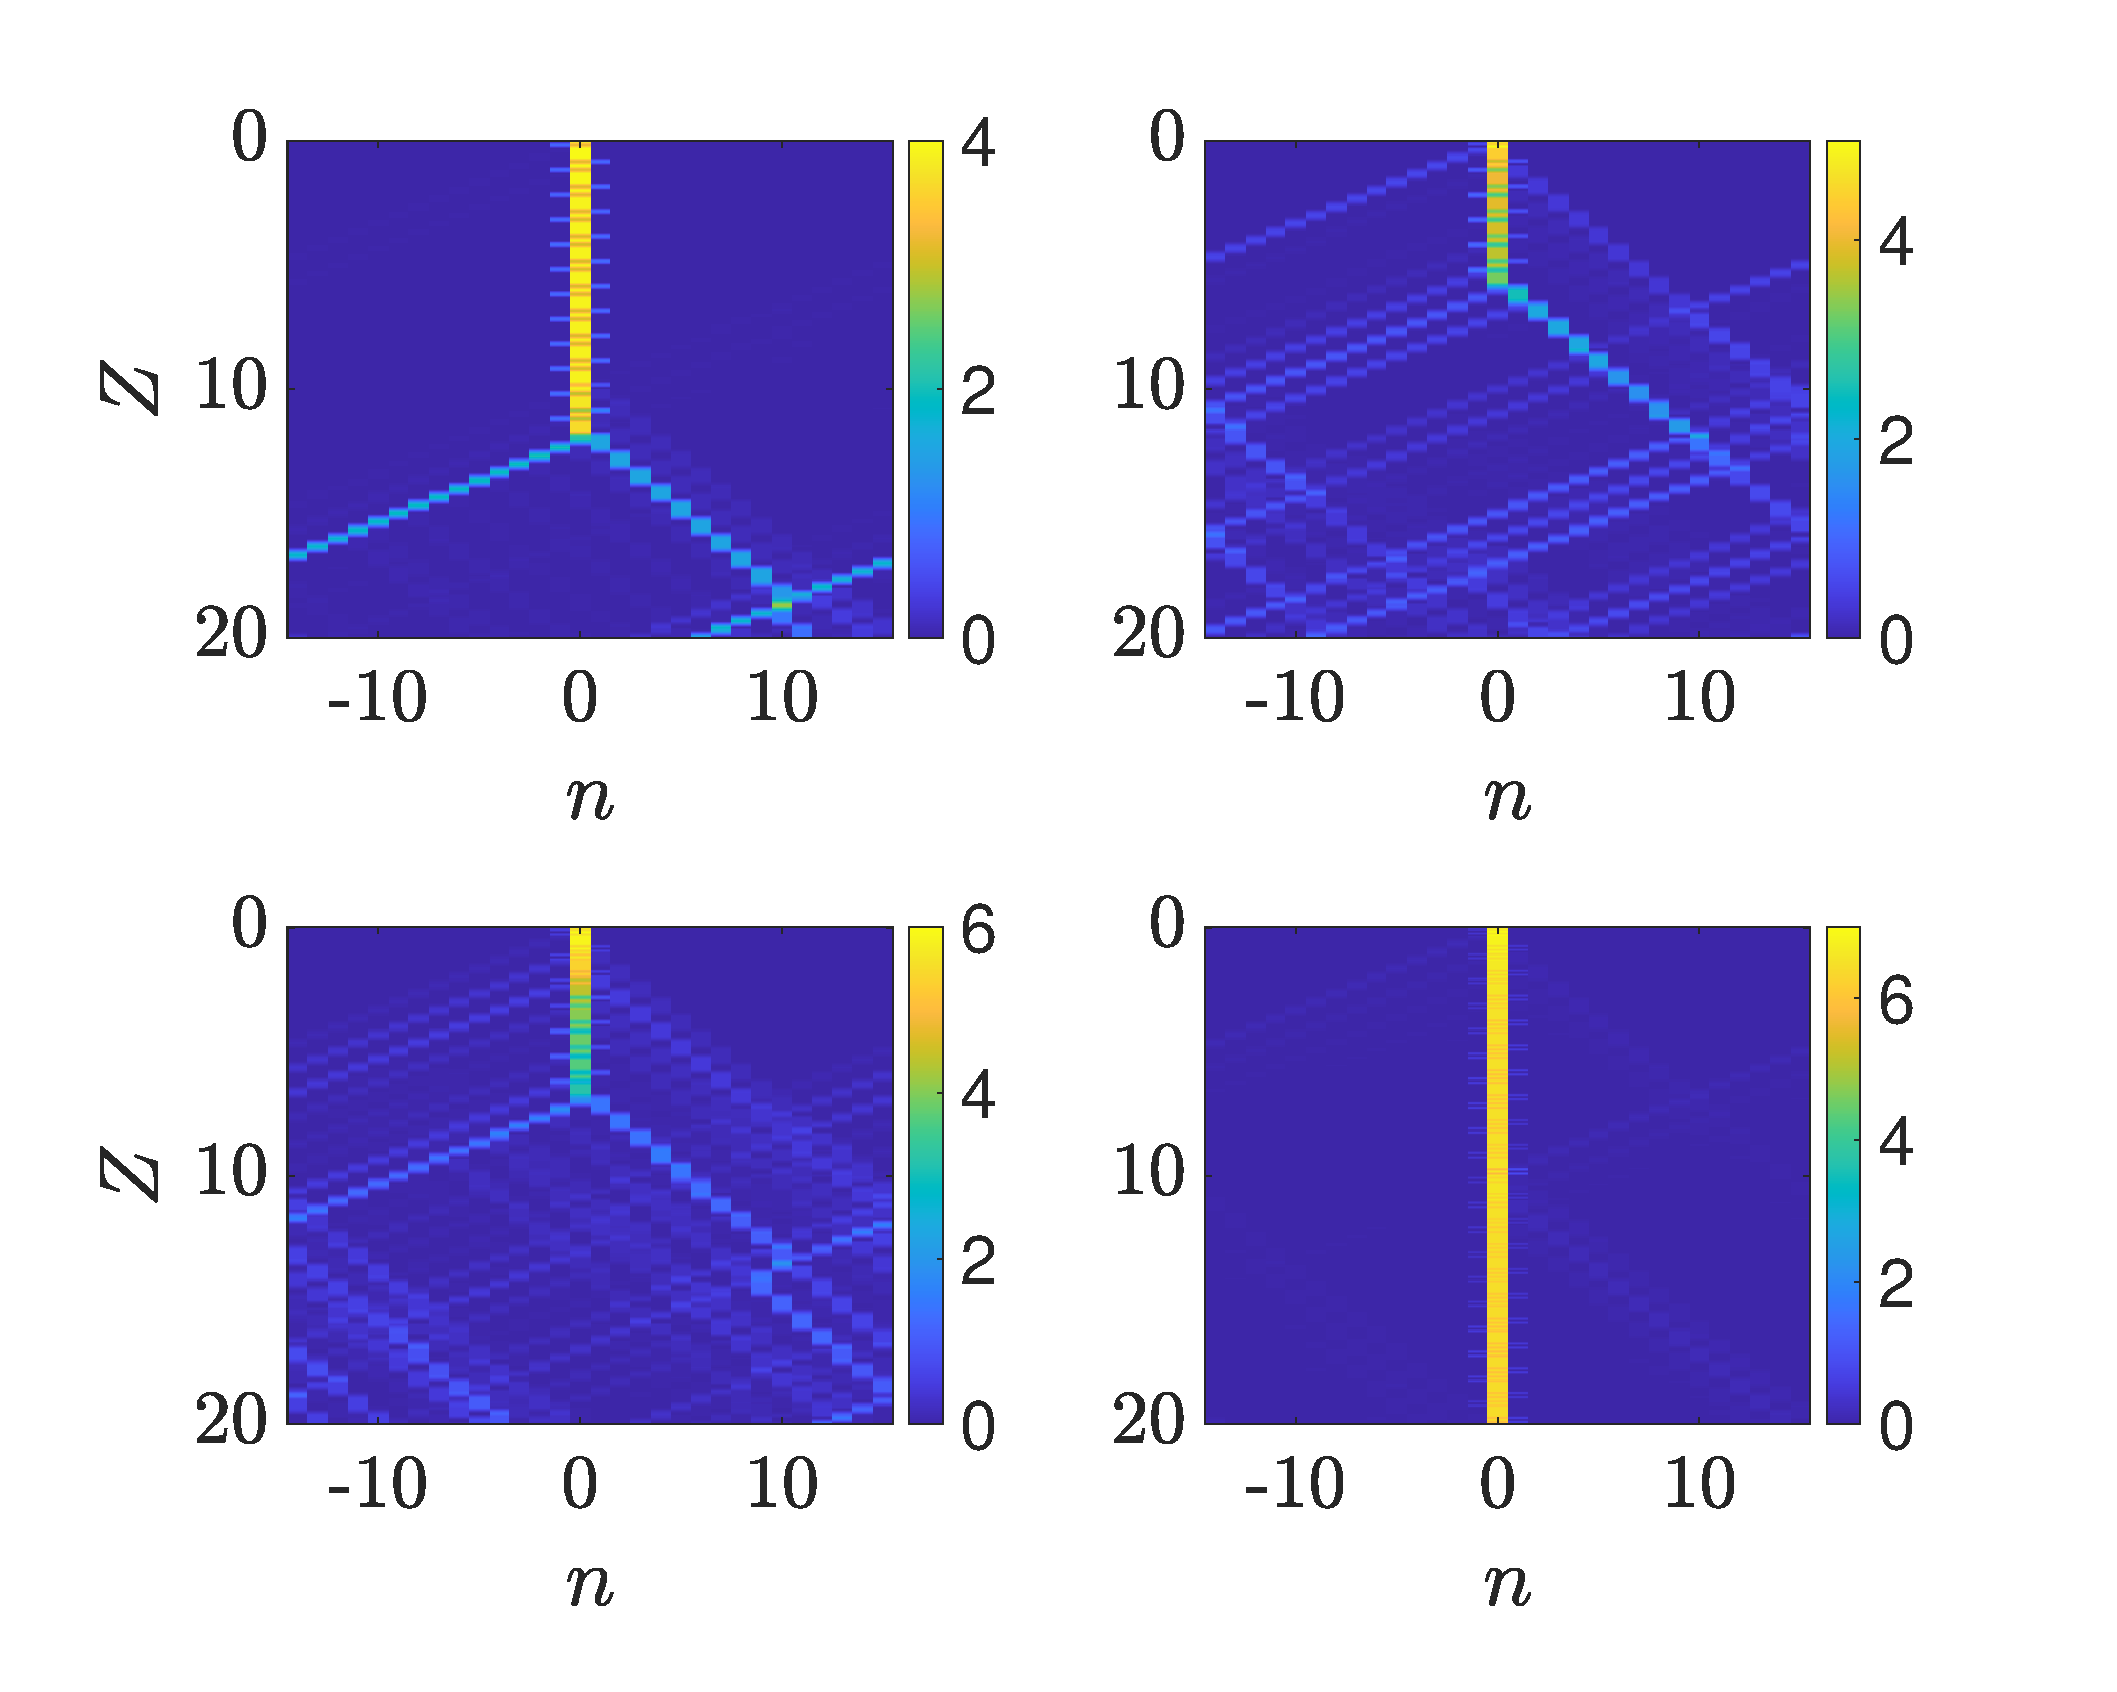
\includegraphics[width=9cm]{timestepsimpleabovepstar.eps}
    \caption{Colormap showing power of solution of equation \cref{eq:modelZ} with simplified coupling function \cref{eq:simpleJn} evolving in $Z$, starting with a single excited site at $n=0$ with power $P=4,5,6,7$, $P>P^*$ (left to right, top to bottom). Fraction of power remaining at site $n=0$ at $Z=1/3$ is 0.9938, 0.8853, 0.9815, and 0.9797 (respectively).
    $P^*=3.2$, $C=0.8$, $g=1$.}
    \label{fig:timestepsimpleabovepstar}
\end{figure}

\subsection{Coherent Structures in the Full Model}
%\subsection{Coherent structures}
\label{sec:coherent}

These evolution experiments are strongly suggestive of the fact that the system \cref{eq:modelZ} supports two classes of coherent structures: localized in space, time-periodic solutions, which are centered at a particular lattice site, and moving solutions, which reproduce themselves exactly a specific number of sites to the left or to the right. Recall that for the rescaled system \cref{eq:modelZ}, the coupling period is 1. The stationary coherent structures will be periodic orbits whose period is a multiple of the coupling period, i.e., a positive integer. We note that while it may be possible to find such solutions which have a noninteger period, Floquet analysis requires that the period of the solutions be commensurate with that of the coupling. Similarly, we will look for moving solutions that reproduce themselves, shifted left or right, after an integer period.

For appropriate choices of system parameters, we can compute both types of solutions numerically. For both localized (i.e., non-moving) and moving solutions, we use a shooting method with periodic boundary conditions imposed on $Z$, starting with a single-site initial guess. In addition, for the former 
case, we validate this method by using numerical parameter continuation with AUTO \cite{auto07p} to solve a periodic boundary value problem. Unless otherwise specified, the parameters in the section are the same as in the previous one. 

\subsubsection{Stationary (non-moving) solutions}\label{sec:statsol}

First, we look at the stationary solutions. At the anti-continuum (AC) limit ($J=0$ and $C=0$), the lattice sites are decoupled, and an initial power $P$ at lattice site $n$ will yield a standing wave solution of frequency $P$, i.e., of the form $u_n(Z) = \sqrt{P} e^{ 2 \pi i P Z}$. Since such a solution has period $1/P$, and stationary solutions must have an integer period, these solutions will exist in a discrete family for every integer period $N$, i.e. approximately $P = k/N$ for sufficiently large positive integer $k$. For period $N=1$ and the parameters in the previous section, for example, we expect to have
time-periodic, non-moving solutions for approximate integer powers $P \geq 2$. See \cref{fig:stat2} and \cref{fig:stat3} for the first two of these solutions. By looking at the intensity and the real part of the central site ($n=0$), we see that they are approximately standing waves with frequency 2 and 3 (respectively). We note that the stationary solutions do not decay to 0 with increasing $|n|$, but rather the tails exhibit small amplitude oscillatory patterns (see top right of \cref{fig:stat2} and \cref{fig:stat3}); the specific pattern of oscillations depends on the lattice size (not shown).
Looking at the sites adjacent to the central one, the left neighbor $u_{-1}$ peaks on the interval $[0,1/3]$ when the coupling $J_2(z)$ is most active, and the leftward flux at the central site is negative (indicating flow of power to the left). The right neighbor peaks on the interval $[2/3, 1]$ when the coupling $J_0(z)$ is most active and the rightward flux at the central site is negative (indicating flow of power to the right). Both leftward and rightward fluxes are close to 0 on the interval $[1/3, 2/3]$, when neither nearest-neighbor coupling is strong.

\begin{figure}
    \centering
    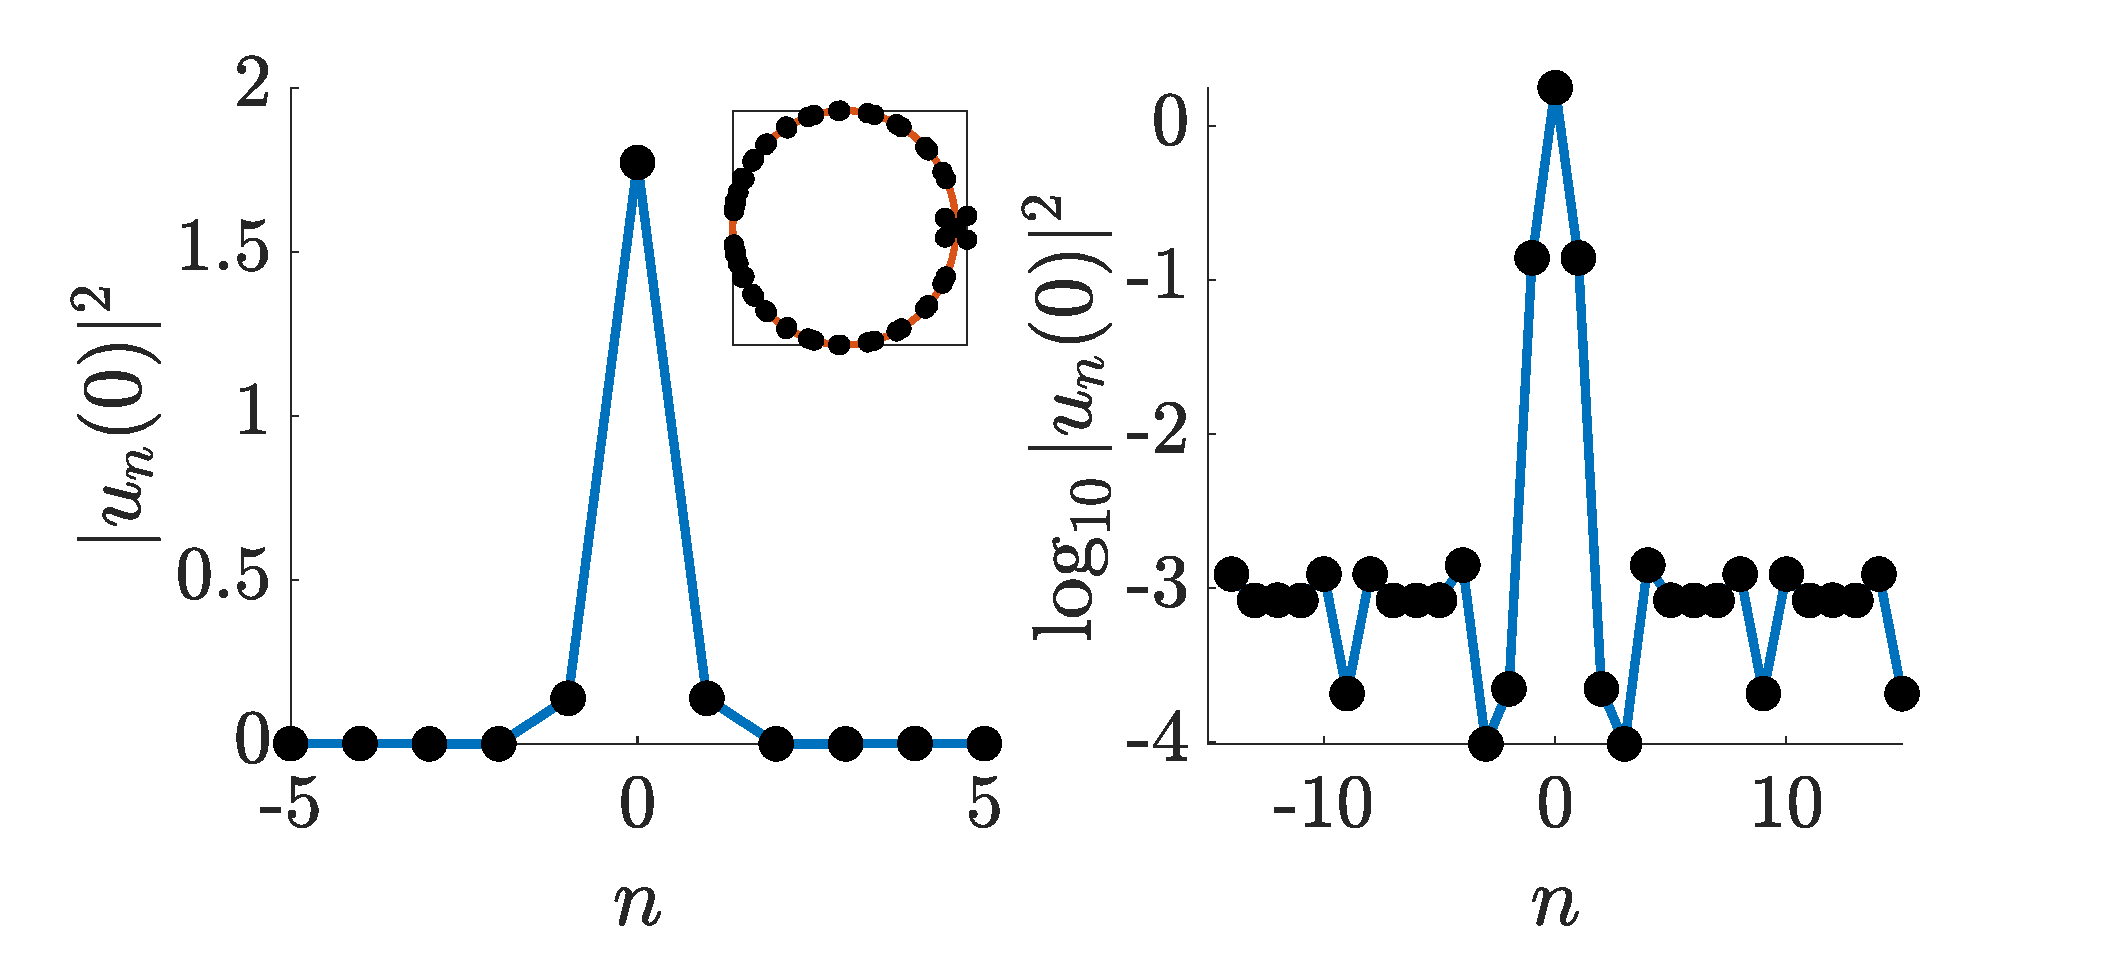
\includegraphics[width=9cm]{stat2a.eps}
    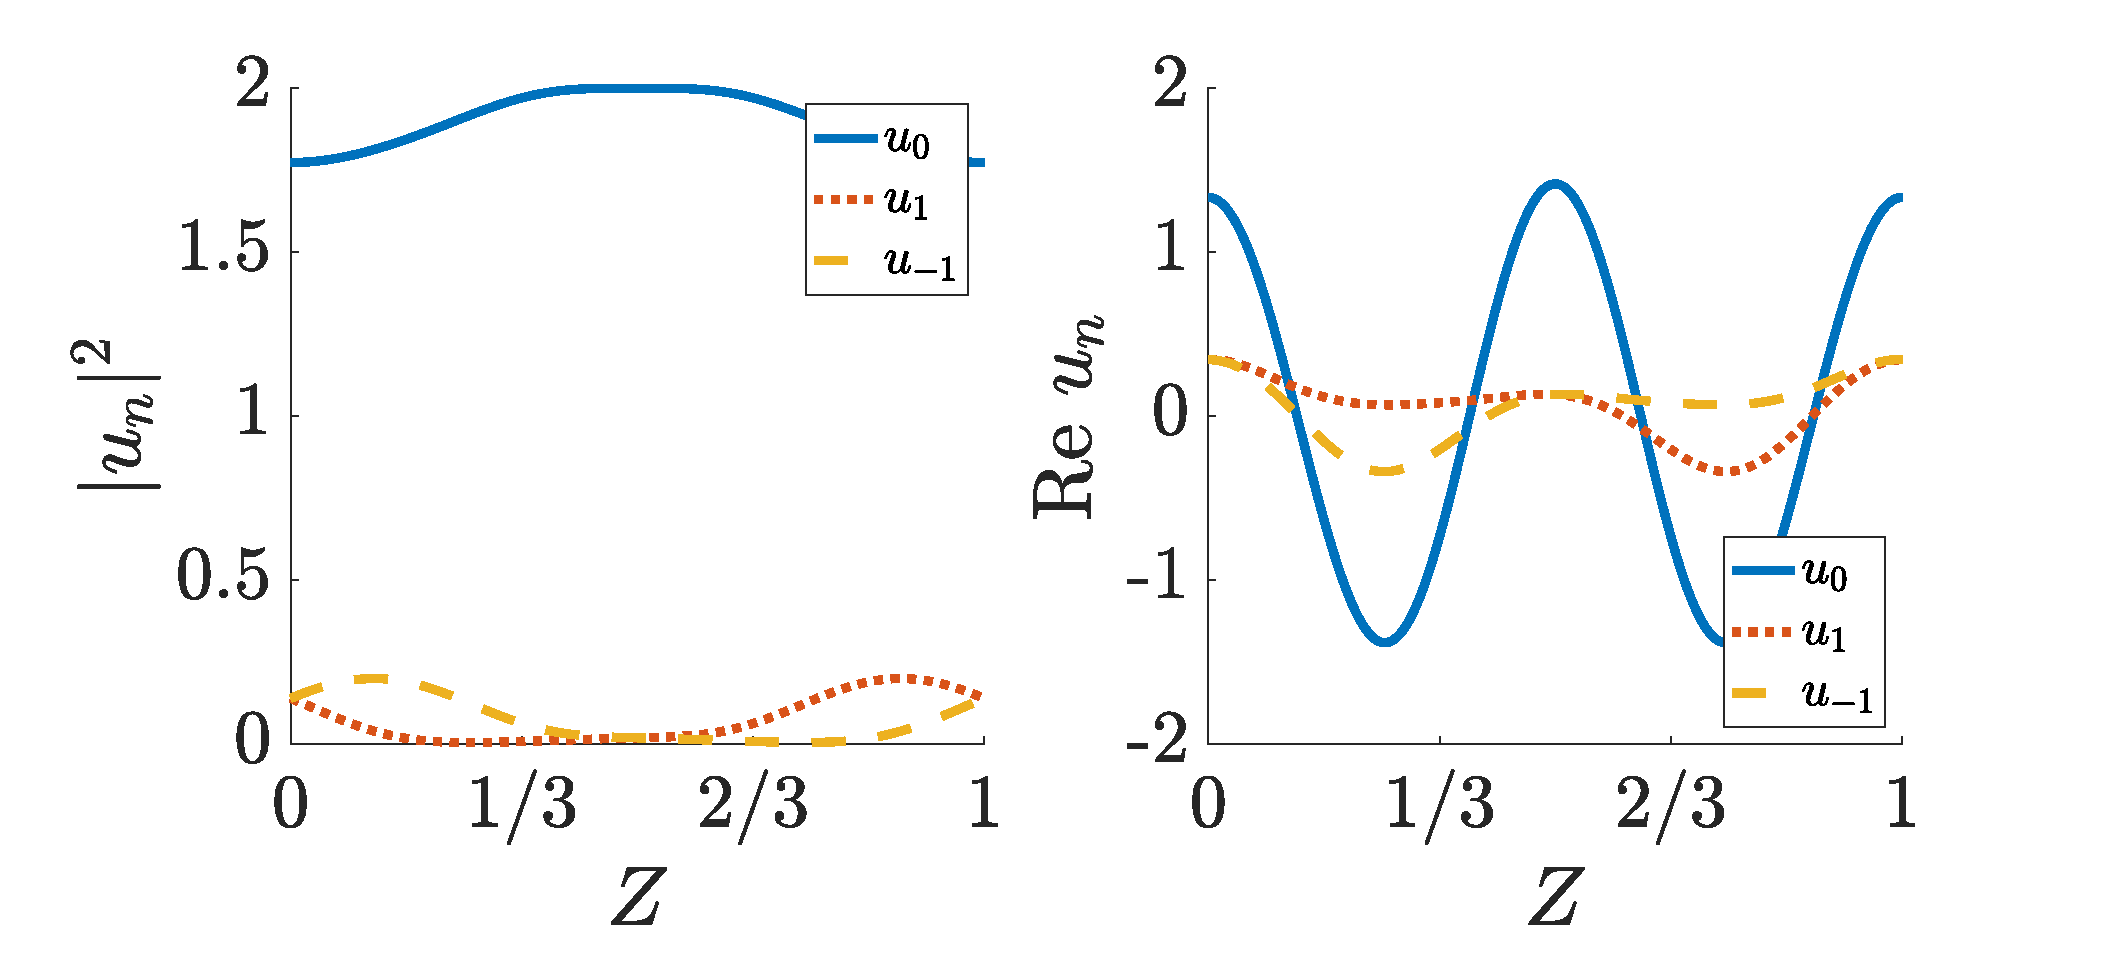
\includegraphics[width=9cm]{stat2b.eps}
    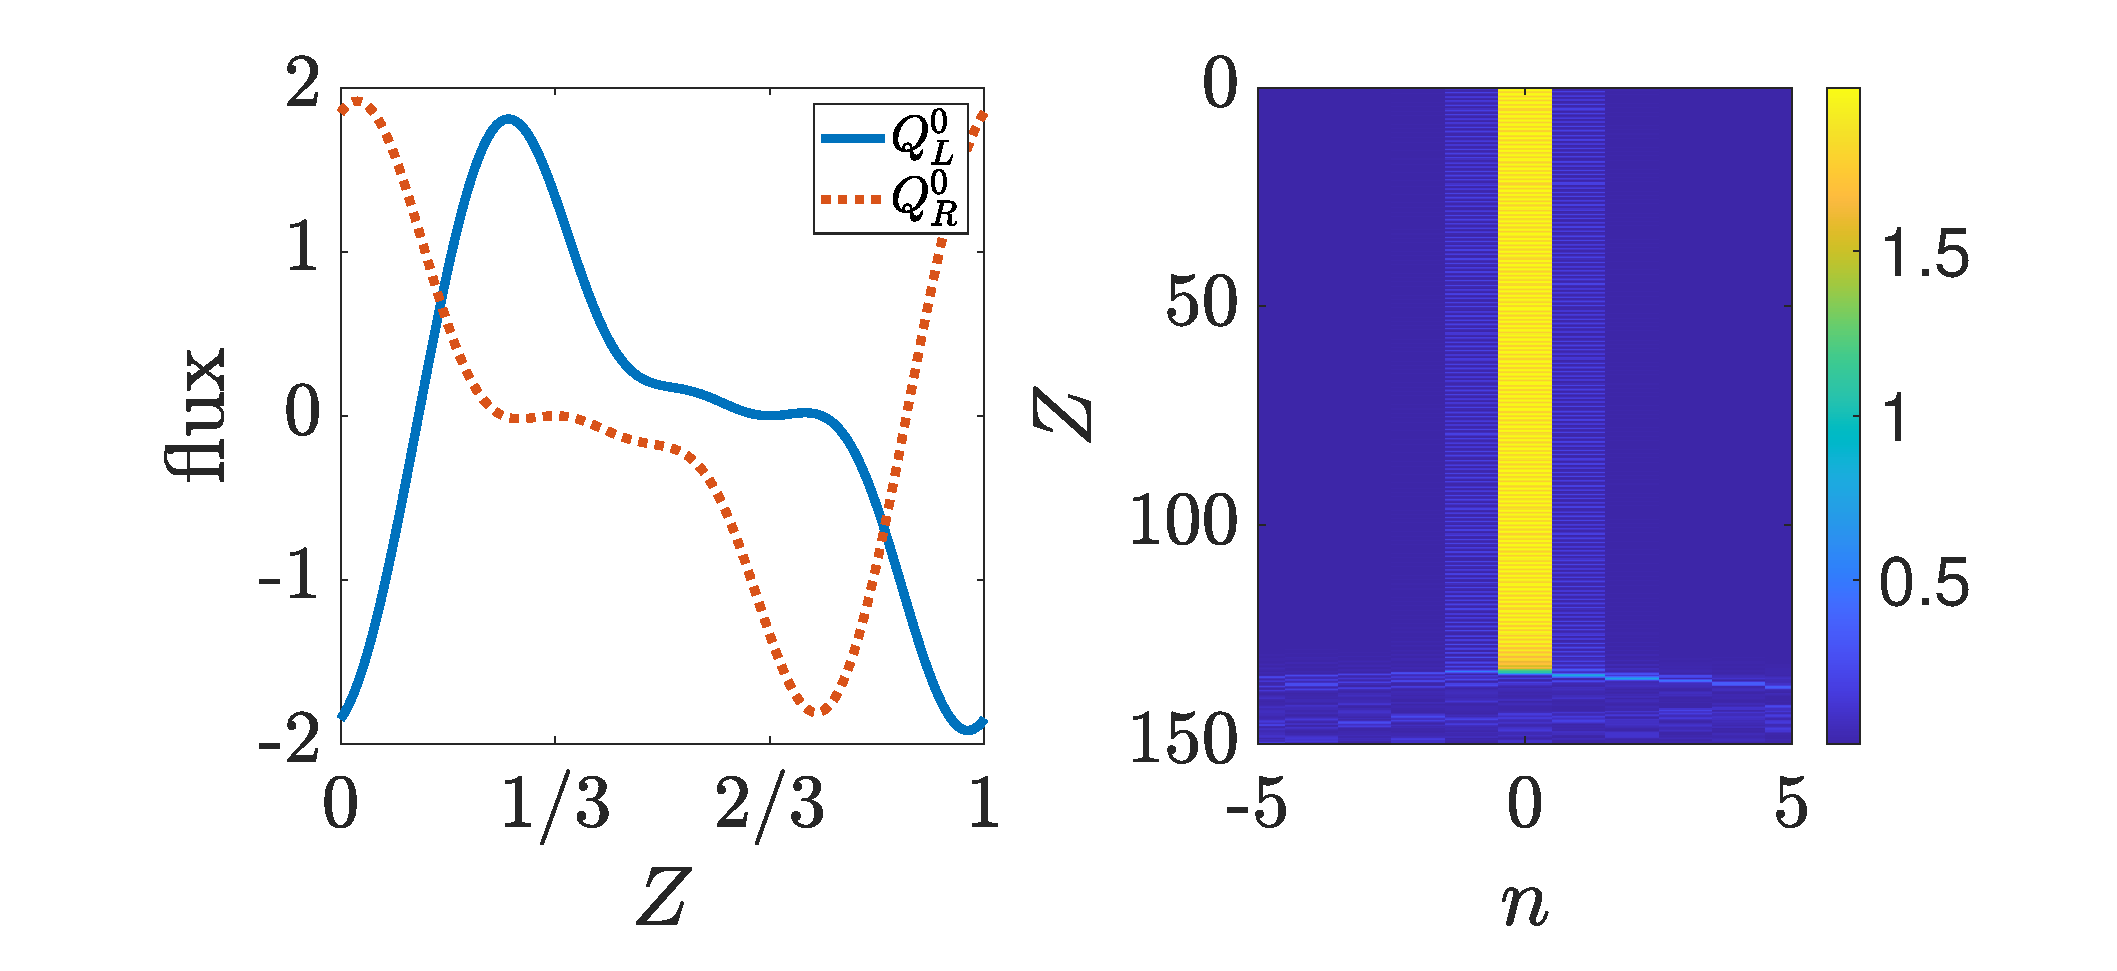
\includegraphics[width=9cm]{stat2c.eps}
    \caption{Top: initial density $|u_n(0)|^2$ (left) with inset showing Floquet multipliers, and log of initial intensity (right) for stationary solution with approximate power of 2. Middle: power (left) and real part (right) of three central sites over one period. Bottom: Left and right fluxes at central site $n=0$ (left), long term evolution in $Z$ (right). Evolution with \texttt{ode45} in Matlab with step size $10^{-2}$.} % JCM: What are the values of $C$ and $J$?}
    \label{fig:stat2}
\end{figure}

\begin{figure}
    \centering
    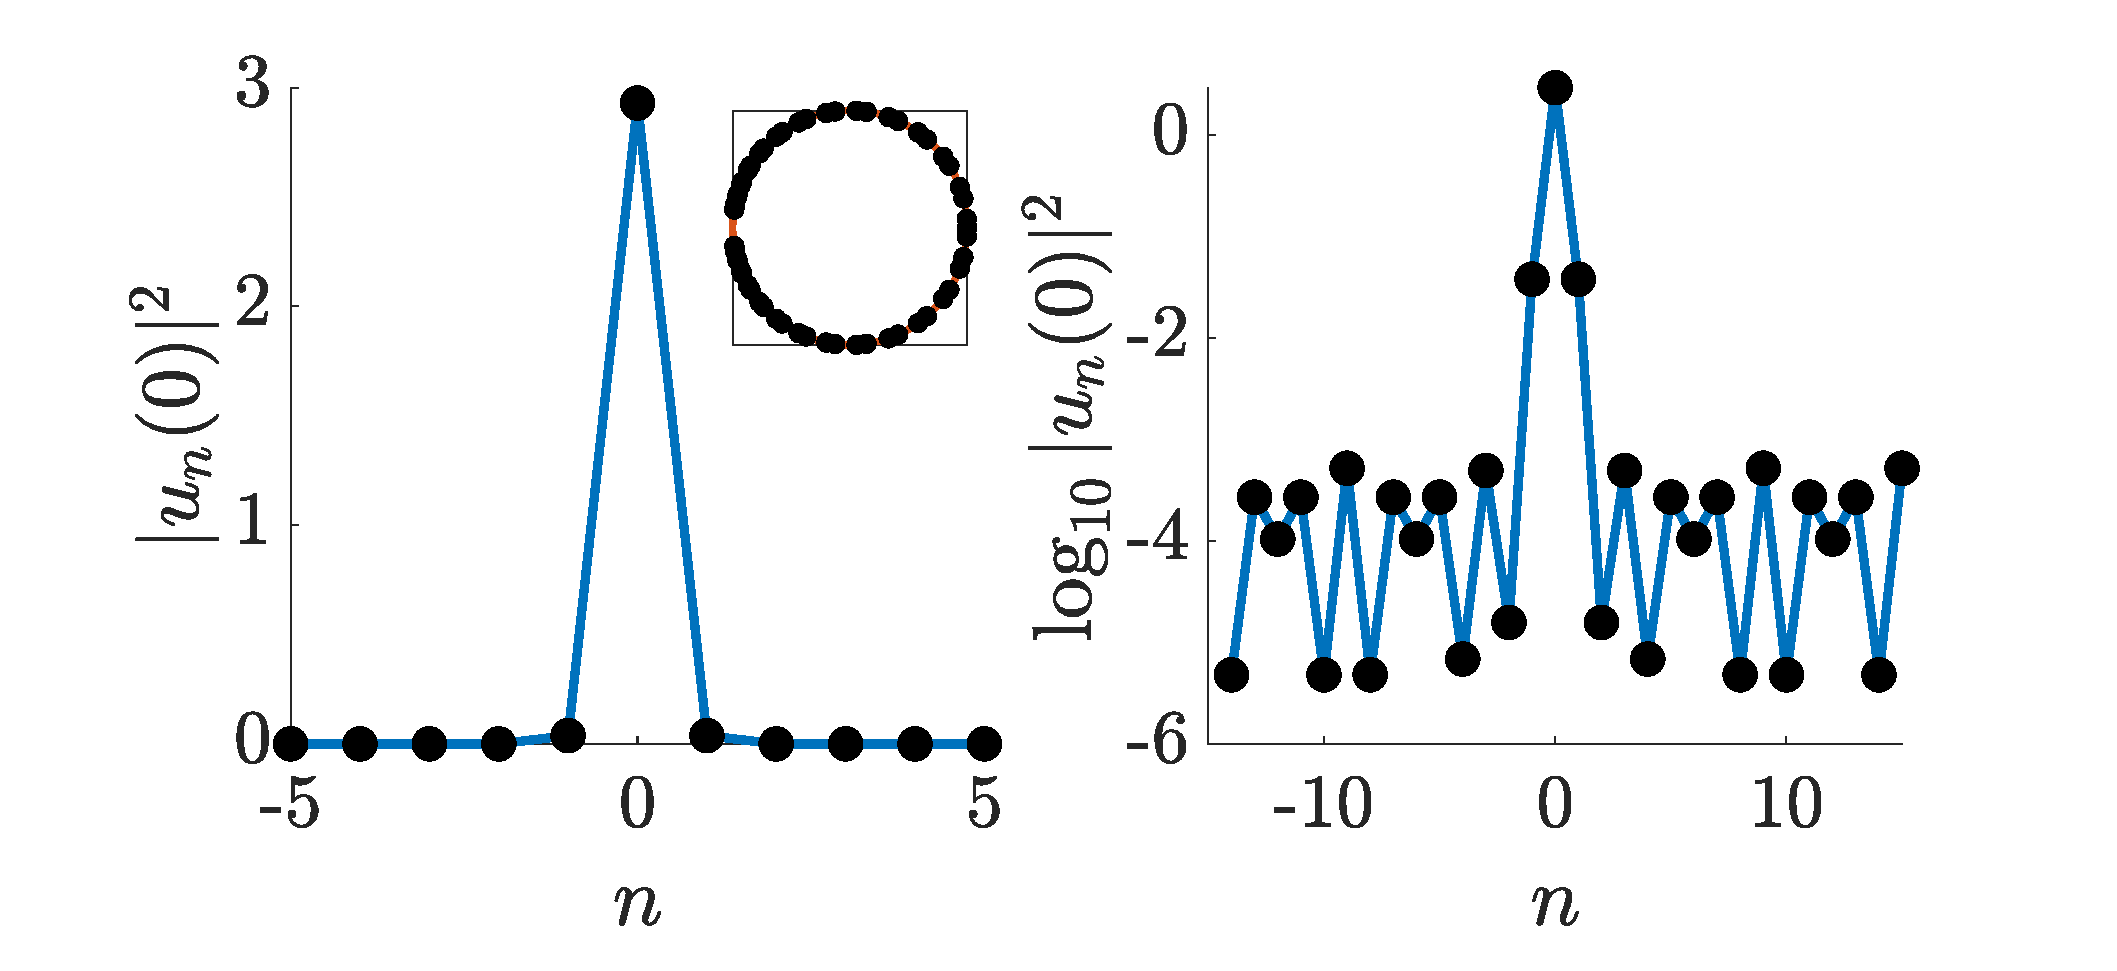
\includegraphics[width=9cm]{stat3a.eps}
    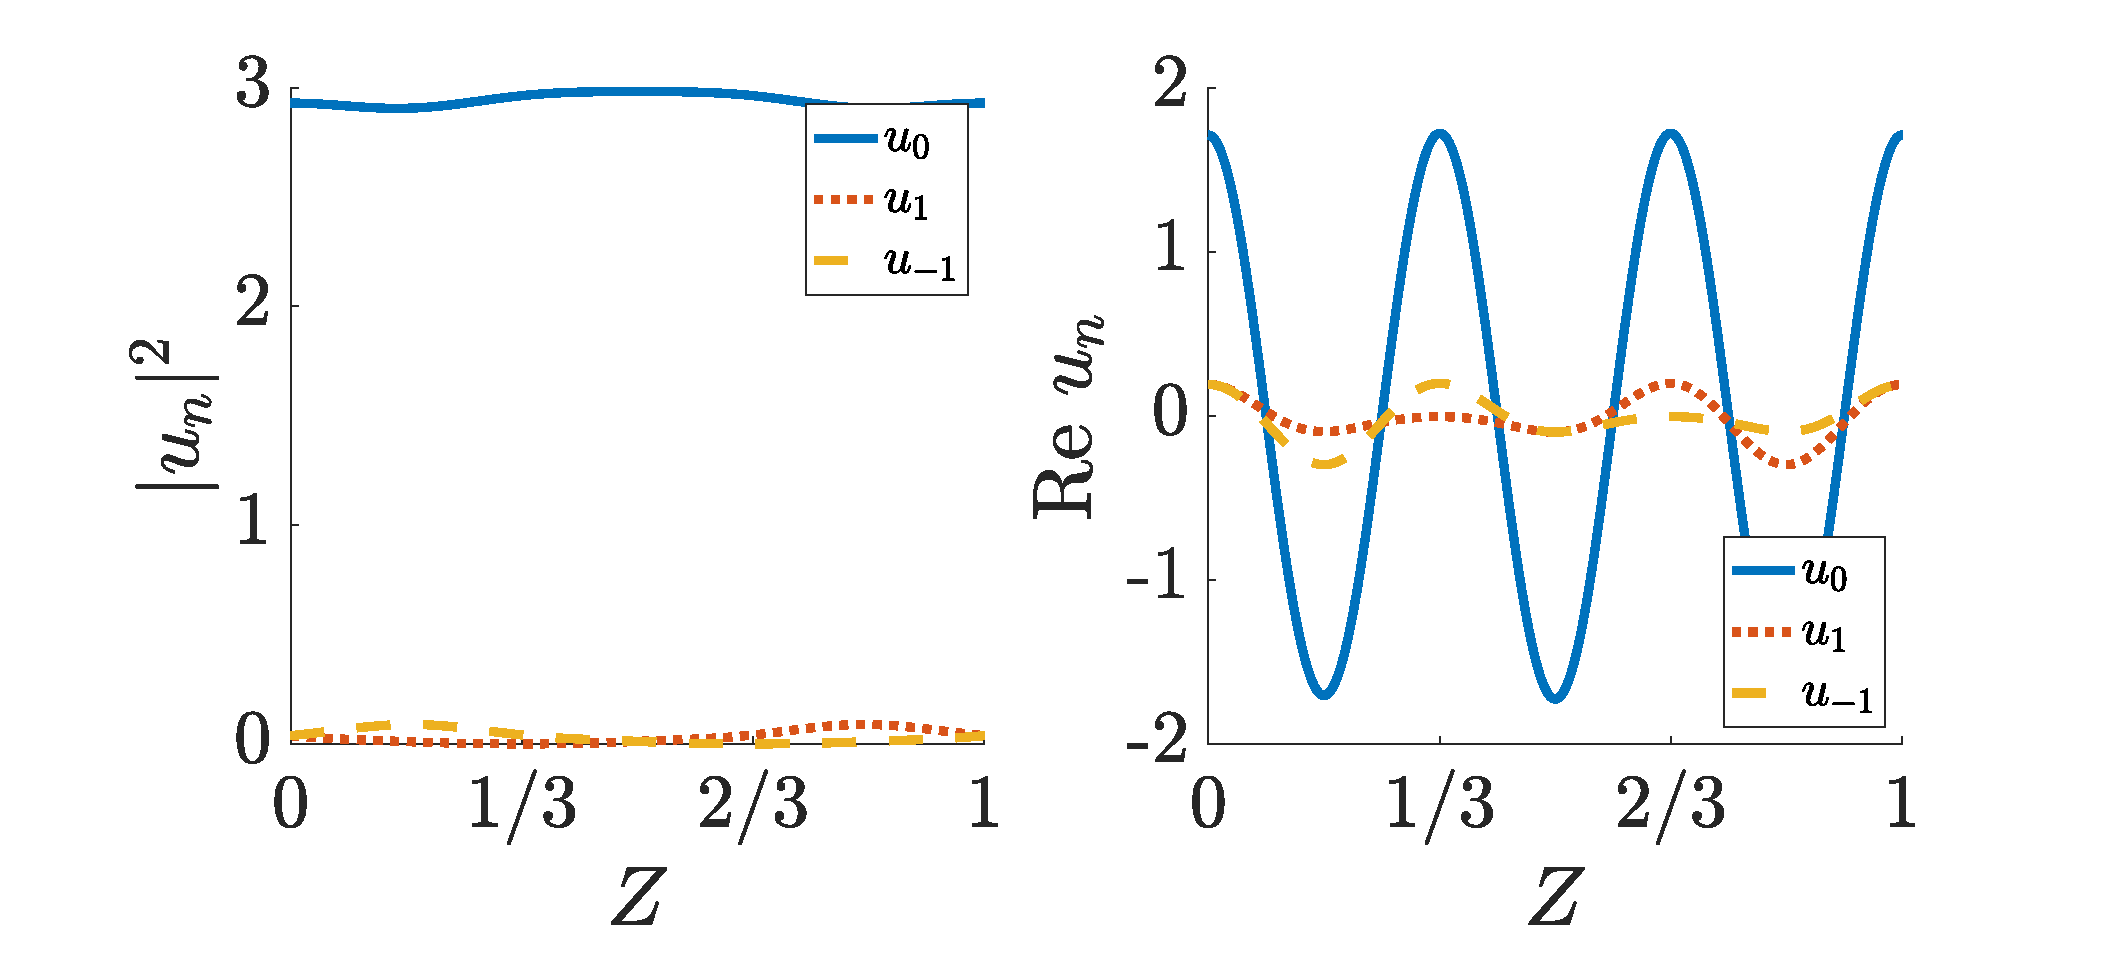
\includegraphics[width=9cm]{stat3b.eps}
    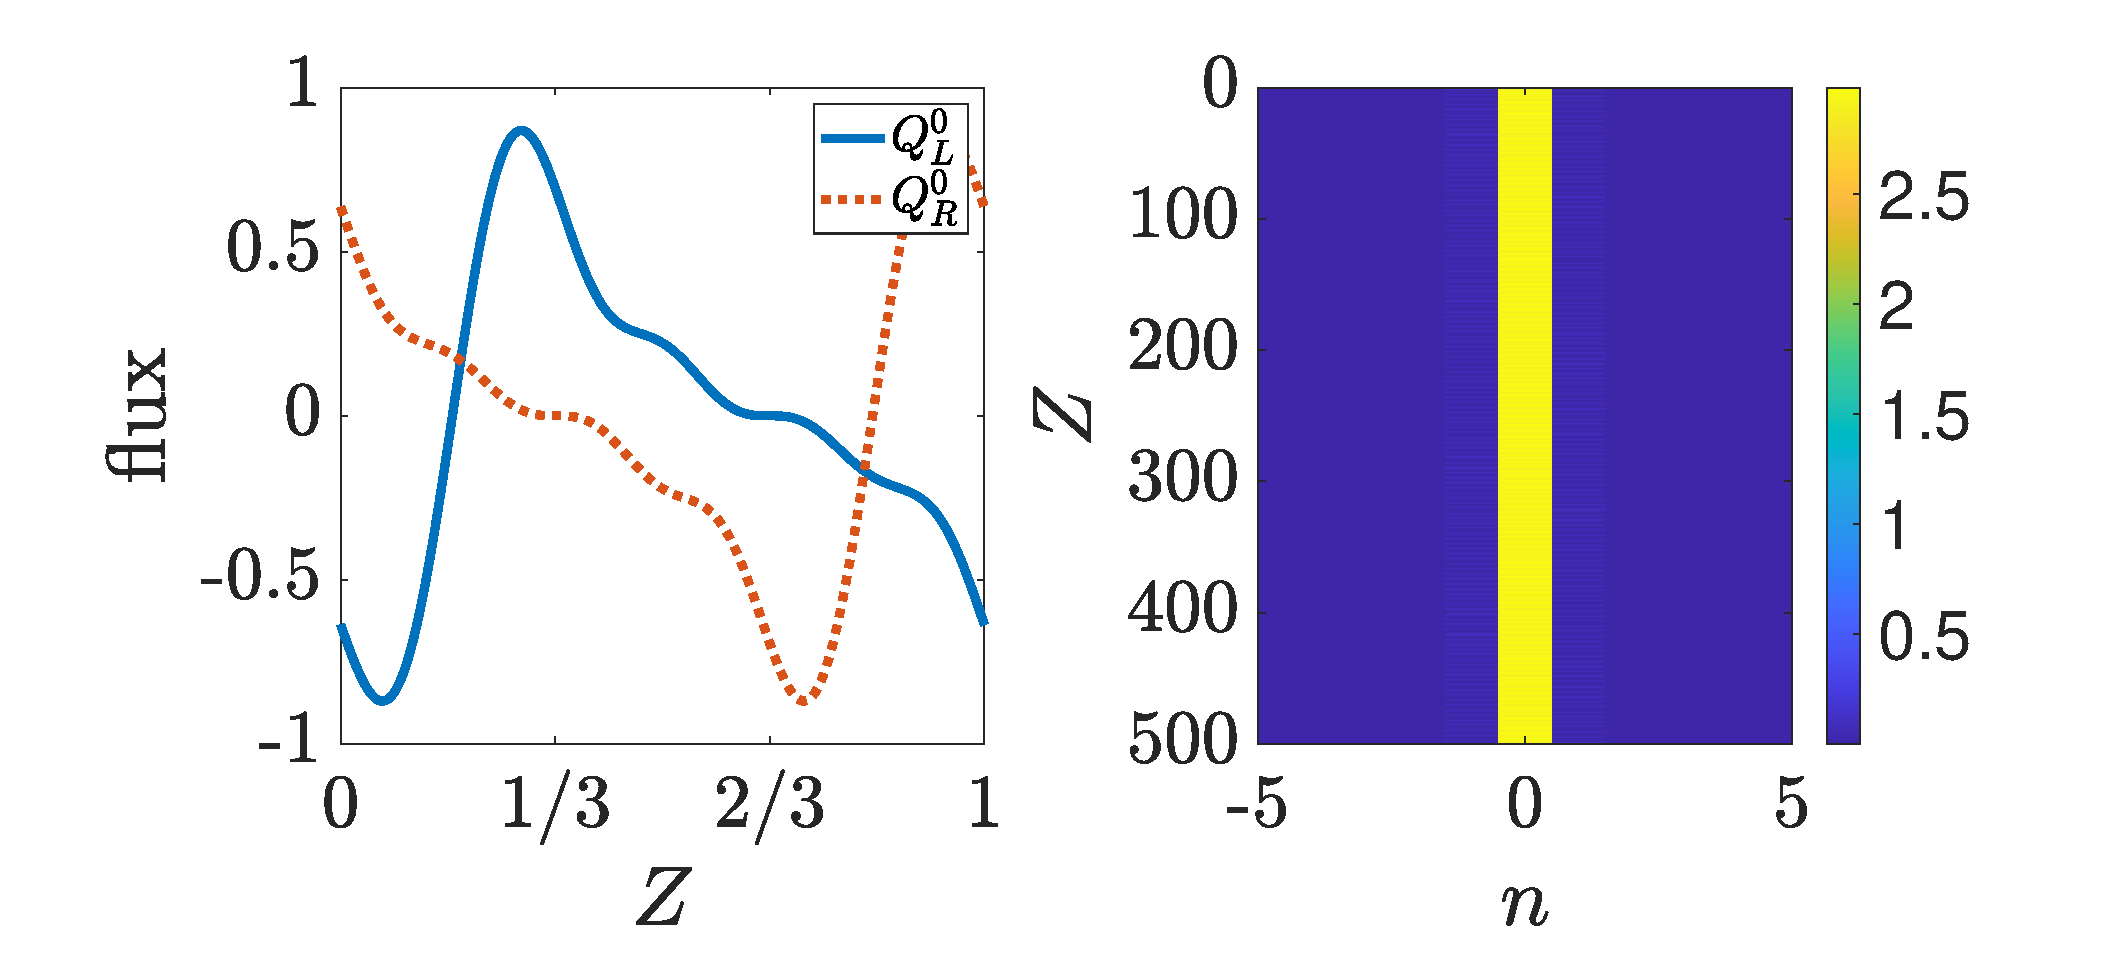
\includegraphics[width=9cm]{stat3c.eps}
    \caption{Same as \cref{fig:stat2}, but for the non-moving solution with approximate power of 3.}
    \label{fig:stat3}
\end{figure}

Since these non-mobile solutions are true periodic orbits with integer period, so that their period is equal to or commensurate with that of the coupling, their spectral stability can be determined by Floquet theory. Numerical computation of the Floquet multipliers of the stationary solutions is shown in the insets of the top left plots in \cref{fig:stat2} and \cref{fig:stat3}. The lower power solution has two pairs of Floquet multipliers off of the unit circle, which is characteristic of an oscillatory instability. Long term evolution in $Z$ (bottom right plots of \cref{fig:stat2} and \cref{fig:stat3}) shows that this solution remains coherent until approximately $Z=130$. By contrast, the Floquet spectrum of the higher power solution lies on the unit circle, indicating spectral stability. Long term evolution in $Z$ shows that this solution is still coherent at $Z=500$.

Using parameter continuation, we start with the DNLS soliton at $C=0$ and slowly vary $C$, tracing the curves in \cref{fig:statAC} ($J_0 = 0.05$ throughout). Since we are looking for solutions with period 1, the starting power must take integer values so that the frequency of the DNLS standing wave at $C=0$ is commensurate with this period. In all cases, a turning point is reached, as $C$ is increased, at which point the parameter continuation in the
coupling parameter $C$ reverses direction. This turning point occurs at a larger value of $C$ for solutions which start at a higher power at $C=0$. All stationary solutions initially have their Floquet spectrum confined to the unit circle, thus are spectrally stable. Spectral stability is lost at some point before the turning point observed in the graph, when Floquet multipliers collide and leave the unit circle, creating an oscillatory instability. Solutions on the upper branches of the bifurcation diagram are periodic solutions to the DNLS which are not pure standing waves. To leading order, these upper solutions are the sum of two Fourier modes, % JCM: only two?
as opposed to standing waves, which are a single Fourier mode. Substituting the finite Fourier ansatz 
\[
u_n(Z) = \sum_{k=-N}^N a_{n,k} e^{2 \pi i k z}
\]
into \cref{eq:modelZ} and projecting onto each of the Fourier basis functions, we can obtain expressions for the coefficients $a_{n,k}$ for each wavenumber $k$. An FFT of the numerical solution on the upper branches suggests that the solutions at each site are composed predominantly of the modes with wavenumbers 0 and 1. Thus, to leading order, these solutions are of the form $u_n(Z) = a_{n,0} + a_{n,1} e^{2 \pi i \omega Z}$, where the coefficients $a_{n,0}$ and $a_{n,1}$ satisfy 
\begin{align*}
&J_0(a_{n+1,0}+a_{n-1,0}) + a_{n,0}^3 + 2 a_{n,1}^2 a_{n,0} = 0 \\
&J_0(a_{n+1,1}+a_{n-1,1}) + a_{n,1}^3 - w a_{n,1} + 2 a_{n,1} a_{n,0}^2 = 0.
\end{align*}
We note that if $a_{n,0} = 0$ for all $n$, the second equation reduces to DNLS, in which case the solution is a standing wave.

\begin{figure}
    \centering
    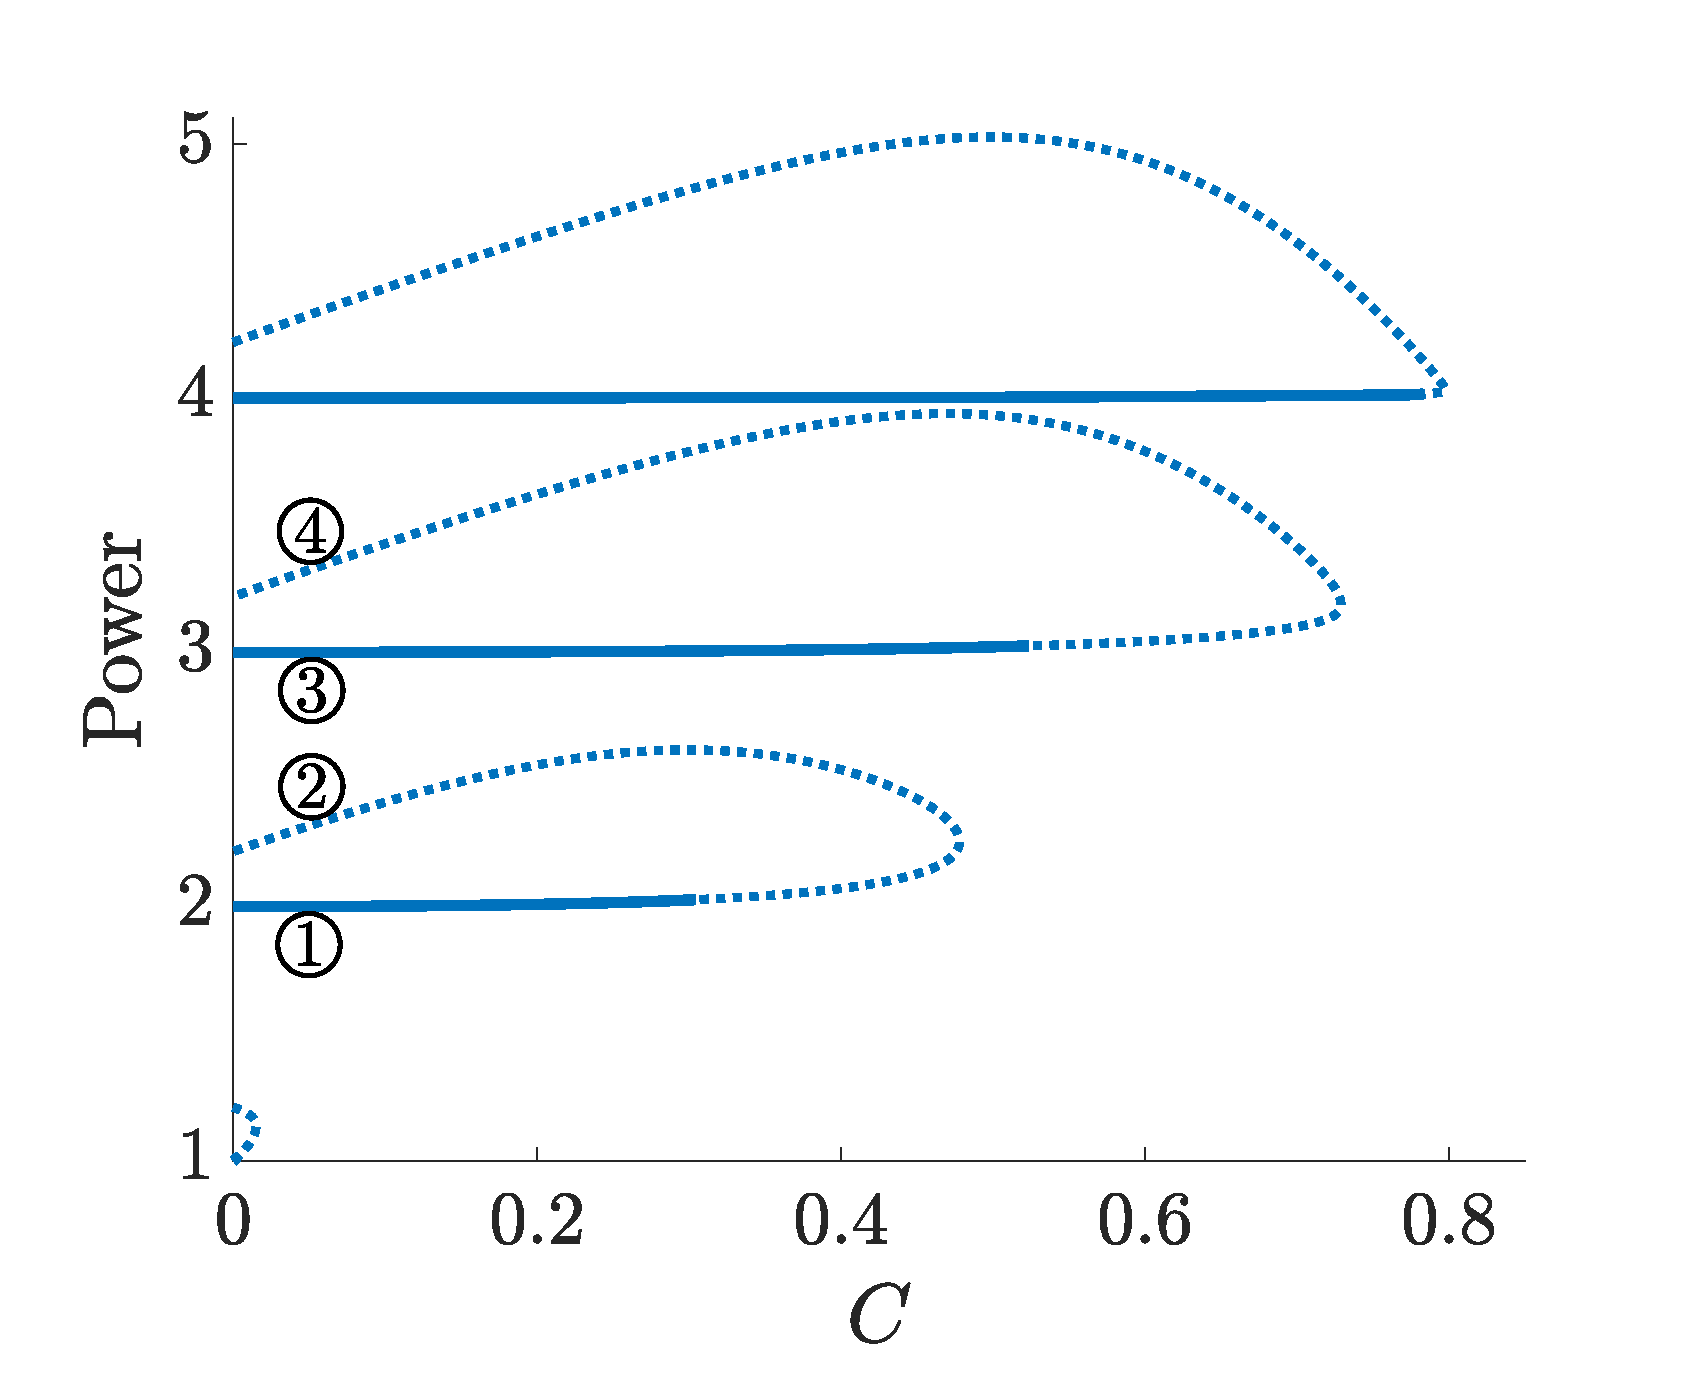
\includegraphics[width=8cm]{stat1234AC.eps}
    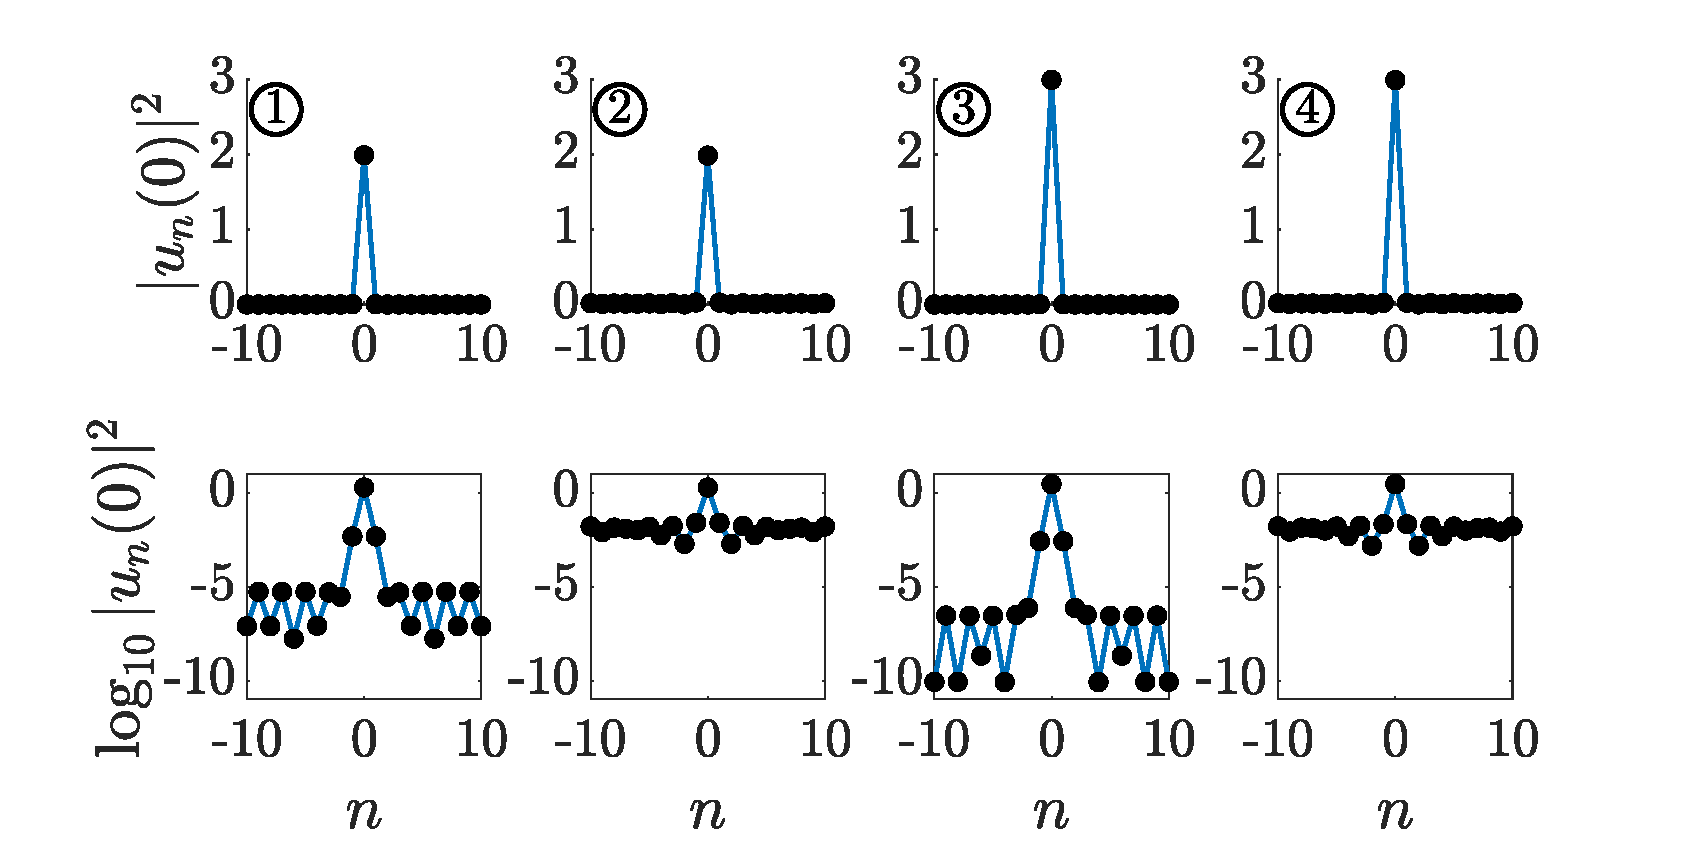
\includegraphics[width=8cm]{stat1234ACsols.eps}
    \caption{Branches of stationary solutions with period (in $Z$) of 1, obtained from numerical parameter continuation starting with DNLS soliton at $C=0$. Bottom plots show power (top) and log power (bottom) of initial condition, correspond to $C=0.05$ at labeled points on bifurcation diagram. Solid lines correspond to solutions with Floquet spectrum contained in unit circle, dotted lines correspond to solution with some Floquet spectrum outside of unit circle. Solutions on other branches at these values of $C$ are qualitatively similar.} % JCM: can be done a similar plot using the approach of Section IV?
    \label{fig:statAC}
\end{figure}

We can also continue solutions in the coupling period $L$ (\cref{fig:statcontL}). The intensity of the central peak decreases with increasing $L$, thus solutions with greater starting power at $L=2\pi$ persist for higher $L$. Again, there is a turning point where the continuation reverses directions, which occurs at larger $L$ for higher power branches. The central site for the upper and lower branches of each loop has approximately the same intensity; the higher power of the upper branches is due to larger intensity in the tails of the solutions. For contrast, the spatial period of the solutions in \cite[Figure 2]{Jurgensen2021} is $L=8000$; we would have to start with a solution with extremely high power at $L=2\pi$ to be able to reach such a large $L$.

\begin{figure}
    \centering
    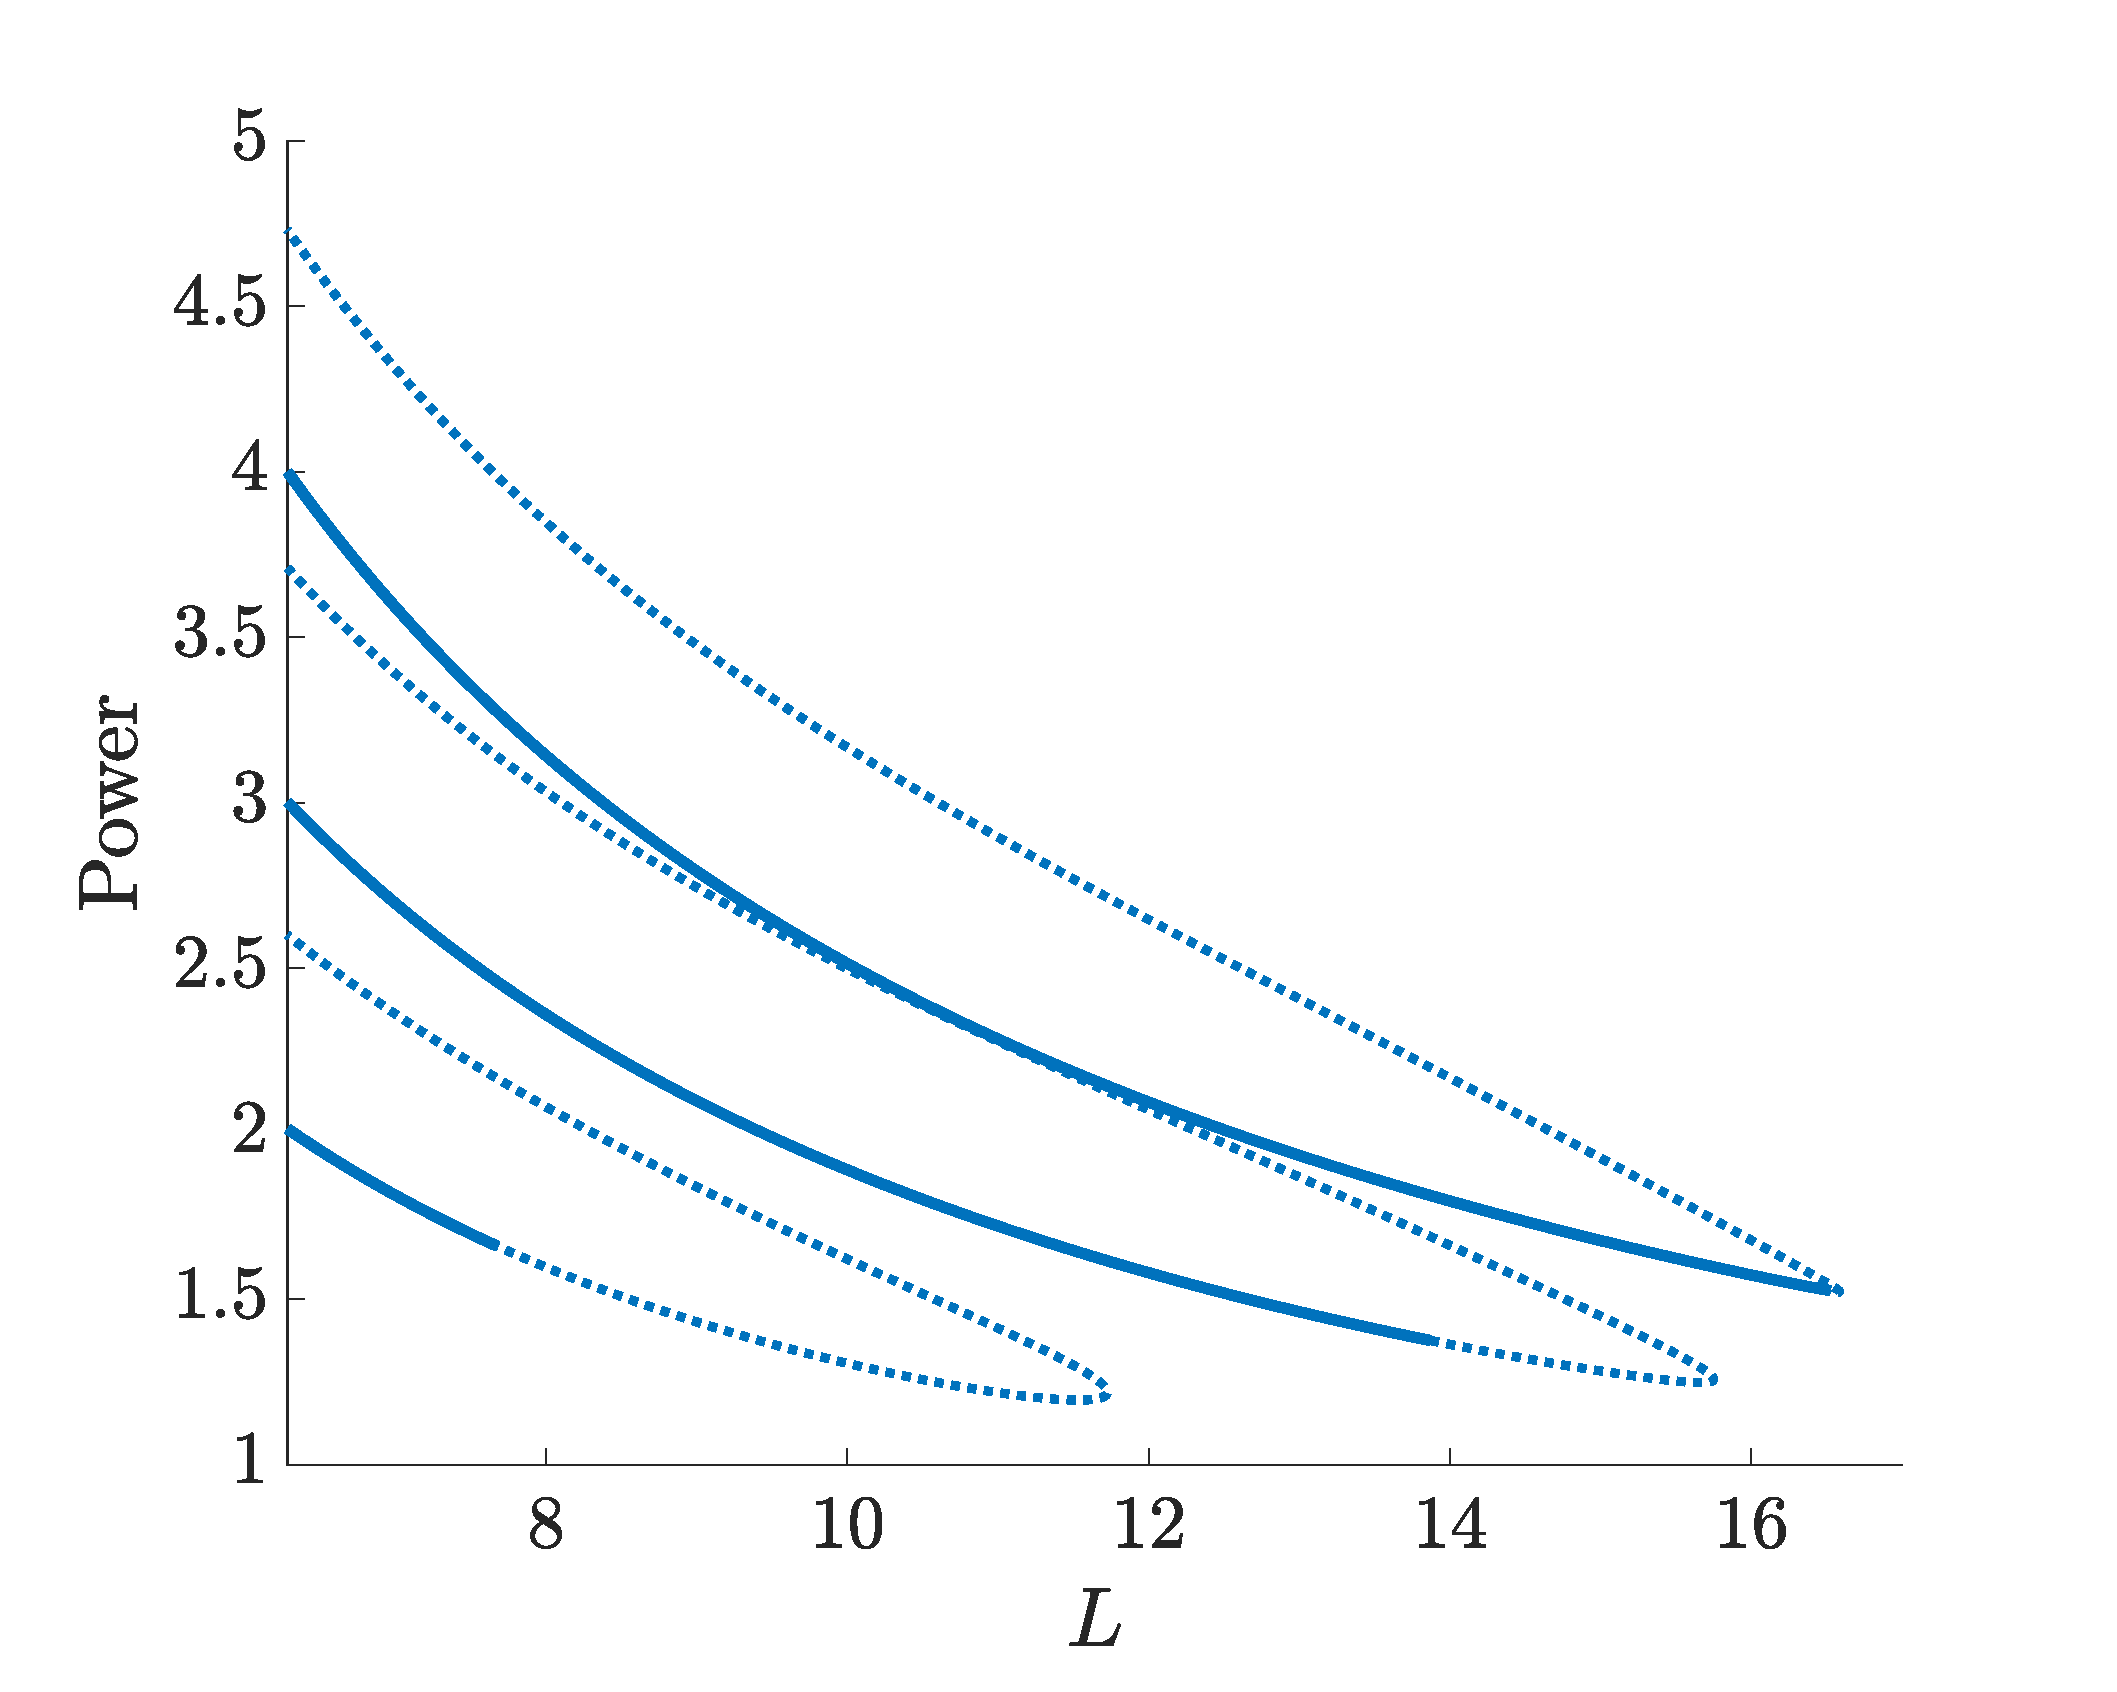
\includegraphics[width=8cm]{stat234contL.eps}
    \caption{Power vs. coupling period $L$ for solutions with approximate power of 2, and 4 at $L = 2\pi$. Solid lines correspond to solutions with Floquet spectrum contained in unit circle, dotted lines correspond to solution with some Floquet spectrum outside of unit circle. Diagram is only shown for $L\geq 2\pi$. Parameters $J_0 = 0.05$ and $C=0.25$.}
    \label{fig:statcontL}
\end{figure}

Finally, we note that, while we have only considered non-moving solutions with period of 1, stationary solutions do exist for other positive integer periods. For example, if we start with a single-site initial condition with power $k/2$ for positive, odd integer $k$, we expect that we will obtain a stationary solution with period 2. (We have verified that this is the case for single-site initial conditions with power 3/2 and 5/2). While, in principle, this can be done for any integer period, it becomes computationally intractable for larger periods.

\subsubsection{Moving solutions}\label{sec:movingsol}

Next, we look for moving solutions. For a given lattice size $m$, we find that leftward moving solutions exist (\cref{fig:leftsol}) for all values of $C$ within an interval $[C_L(m), C_R(m)]$ (see top right and bottom left of \cref{fig:leftdiag}).
These are true coherent structures, in that the entire solution reproduces itself exactly after one period, shifted three sites to the left. (In the numerical simulation, where we are using periodic boundary conditions on the lattice, we can think of this as a ``circular shift''). Generically, these solutions have oscillatory tails (\cref{fig:leftsol}, top right), and the amplitude of these oscillations depends on the lattice size (\cref{fig:leftdiag}, top left). 
Notice, however, that the corresponding wavenumber in the far field does not.
At a critical value $C^*$ of $C$ ($C^* = 0.4709$ for $J_0 = 0.05$ and $L=2\pi$), the tail oscillations vanish, leaving a localized traveling solution (\cref{fig:leftdiag}, bottom right). Most notably, the value of $C^*$ is independent of the lattice size $m$, although it does depend on both $L$ and $J_0$ (\cref{fig:Cstar}). The left moving solution appears to be stable when $C=C^*$ (see \cref{fig:movelong}, left); at minimum, it persists unchanged for at least 1000 periods. In addition, the solution appears to be stable for an interval in $C$ containing $C^*$ (not shown). 
The presence of $C^*$ seems to suggest an analogy with the so-called Stokes
constant calculation in similar such traveling (DNLS-type) problems as in the
work of~\cite{igorb}. Further expanding on this connection could be an 
interesting problem for future (but is outside the scope of the present work).
Since the traveling solution is not a periodic orbit, we cannot use Floquet analysis to determine its spectral stability. % JCM: is this sentence hanging?
We note that while the parameter continuation in the bottom left of \cref{fig:leftdiag} continues past the turning points at $C_L(m)$ and $C_R(m)$, this merely represents growth of the tail oscillations, while the power of the central site remains essentially unchanged; since none of these solutions are stable, the continuation diagram is not shown past these turning points. % JCM: I wonder why there are no vanish of the tails

Similar results are obtained for the right-moving solutions (\cref{fig:rightsol} and \cref{fig:rightdiag}). Once again, the tail oscillations vanish at a critical value $C^*$ of $C$ ($C^* = 0.5054$ for $J_0 = 0.05$ and $L=2\pi$), which is close, but not equal to, the value for the left-moving solution. The right-moving solution also appears to be stable at (and near) $C=C^*$ (see \cref{fig:movelong}, right). Unlike the left-moving solution, which is symmetric (\cref{fig:leftsol}, top left), the right-moving solution is asymmetric (\cref{fig:rightsol}, top left). For the initial condition of the right-moving solution, the intensity profile of the initial condition is skewed to the right. In addition, the
intensity of the central site for the right-moving solution (approximately 0.6842) is significantly higher than that of the left-moving solution (approximately 0.3416).

\begin{figure}
    \centering
    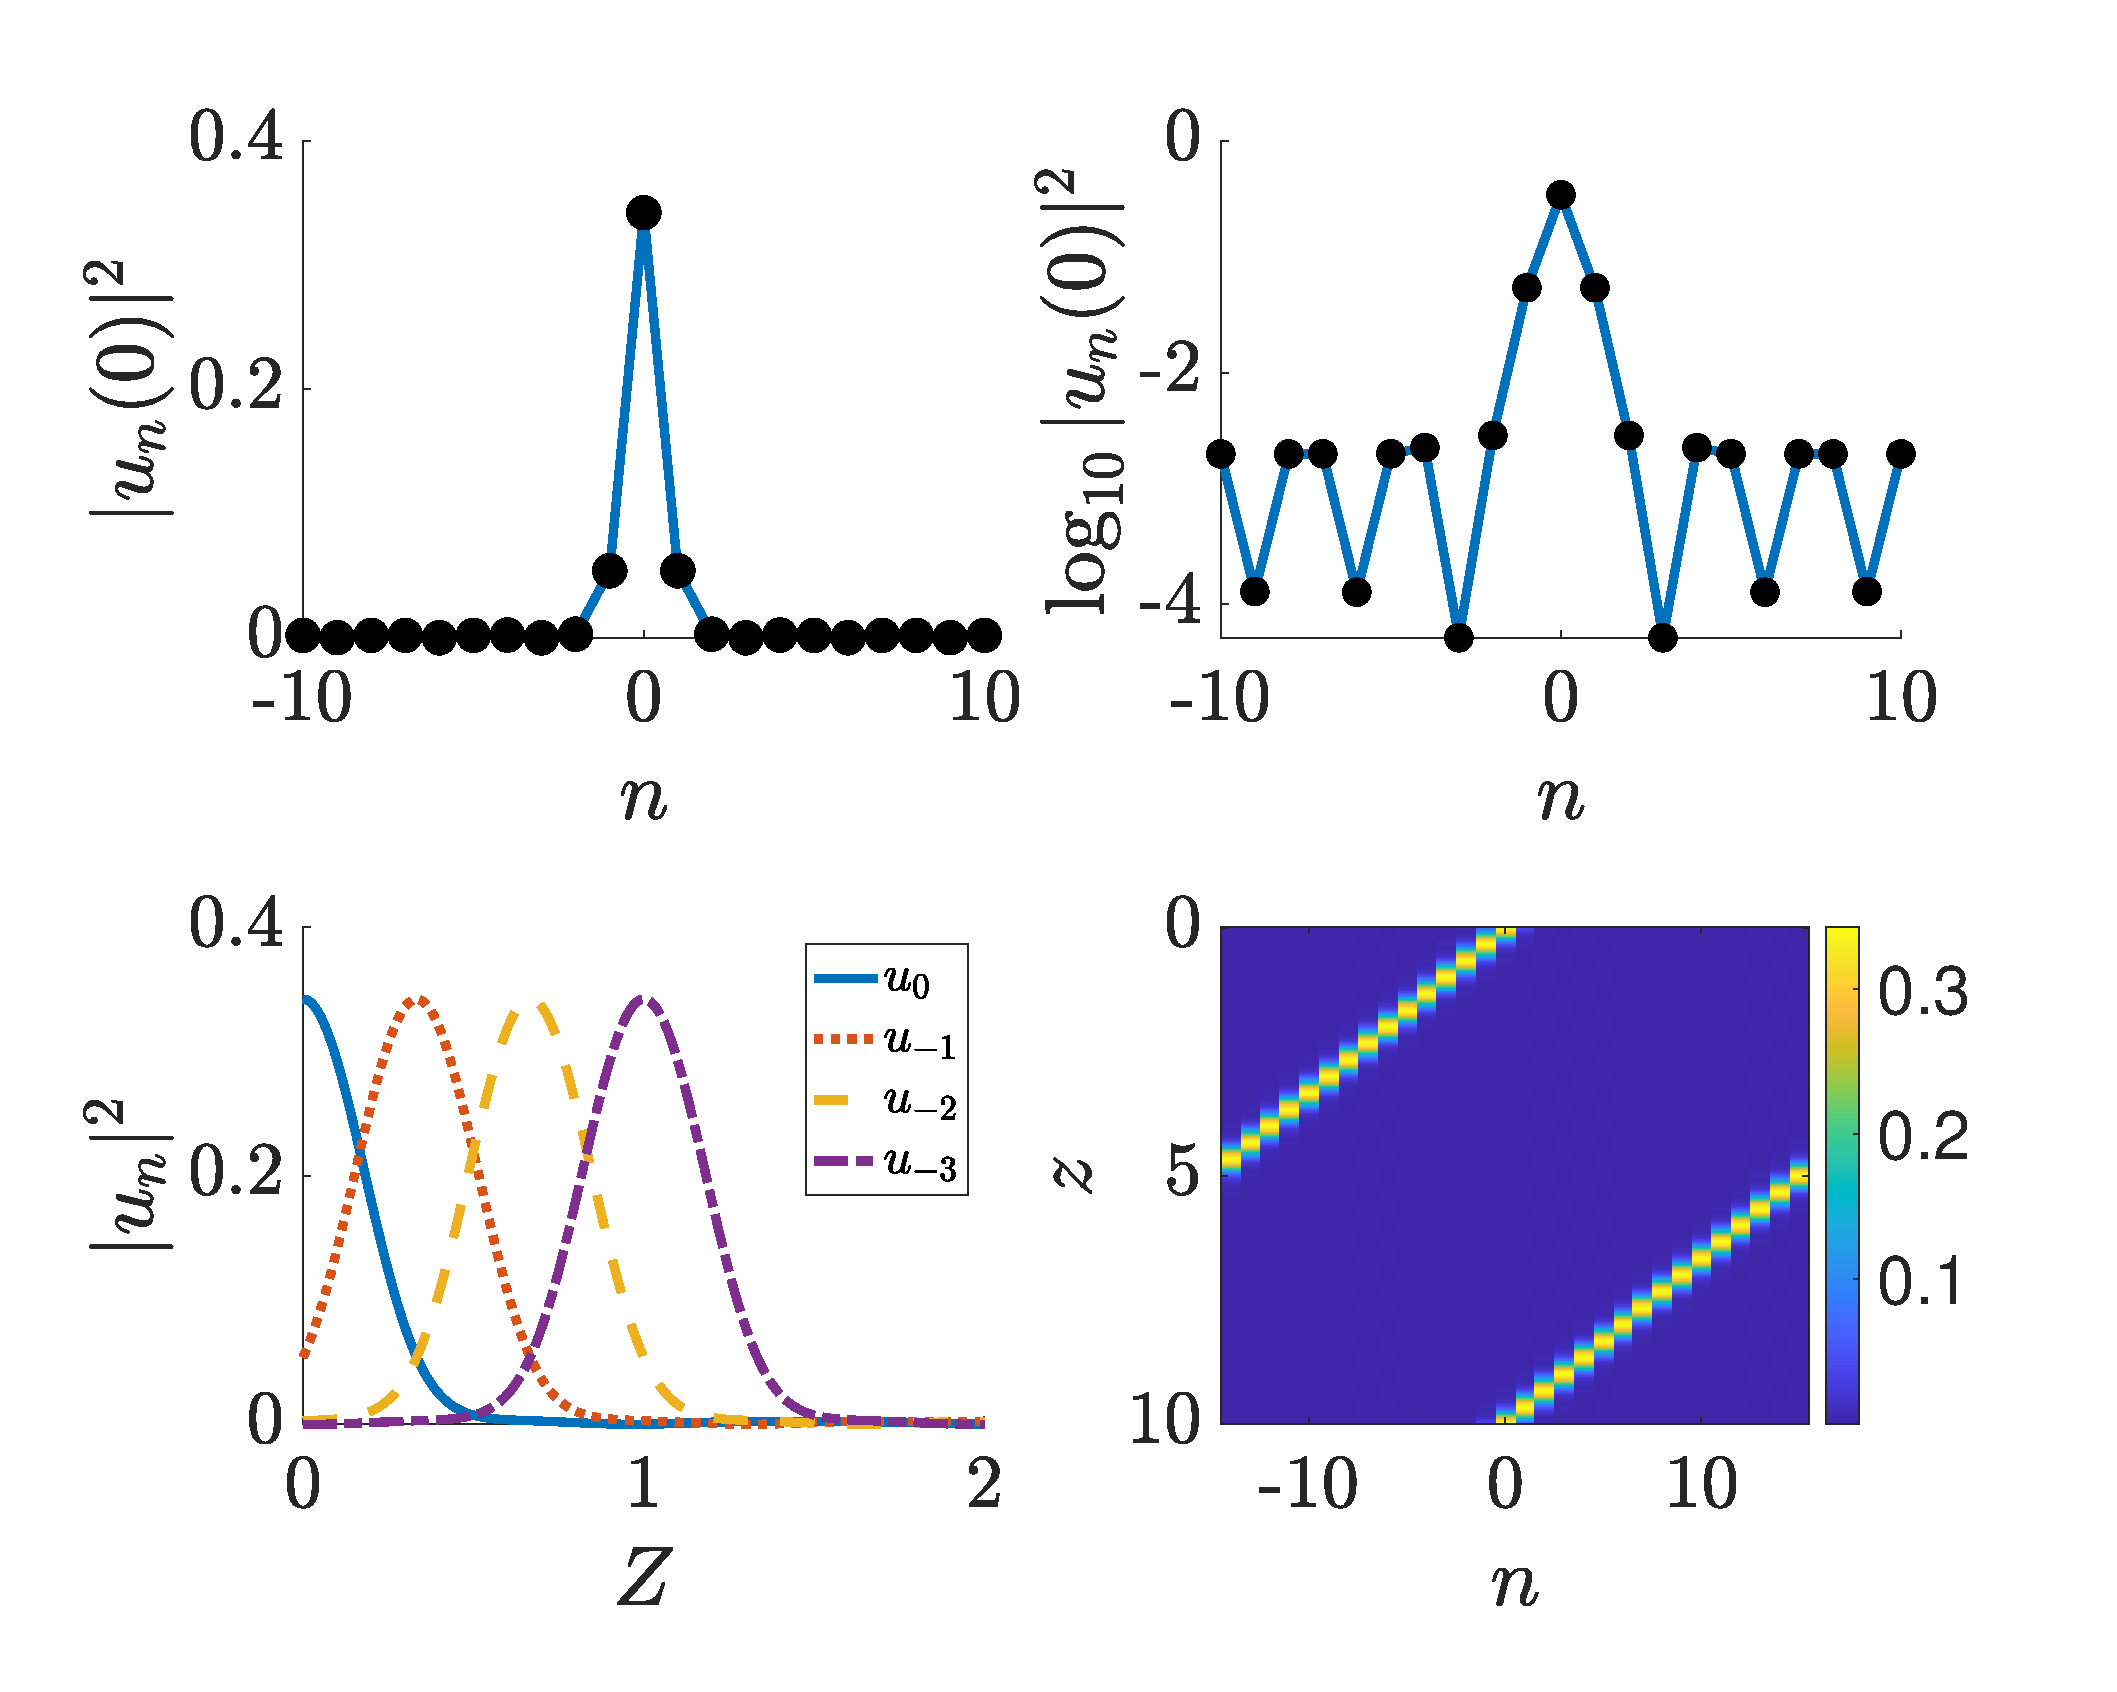
\includegraphics[width=9cm]{leftsol.eps}
    \caption{Initial intensity $|u_n(0)|^2$ (top left) and log of initial intensity (top right) for left-moving solution. The intensity of the solution evolved in $Z$ over a period is presented for a few select sites (bottom left), and the space-time contour 
    plot evolution of the intensity for the traveling wave is also shown (bottom right).}
    \label{fig:leftsol}
\end{figure}

\begin{figure}
    \centering
    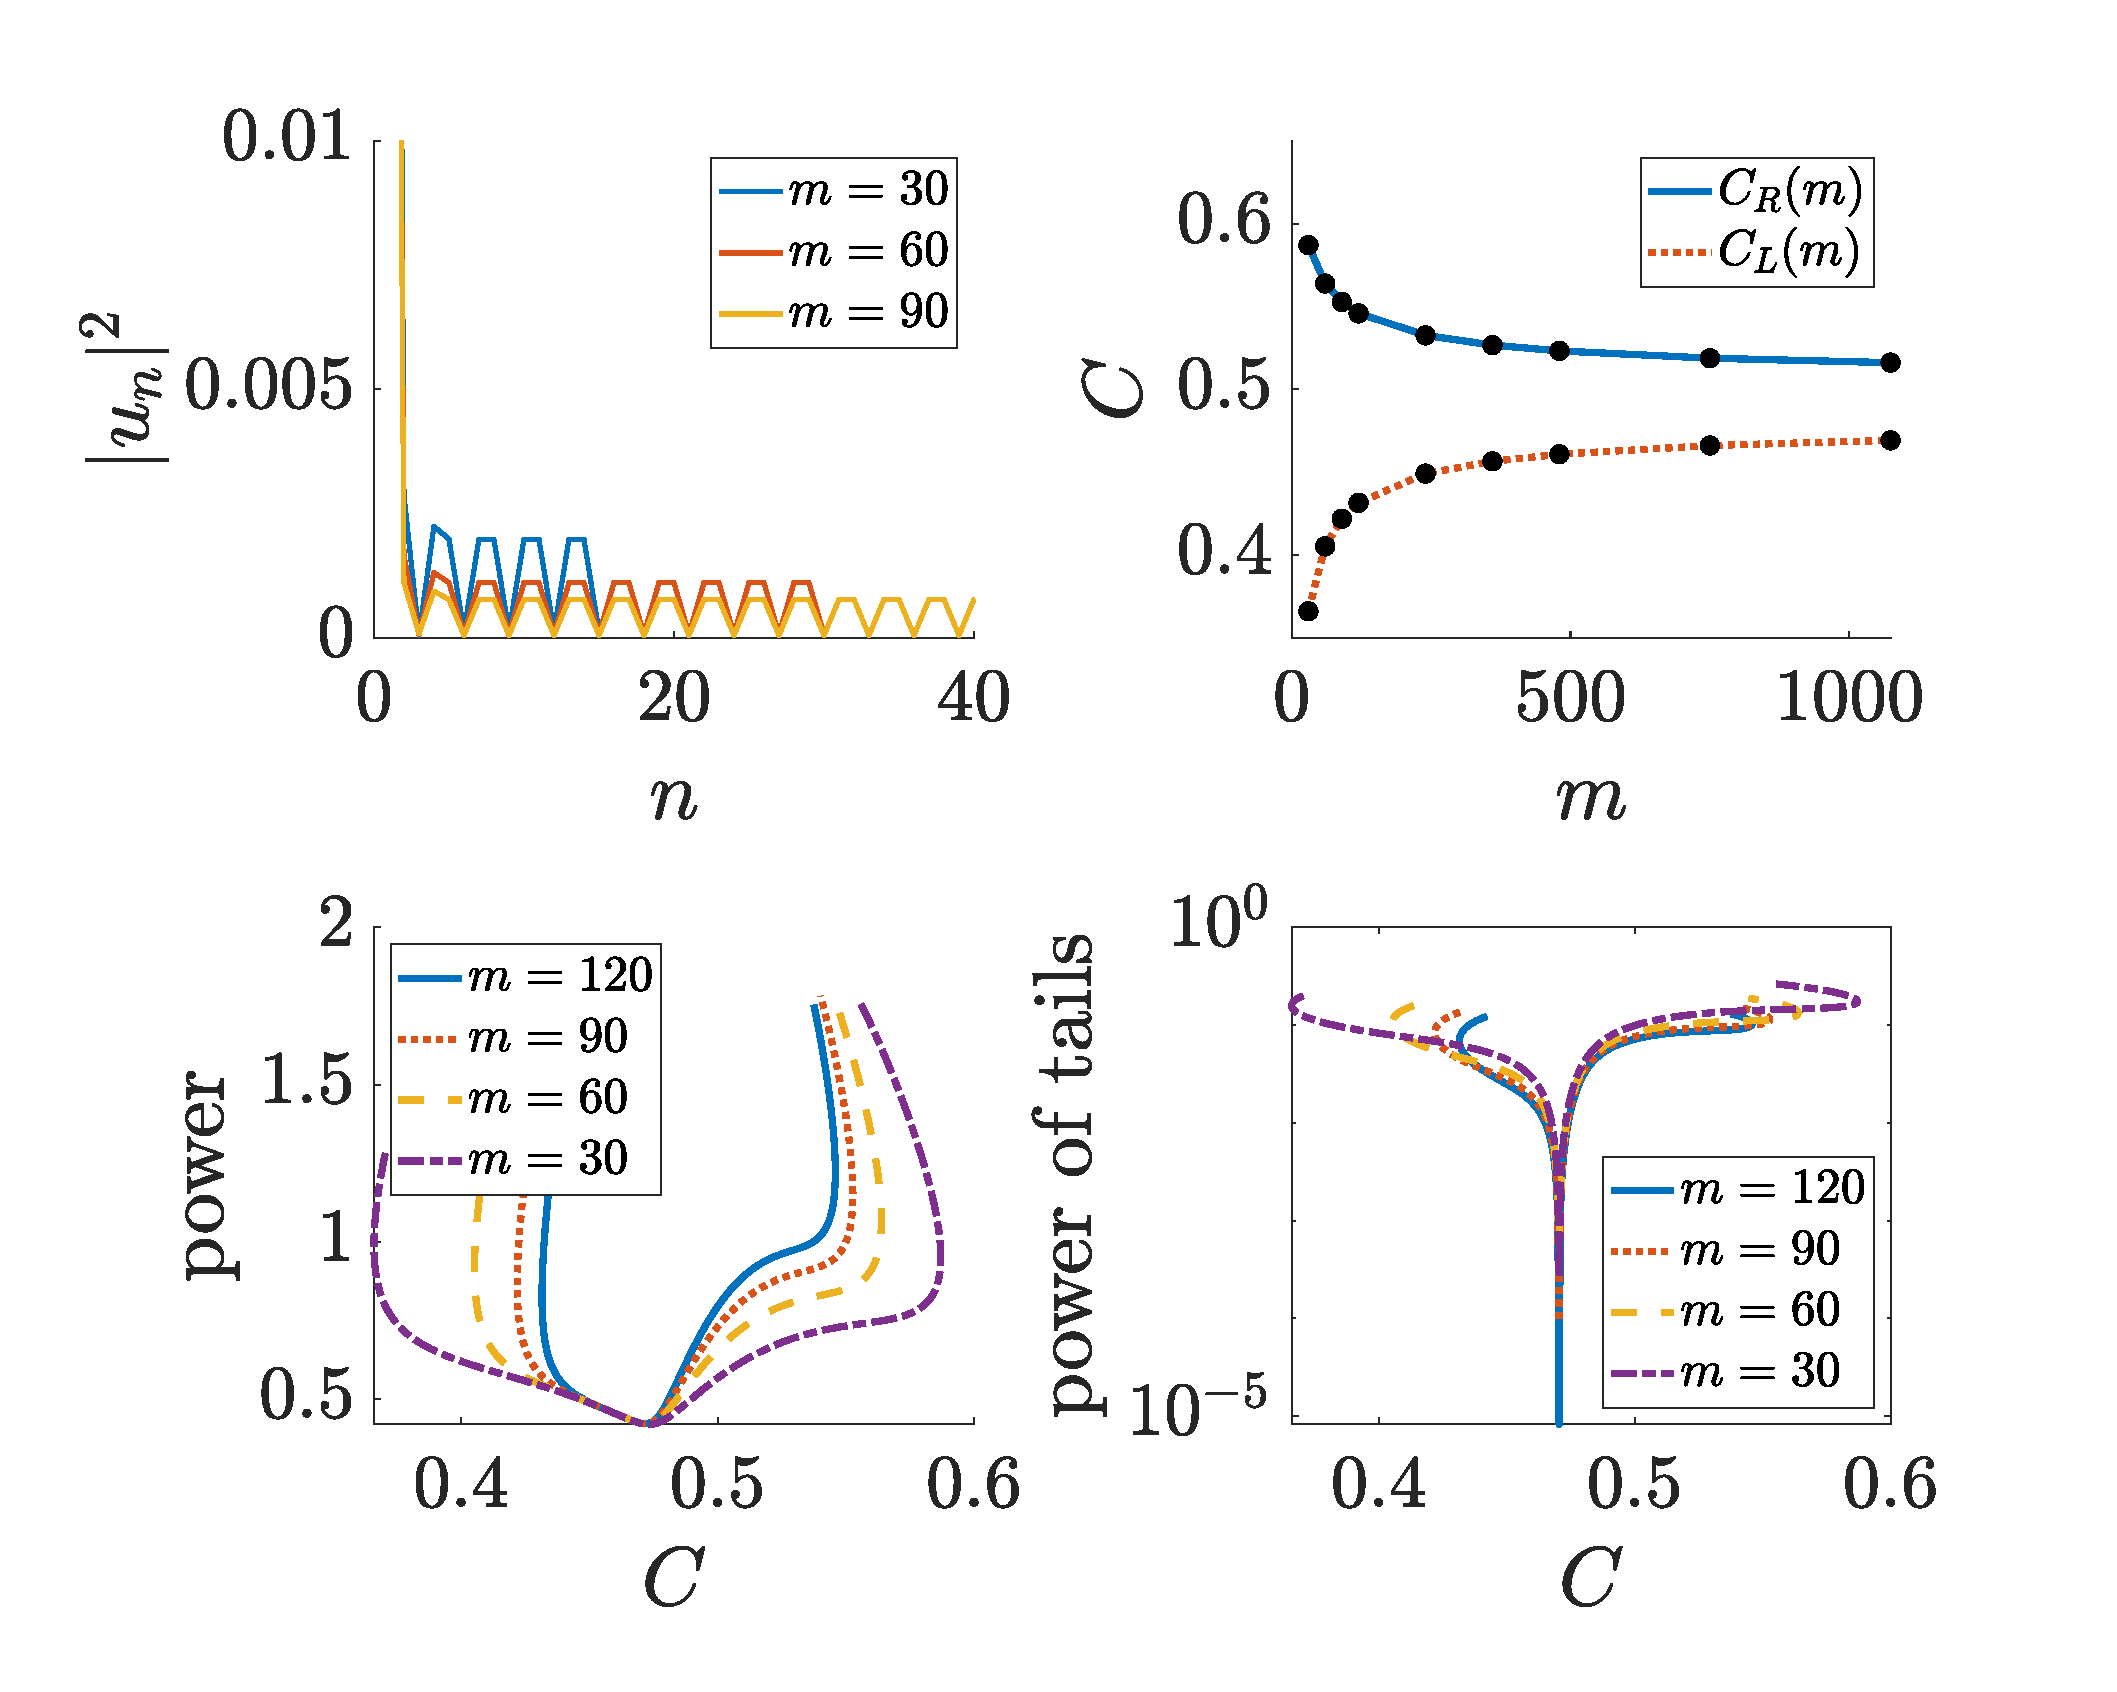
\includegraphics[width=9cm]{leftdiag.eps}
    \caption{Top left: plot of intensity of the tails for the left-moving solution and for 3 values of the lattice size $m$. Top right: interval of existence $[C_L(m),C_R(m)]$ of left-moving solution. Bottom left: power of left-moving solution vs. $C$ for parameter
    % Comment: did you indeed mean the total power here??
    continuation in $C$. Bottom right: maximum intensity of the tails for the left-moving solution vs. $C$. Minimum is at $C^* = 0.4709$ for all lattice sizes $m$.}
    \label{fig:leftdiag}
\end{figure}

\begin{figure}
    \centering
    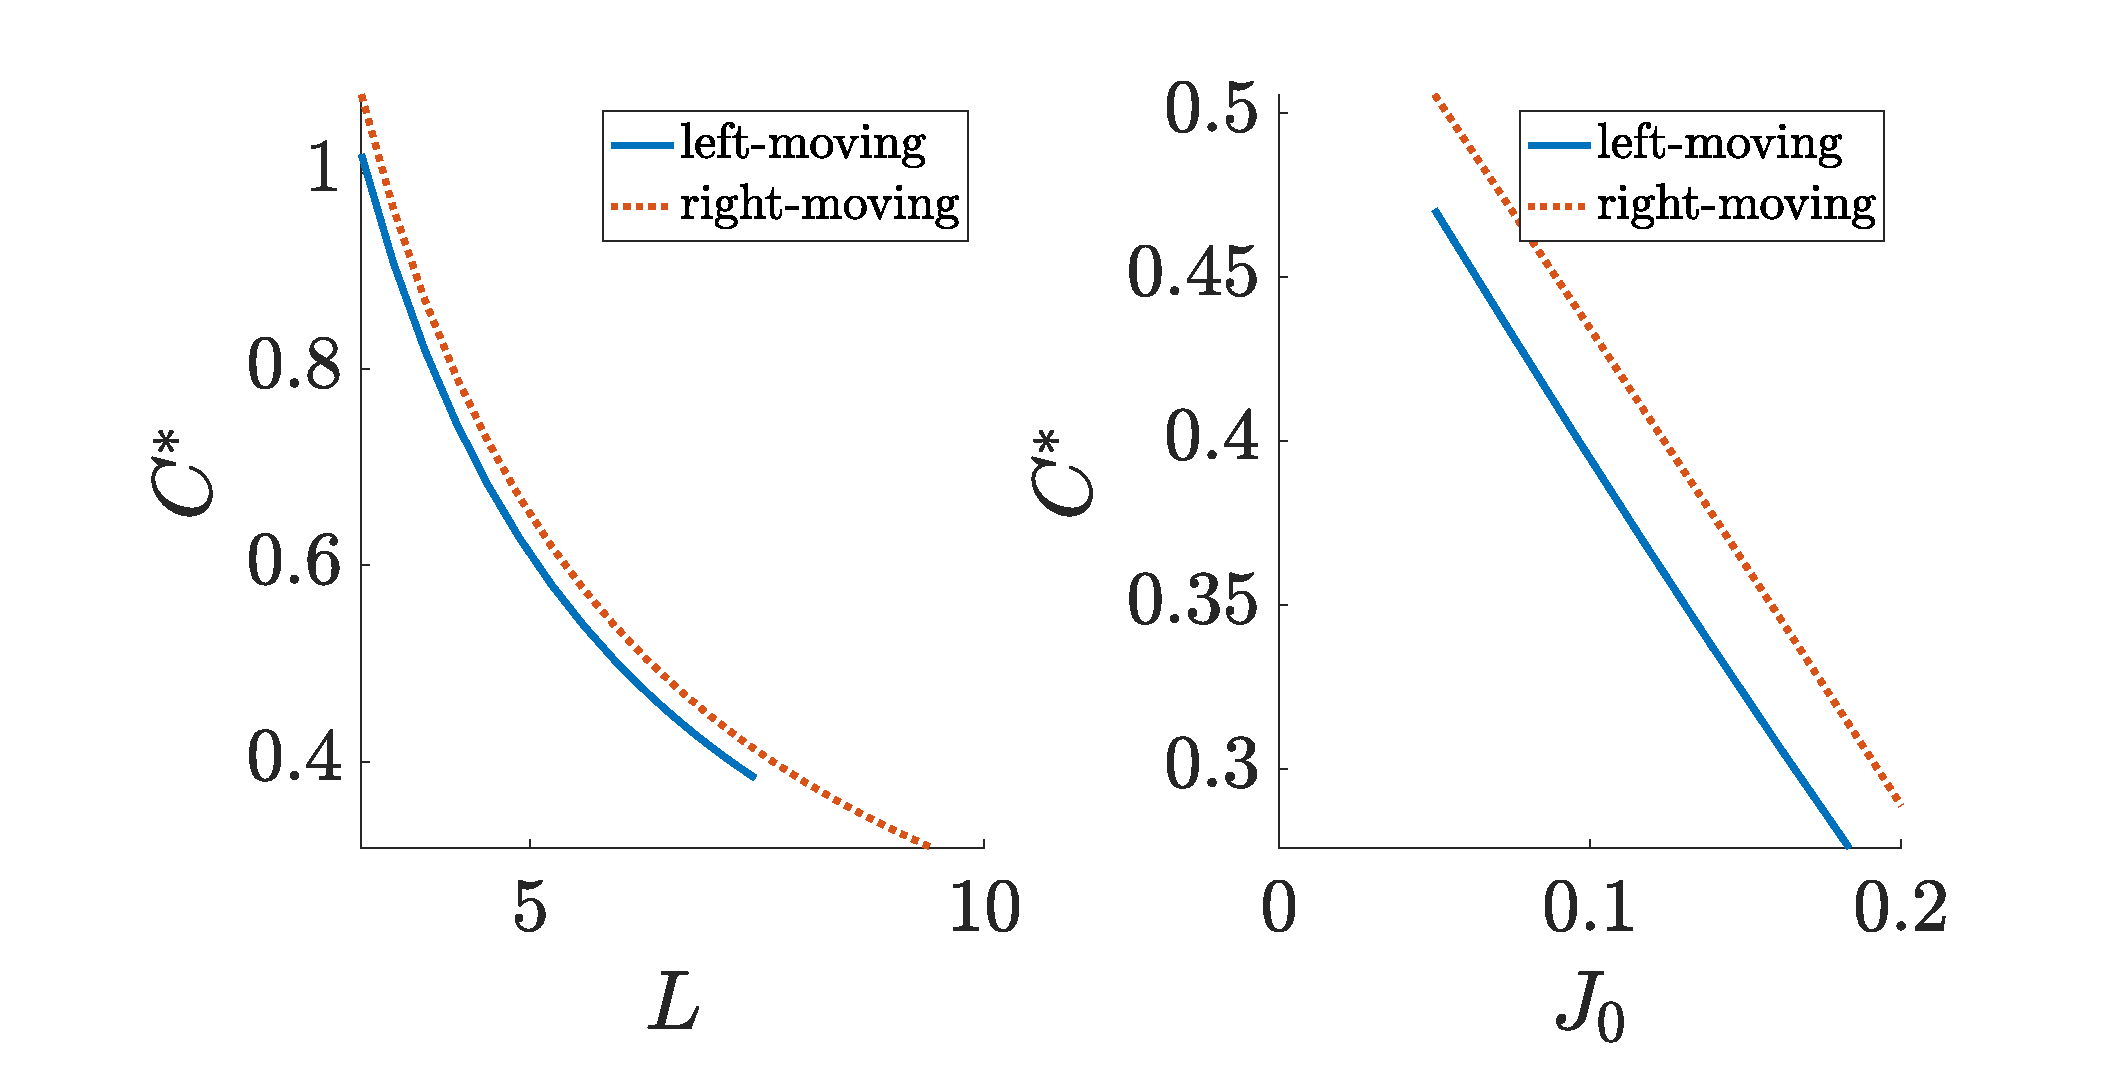
\includegraphics[width=9cm]{Cstar.eps}
    \caption{Plot of critical value $C^*$ of $C$ at which the intensity of the 
    tails of left- and right-moving solutions is a minimum vs. $L$ (left) and $J_0$ (right).} % JCM: what are the values of J_0 and C in the left and right panels, respectively?
    \label{fig:Cstar}
\end{figure}

\begin{figure}
    \centering
    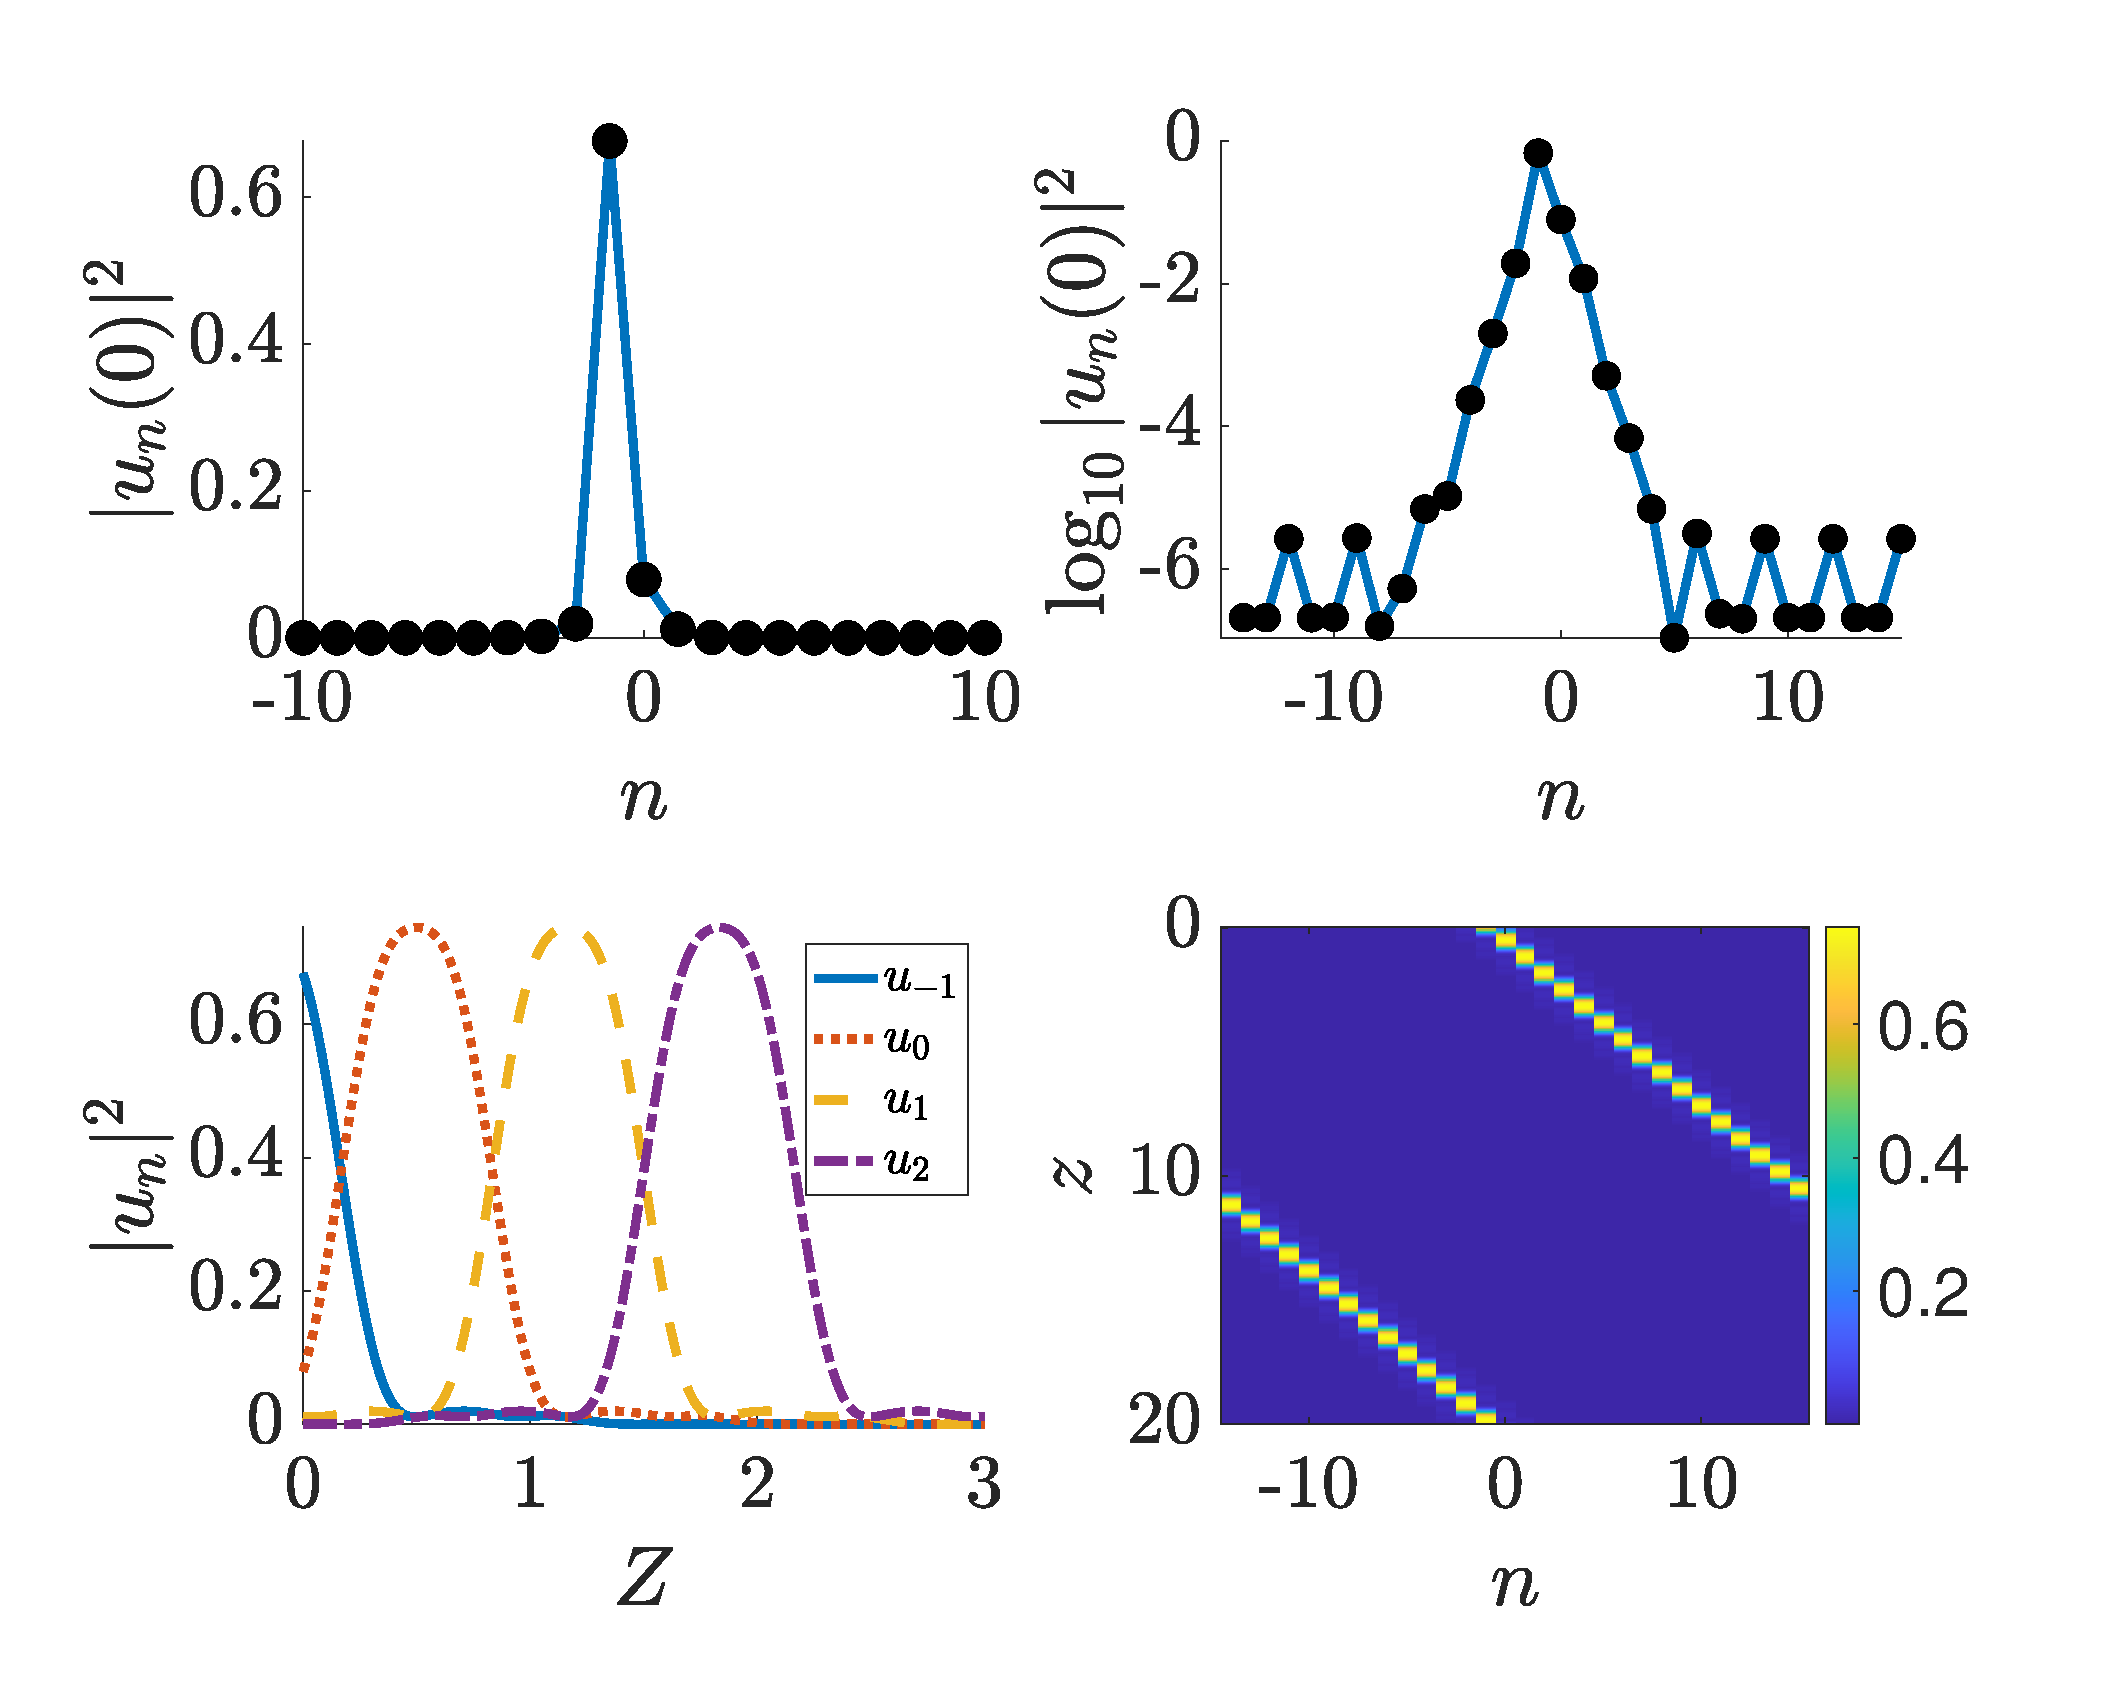
\includegraphics[width=9cm]{rightsol.eps}
    \caption{Initial intensity $|u_n(0)|^2$ (top left) and log of initial intensity (top right) for right moving solution. The intensity of the solution evolved in $Z$ over a period is presented for a few select sites (bottom left), and the space-time contour 
    plot evolution of the intensity for the traveling wave is also shown (bottom right).}
    \label{fig:rightsol}
\end{figure}

\begin{figure}
    \centering
    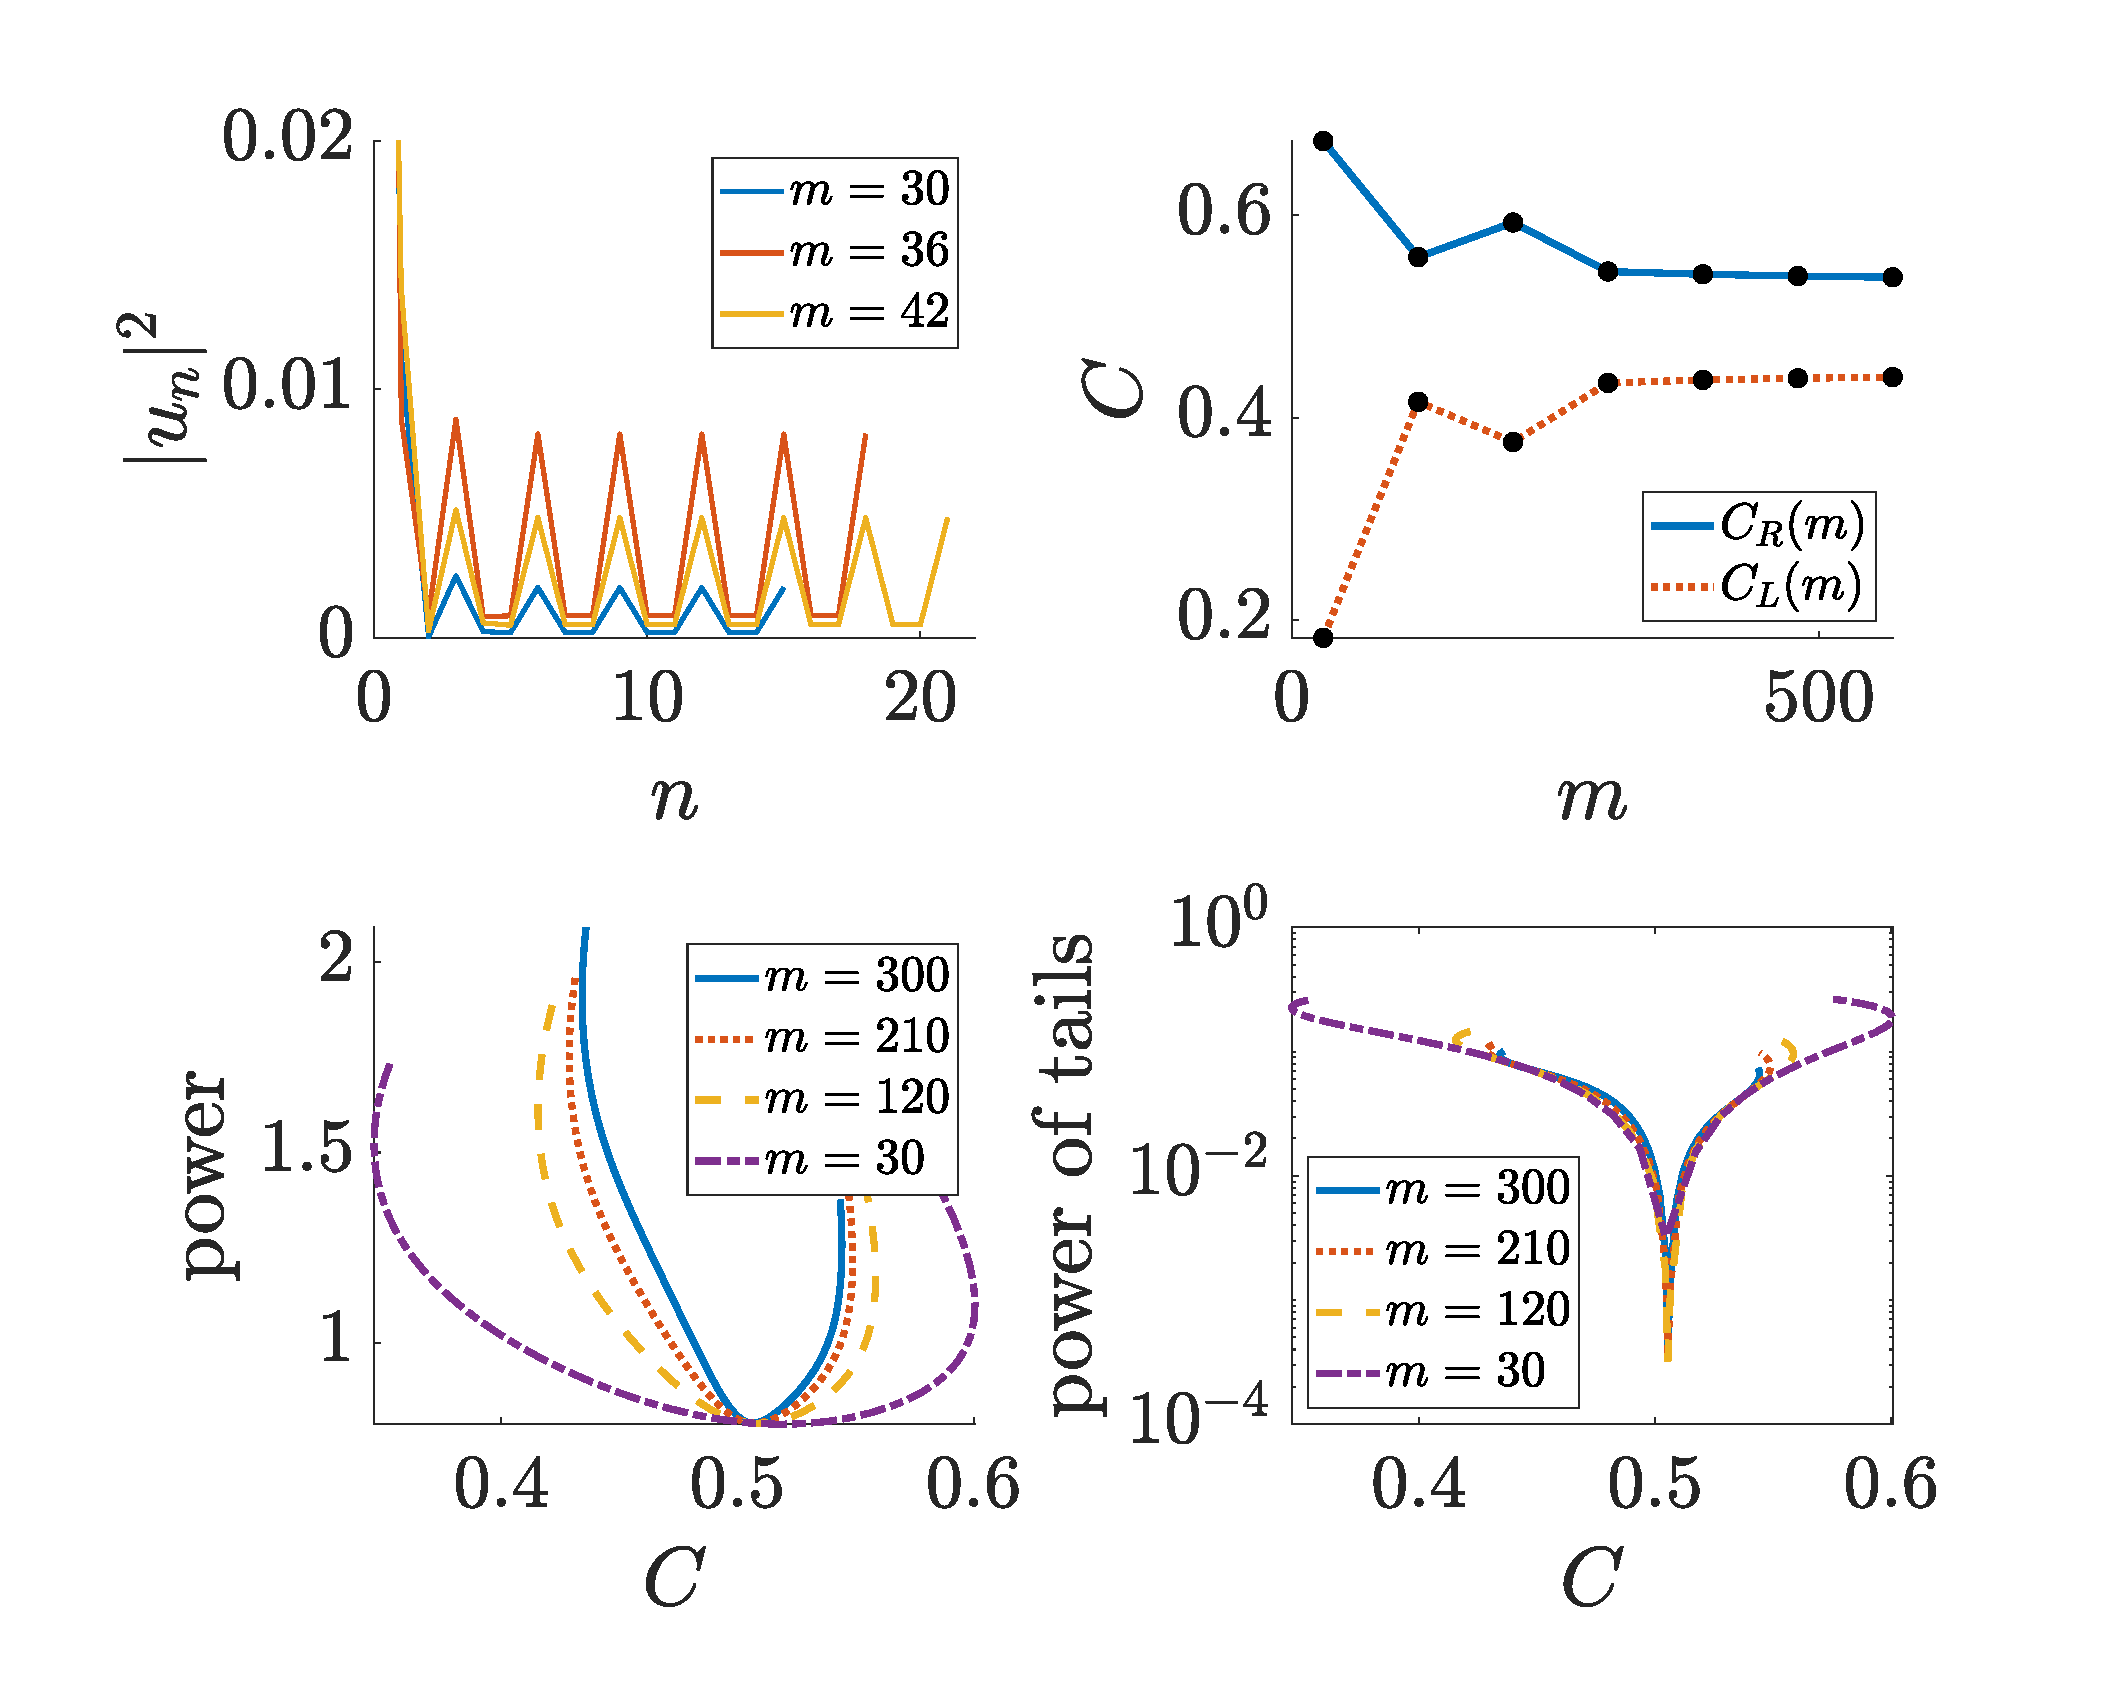
\includegraphics[width=9cm]{rightdiag.eps}
    \caption{Top left: plot of power of of tails of of right-moving solution for 3 values of the lattice size $m$. Top right: interval of existence $[C_L(m),C_R(m)]$ of right-moving solution. Bottom left: power of right-moving solution vs. $C$ for parameter continuation in $C$. Bottom right: maximum power of tails of right-moving solution vs. $C$. Minimum is at $C^* = 0.5054$ for all lattice sizes $m$.}
    \label{fig:rightdiag}
\end{figure}

\begin{figure}
    \centering
    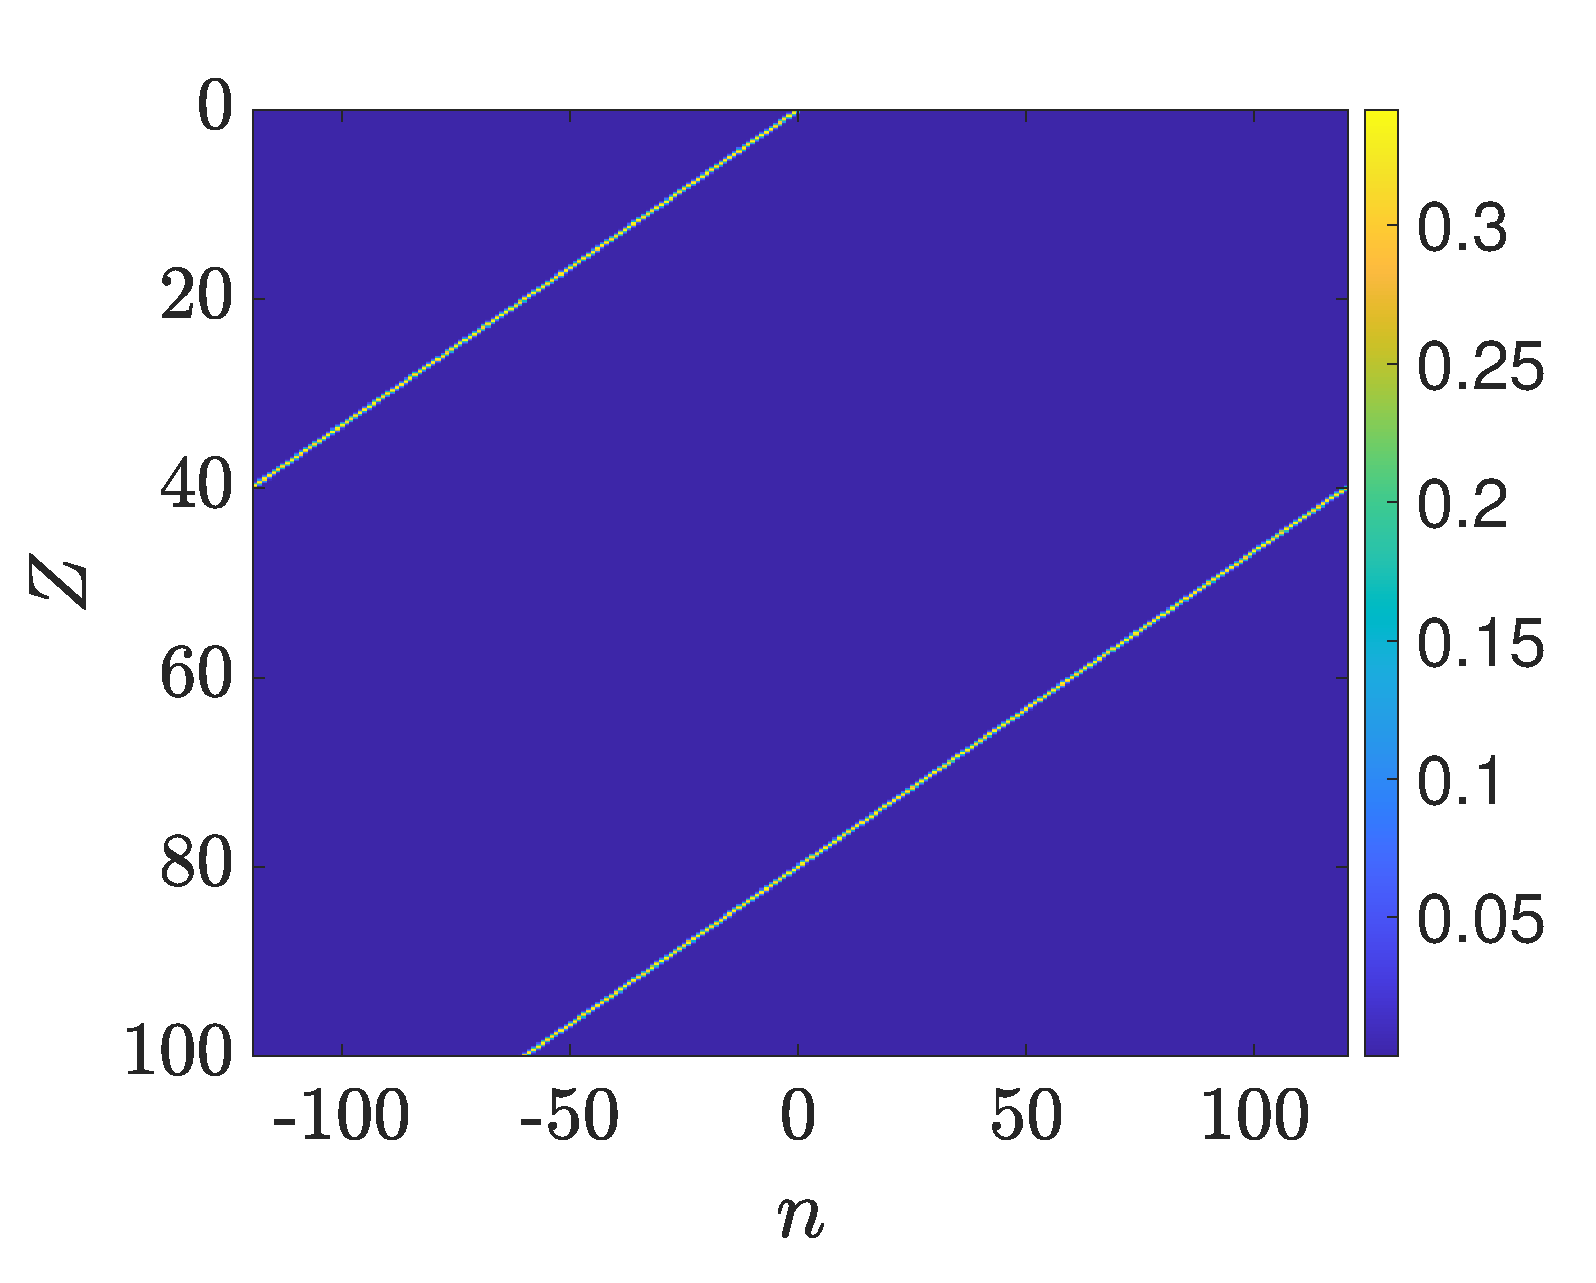
\includegraphics[width=3.90cm]{leftlong.eps}
    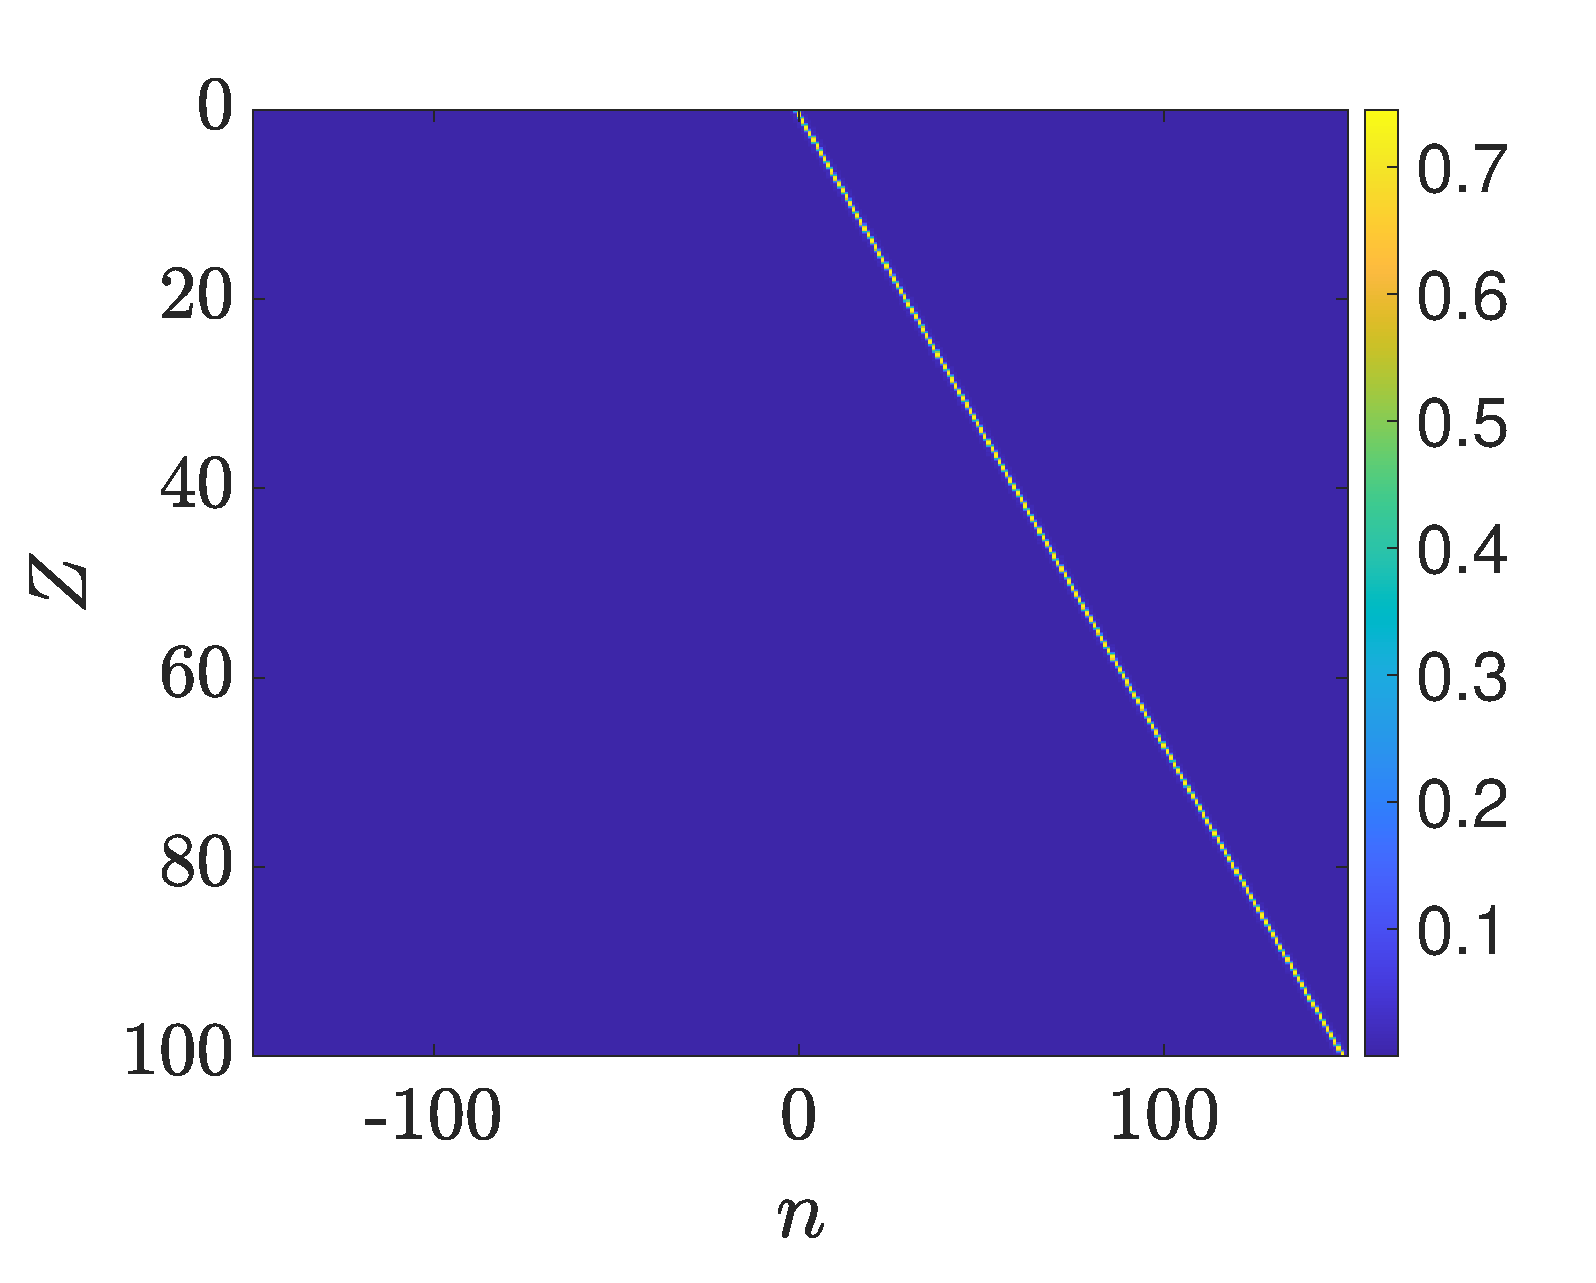
\includegraphics[width=3.90cm]{rightlong.eps}
    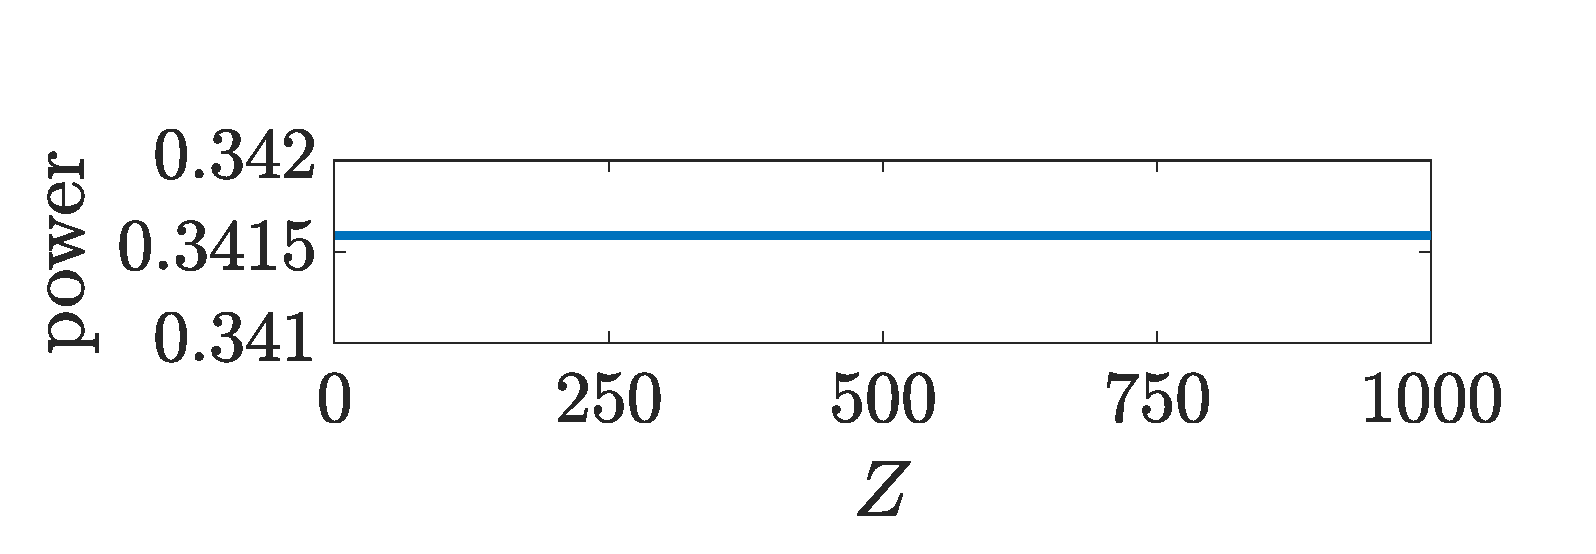
\includegraphics[width=3.90cm]{leftperiods.eps}
    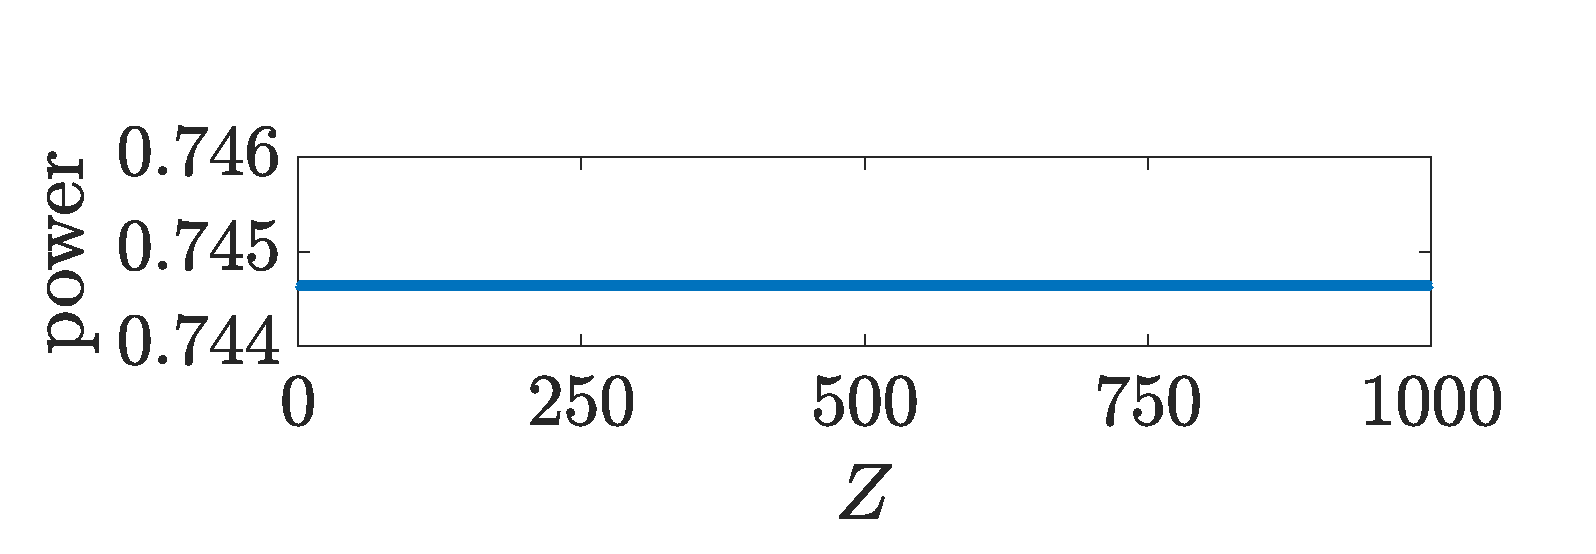
\includegraphics[width=3.90cm]{rightperiods.eps}
    \caption{Top: colormap of long term evolution in $Z$ of left-moving solution (left, $C=0.4703$, $m=240$) and right-moving solution (right, $C=0.5054$, $m=300$) for $C=C^*$. Bottom: power of site with peak intensity of moving solution over 1000 periods.}
    \label{fig:movelong}
\end{figure}

% JCM: I think we should make a comment on the relationship between the right- and left-moving solutions and the Chern number

\subsection{Collisions}\label{sec:collisions}

Finally, we briefly explore the resulting phenomenology when a left-moving and a right-moving solution collide, an event shown in \cref{fig:collision1}. For the
relevant initial condition, we splice together well-separated copies of the left-moving and right-moving solutions. To avoid combining the tail oscillations of the two solutions, we choose to simulate such a scenario when $C=C^*$ for the left-moving solution, so that its tail oscillations are suppressed. 
In a different case, the tail oscillations would superpose producing
more drastic events of dispersive radiation wavepackets throughout the course
of our simulations.
We see that both solutions emerge from the first collision, but both solutions lose power as intensity radiates to the left. Power is lost with each subsequent collision (\cref{fig:collision1}, bottom) within the periodic ring of our domain. Accordingly,
the waveforms keep disintegrating (a feature possible due to the non-integrability
of the solitary waves) as a progressive outcome of the relevant collisions.

\begin{figure}
    \centering
    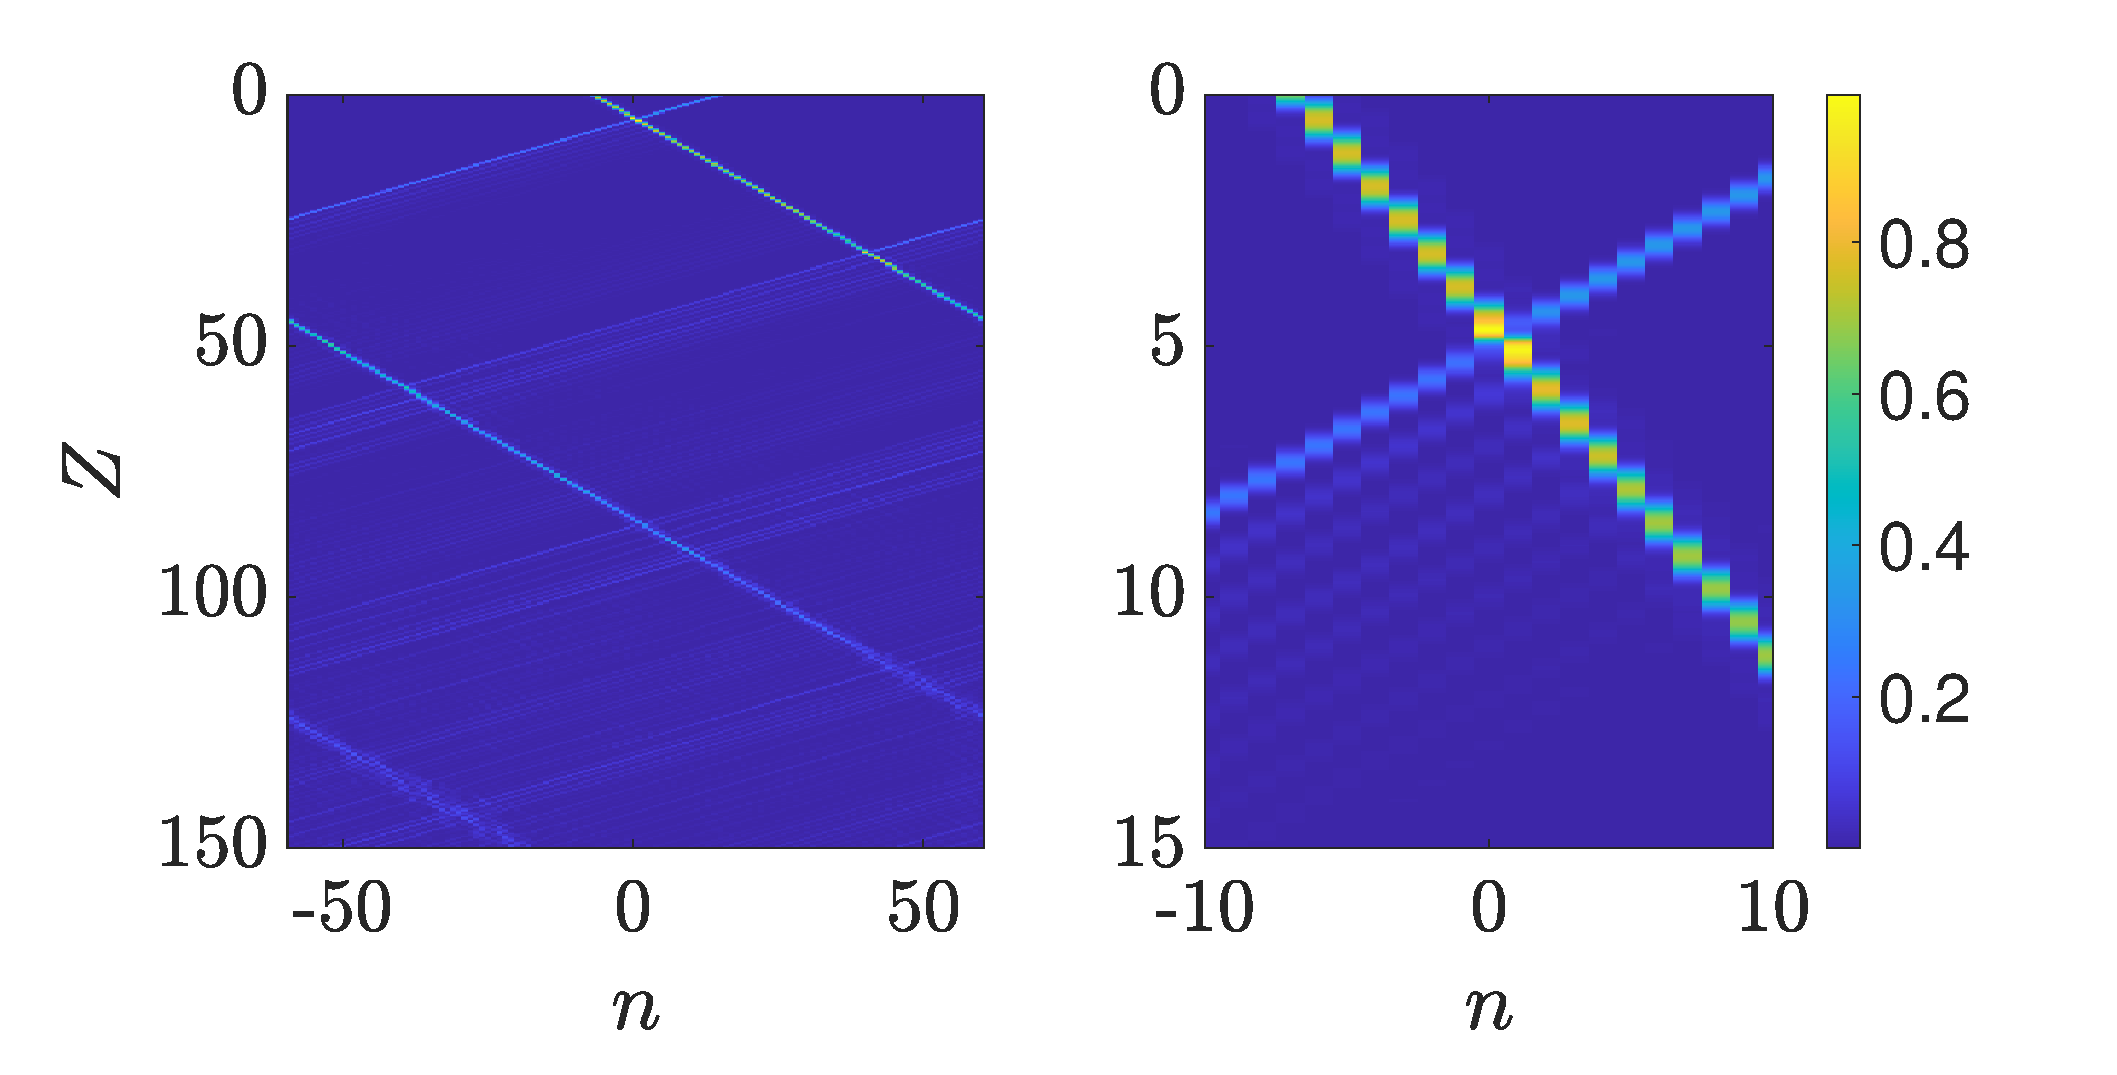
\includegraphics[width=9cm]{images/collision1.eps}
    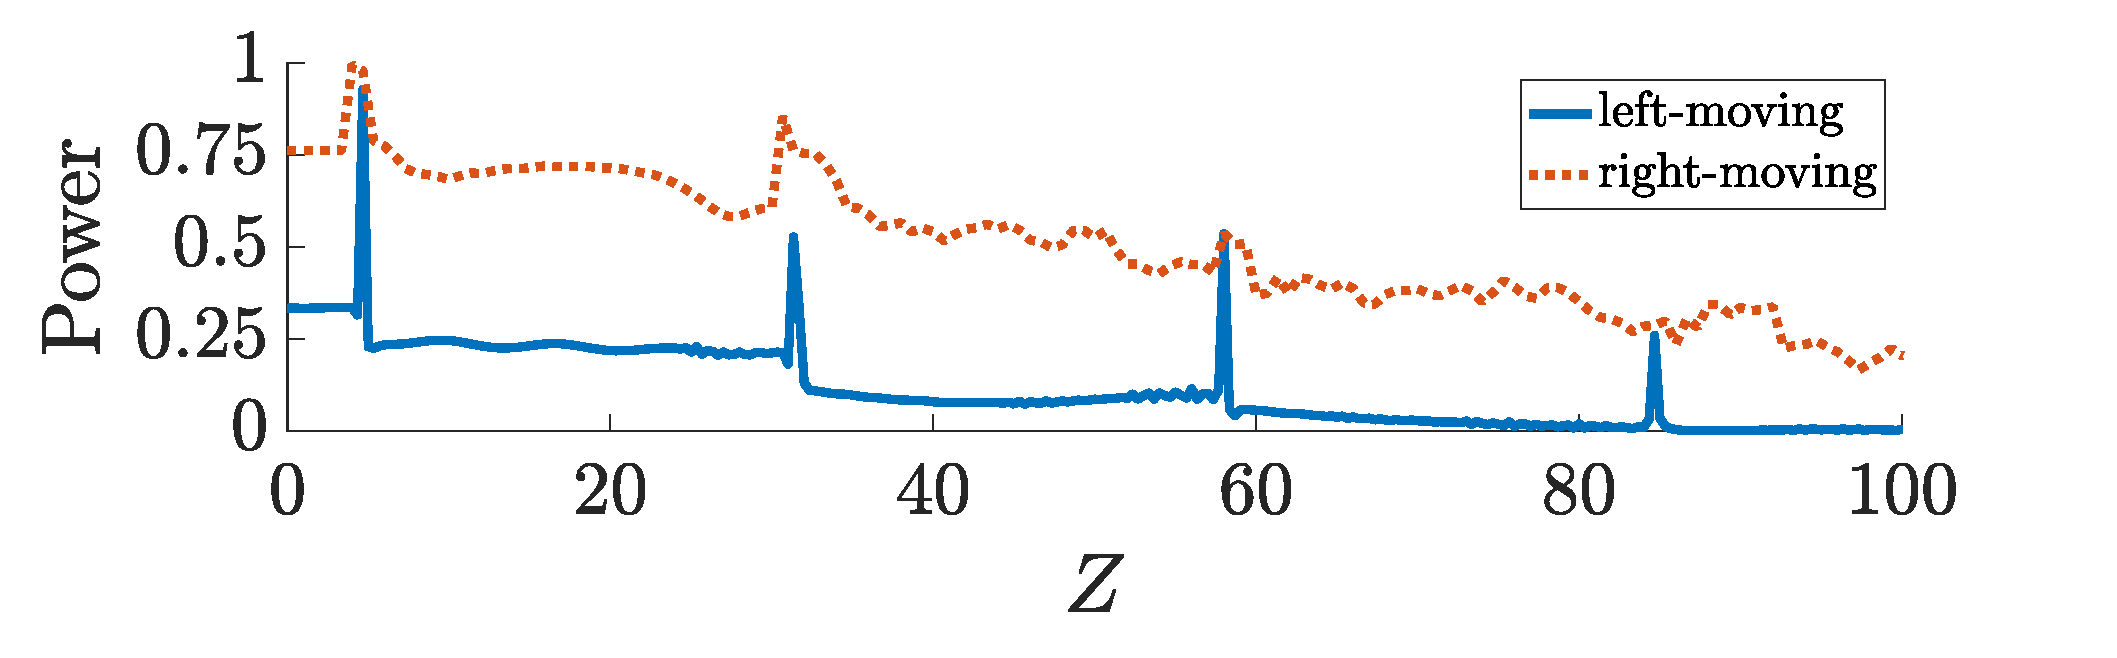
\includegraphics[width=9cm]{images/collision1power.eps}
    \caption{Top: Colormap of evolution in $Z$ and space denoted by $n$ of the collision between left-moving and right-moving solution. The right panel is a zoomed-in view of the first collision, representing more clearly the power loss that the waves incur as
    a result. Bottom: evolution  of the site with peak intensity for the profile bearing the left- and right-moving solutions.
    $m=120$, $C=0.4703$.}
    \label{fig:collision1}
\end{figure}

\section{Conclusions and Future Directions}\label{sec:conclusions}

In the present work, we have studied coherent structures in a one-dimensional 
optical waveguide array with periodically modulated coupling function, directly
motivated by a sequence of impactful physical experiments in the work of~\cite{Mukherjee2020,recht21,PhysRevLett.128.113901,Jurgensen2021}. We have found that the system exhibits two fundamental coherent structures in which the bulk of the intensity is concentrated on a single site. At low intensity, we find moving solutions, in which the intensity propagates leftward or rightward in the lattice. The direction and speed of propagation depend on which site is initially excited; this can be explained in terms of the coupling function which is most active at a given $z$. At high intensity, we find stationary solutions, which are periodic orbits of the system. By analyzing a simplification of the model where the couplings between waveguides are given by step functions, we are able to explain this behavior by looking at an effective dimer setting, which features
the celebrated self-trapping transition.  Indeed, in the dimer, when the couplings do not change,  there is a sharp transition between solutions in which power is completely transferred back and forth between the two adjacent nodes and ones in which the power is mainly confined to one of the fibers. For larger lattices, the couplings change three times every spatial period. This ``interrupts'' the power transfer in the dimer, which explains the fact that the sharp transition is now ``smoothened'' (i.e., is more gradual) in larger lattices. 
Nevertheless, the principal phenomenology is still present, as is also revealed by the
direct comparison of the two models (the original one and the variant with the step functions).
Using Floquet analysis, we find that the stationary coherent structures are stable for a wide range of parameters. The moving solutions are characterized by small-amplitude, oscillatory tails, whose amplitude and configuration depends on the lattice size. There is, however, a critical set of parameters for which these tail oscillations disappear. Interestingly, these critical parameters do not depend on the lattice size, and the moving solution appears to be stable for these parameters.

One potential avenue for future investigation would be examine what happens for very large spatial period $L$, which is the regime studied in \cite{Jurgensen2021}. Using our numerical parameter continuation methods, this would require starting with very large power single-site solutions at $C=0$ (see \cref{fig:statcontL}). So far, this has not been found to be computationally feasible, and would likely require a different numerical approach
(indeed, an adiabaticity-based one was used earlier in~\cite{Jurgensen2021}). Another direction would be to explore the solutions on the upper branches of the bifurcation diagram in \cref{fig:statAC}. These solutions, to leading order, involve Fourier modes of two different wavenumbers. To the best of our knowledge, these have never been investigated. Finally, although we expect that the qualitative behavior will be the same for similar coupling functions, we could explore similar systems with unit cells comprising different numbers of sites. For a two-site unit cell, there would be left-right symmetry, and we expect that the rightward- and leftward-moving solutions would be mirror images of each other. It would be interesting to investigate what occurs if the unit cell comprises more than three sites, a setting that has also been explored in the above experiments.
Furthermore, in the vein of the earlier work of~\cite{PhysRevE.105.044211}, understanding
the impact of higher-dimensions (and possibly topological lattices therein) in the relevant
phenomenology would also be of substantial interest.

\begin{acknowledgments}
This material is based upon work supported by the U.S. National Science Foundation under the RTG grant DMS-1840260 (R.P. and A.A.), PHY-2110030 (P.G.K.), and DMS-1909559 (A.A.). J.C.-M. acknowledges support from EU (FEDER program 2014-2020) through both Consejería de Economía, Conocimiento, Empresas y Universidad de la Junta de Andalucía (under the projects P18-RT-3480 and US-1380977), and MICINN and AEI (under the projects PID2019-110430GB-C21 and PID2020-112620GB-I00).
\end{acknowledgments}

\bibliographystyle{apsrev4-2}
\bibliography{main.bib}

\end{document}